%%%%%%%%%%%%%%%%%%%%%%%%%%%%%%%%%%%%%%%%%%%%%%%
%
% Template per Elaborato di Laurea
% DISI - Dipartimento di Ingegneria e Scienza dell’Informazione
%
% update 2015-09-10
%
% Per la generazione corretta del
% pdflatex nome_file.tex
% bibtex nome_file.aux
% pdflatex nome_file.tex
% pdflatex nome_file.tex
%
%%%%%%%%%%%%%%%%%%%%%%%%%%%%%%%%%%%%%%%%%%%%%%%

% formato FRONTE RETRO
\documentclass[epsfig,a4paper,11pt,titlepage,oneside,openany]{book}
\usepackage{epsfig}
\usepackage{plain}
\usepackage{setspace}
\usepackage[paperheight=29.7cm,paperwidth=21cm,outer=1.5cm,inner=2.5cm,top=2cm,bottom=2cm]{geometry} % per definizione layout
\usepackage{titlesec} % per formato custom dei titoli dei capitoli
\usepackage{multicol}
\usepackage{float}
\usepackage{svg}
\usepackage{subfig}
\usepackage{makecell}
\renewcommand*{\thesubfigure}{(\arabic{subfigure})}
%%%%%%%%%%%%%%
% supporto lettere accentate
%
%\usepackage[latin1]{inputenc} % per Windows;
\usepackage[utf8x]{inputenc} % per Linux (richiede il pacchetto unicode);
%\usepackage[applemac]{inputenc} % per Mac.

\singlespacing

\usepackage[italian]{babel}

\begin{document}

  % nessuna numerazione
  \pagenumbering{gobble}
  \begin{titlepage}
\pagestyle{plain}

\thispagestyle{empty}

\begin{center}
  \begin{figure}[h!]
    \centerline{
\psfig{file=prefixes/images/marchio_unitrento_colore_it_202002.eps,width=0.6\textwidth}}
  \end{figure}

  \vspace{2 cm} 

  \LARGE{Dipartimento di Ingegneria e Scienza dell’Informazione\\}

  \vspace{1 cm} 
  \Large{Corso di Laurea in\\
    Informatica
    %Ingegneria dell'Informazione e delle Comunicazioni
    %Ingegneria dell'Informazione e Organizzazione d'Impresa
    %Ingegneria Elettronica e delle Telecomunicazioni
  }

  \vspace{2 cm} 
  \Large\textsc{Elaborato finale\\} 
  \vspace{1 cm} 
  \Huge\textsc{Analysis of RNA-seq transcriptomic data from total and polysomal mRNA fractions from an epithelial cancer cell line\\}


  \vspace{2 cm} 
  \begin{tabular*}{\textwidth}{ c @{\extracolsep{\fill}} c }
  \Large{Supervisore} & \Large{Laureando}\\
  \Large{......}& \Large{Giacomo Fantoni}\\
  \end{tabular*}

  \vspace{2 cm} 

  \Large{Anno accademico 2020/2021}
  
\end{center}
\end{titlepage}


  \clearpage
%%%%%%%%%%%%%%%%%%%%%%%%%%%%%%%%%%%%%%%%%%%%%%%%%%%%%%%%%%%%%%%%%%%%%%%%%%
%%%%%%%%%%%%%%%%%%%%%%%%%%%%%%%%%%%%%%%%%%%%%%%%%%%%%%%%%%%%%%%%%%%%%%%%%%
%% Nota
%%%%%%%%%%%%%%%%%%%%%%%%%%%%%%%%%%%%%%%%%%%%%%%%%%%%%%%%%%%%%%%%%%%%%%%%%%
%% Sezione Ringraziamenti opzionale
%%%%%%%%%%%%%%%%%%%%%%%%%%%%%%%%%%%%%%%%%%%%%%%%%%%%%%%%%%%%%%%%%%%%%%%%%%
%%%%%%%%%%%%%%%%%%%%%%%%%%%%%%%%%%%%%%%%%%%%%%%%%%%%%%%%%%%%%%%%%%%%%%%%%%
  \thispagestyle{empty}

\begin{center}
  {\bf \Huge Ringraziamenti}
\end{center}

\vspace{4cm}
\emph{Vorrei ringraziare i miei genitori Elisabetta e Corrado per avermi permesso di intraprendere questo percorso e per avermi aiutato a diventare la persona che vorrei essere.\\[12pt]
	Ringrazio mio zio Enrico per avermi accompagnato in Universit\`a questi tre anni.\\[12pt]
	Ringrazio inoltre i miei relatori per avermi seguito cos\`i attentamente durante lo svolgimento di questo lavoro e per avermi dato gli strumenti necessari a compiere questo lavoro.\\[12pt]
	Ringrazio il mio professore di informatica delle superiori Marco per avermi fatto scoprire le gioie del mondo informatico.\\[12pt]
	Ringrazio la mia collega Elisa per avermi accompagnato durante la produzione di questo progetto e per il sostegno che ci siamo dati durante questo percorso.\\[12pt]
	Ringrazio Daniele per avermi sempre supportato e per aver sempre sopportato i miei infiniti discorsi su questo argomento.\\[12pt]
	Ringrazio le mie coinquiline, Sofia e Cecilia, per la compagnia e l'amicizia nata in questi tre anni di universit\`a e per aver reso la mia prima esperienza di vita da solo cos\`i piacevole.\\[12pt]
	Ringrazio infine la mia fidanzata Giovanna, per quest'ultimo anno fantastico e per avermi dato il coraggio di proseguire sempre con serenit\`a.
}

  \clearpage
  \pagestyle{plain} % nessuna intestazione e pie pagina con numero al centro

  % inizio numerazione pagine in numeri arabi
  \mainmatter

%%%%%%%%%%%%%%%%%%%%%%%%%%%%%%%%%%%%%%%%%%%%%%%%%%%%%%%%%%%%%%%%%%%%%%%%%%
%%%%%%%%%%%%%%%%%%%%%%%%%%%%%%%%%%%%%%%%%%%%%%%%%%%%%%%%%%%%%%%%%%%%%%%%%%
%% Nota
%%%%%%%%%%%%%%%%%%%%%%%%%%%%%%%%%%%%%%%%%%%%%%%%%%%%%%%%%%%%%%%%%%%%%%%%%%
%% Si ricorda che il numero massimo di facciate e' 30.
%% Nel conteggio delle facciate sono incluse
%%   indice
%%   sommario
%%   capitoli
%% Dal conteggio delle facciate sono escluse
%%   frontespizio
%%   ringraziamenti
%%   allegati
%%%%%%%%%%%%%%%%%%%%%%%%%%%%%%%%%%%%%%%%%%%%%%%%%%%%%%%%%%%%%%%%%%%%%%%%%%
%%%%%%%%%%%%%%%%%%%%%%%%%%%%%%%%%%%%%%%%%%%%%%%%%%%%%%%%%%%%%%%%%%%%%%%%%%

    % indice
    \tableofcontents
    \clearpage



    % gruppo per definizone di successione capitoli senza interruzione di pagina
    \begingroup
      % nessuna interruzione di pagina tra capitoli
      % ridefinizione dei comandi di clear page
      \renewcommand{\cleardoublepage}{}
      \renewcommand{\clearpage}{}
      % redefinizione del formato del titolo del capitolo
      % da formato
      %   Capitolo X
      %   Titolo capitolo
      % a formato
      %   X   Titolo capitolo

      \titleformat{\chapter}{\normalfont\Huge\bfseries}{\thechapter}{1em}{}

      \titlespacing*{\chapter}{0pt}{0.59in}{0.02in}
      \titlespacing*{\section}{0pt}{0.20in}{0.02in}
      \titlespacing*{\subsection}{0pt}{0.10in}{0.02in}

      % sommario
      \chapter*{Sommario} % senza numerazione
\label{sommario}

\addcontentsline{toc}{chapter}{Sommario} % da aggiungere comunque all'indice

Lorem ipsum dolor sit amet, consectetur adipiscing elit. Donec sed nunc orci. Aliquam nec nisl vitae sapien pulvinar dictum quis non urna. Suspendisse at dui a erat aliquam vestibulum. Quisque ultrices pellentesque pellentesque. Pellentesque egestas quam sed blandit tempus. Sed congue nec risus posuere euismod. Maecenas ut lacus id mauris sagittis egestas a eu dui. Class aptent taciti sociosqu ad litora torquent per conubia nostra, per inceptos himenaeos. Pellentesque at ultrices tellus. Ut eu purus eget sem iaculis ultricies sed non lorem. Curabitur gravida dui eget ex vestibulum venenatis. Phasellus gravida tellus velit, non eleifend justo lobortis eget.


  Sommario è un breve riassunto del lavoro svolto dove si descrive l'obiettivo, l'oggetto della tesi, le 
metodologie e le tecniche usate, i dati elaborati e la spiegazione delle conclusioni alle quali siete arrivati.  

Il sommario dell’elaborato consiste al massimo di 3 pagine e deve contenere le seguenti informazioni:
\begin{itemize}
  \item contesto e motivazioni 
  \item breve riassunto del problema affrontato
  \item tecniche utilizzate e/o sviluppate
  \item risultati raggiunti, sottolineando il contributo personale del laureando/a
\end{itemize}





      \newpage
%%%%%%%%%%%%%%%%%%%%%%%%%%%%%%%%%%%%%%%%%%%%%%%%%%%%%%%%%%%%%%%%%%%%%%%%%%
%%%%%%%%%%%%%%%%%%%%%%%%%%%%%%%%%%%%%%%%%%%%%%%%%%%%%%%%%%%%%%%%%%%%%%%%%%
%% Nota
%%%%%%%%%%%%%%%%%%%%%%%%%%%%%%%%%%%%%%%%%%%%%%%%%%%%%%%%%%%%%%%%%%%%%%%%%%
%% Sommario e' un breve riassunto del lavoro svolto dove si descrive
%% l’obiettivo, l’oggetto della tesi, le metodologie e
%% le tecniche usate, i dati elaborati e la spiegazione delle conclusioni
%% alle quali siete arrivati.
%% Il sommario dell’elaborato consiste al massimo di 3 pagine e deve contenere le seguenti informazioni:
%%   contesto e motivazioni
%%   breve riassunto del problema affrontato
%%   tecniche utilizzate e/o sviluppate
%%   risultati raggiunti, sottolineando il contributo personale del laureando/a
%%%%%%%%%%%%%%%%%%%%%%%%%%%%%%%%%%%%%%%%%%%%%%%%%%%%%%%%%%%%%%%%%%%%%%%%%%
%%%%%%%%%%%%%%%%%%%%%%%%%%%%%%%%%%%%%%%%%%%%%%%%%%%%%%%%%%%%%%%%%%%%%%%%%%

      %%%%%%%%%%%%%%%%%%%%%%%%%%%%%%%%
      % lista dei capitoli
      %
      % \input oppure \include
      %
      \chapter{Introduzione}
\label{cha:intro}
%Replicatre \cite{transsnp} su altra linea cellulare.
%Sfrutta la grande mole di dati disponibili grazie al NGS.
%Identificazione di nuova classe di SNP detti transnp.
%Cosa sono gli SNP, come si identificano questi particolari.
%Perch\`e sono importanti con esempi.




Il progetto di ricerca presentato in questo elaborato tenta di replicare il processo presentato in \cite{transsnp} su un'altra linea cellulare: \emph{HCT116}\footnote{Riferimento a linea cellulare}.
Questo viene fatto in modo da eliminare la possibilit\`a che il fenomeno osservato sia specifico a \emph{MCF7}.
Sempre per determinare se l'evento \`e estensibile al di fuori dell'essere umano il progetto \`e stato replicato in parallelo sulla linea cellulare murina \emph{B16-F10}\footnote{Ce lo metto? Devo citare in qualche modo?}.
In particolare si tenta di determinare una nuova classe di mutazioni dette \emph{transSNP} che potrebbero essere in grado di avere effetto sui livelli di espressione di proteine controllandone la traduzione e perci\`o essere una fonte potenziale di variazione inter-individuale nel richio di cancro\footnote{Magari qua ci va un termine tecnico?}.

\section{Controllo traduzionale nel cancro}
La traduzione di mRNA in proteine \`e un evento chiave nella regolazione dell'espressione genica.
Questo \`e specialmente vero nel contesto del cancro in quanto molti oncogeni ed eventi di trasformazione sono regolati a questo livello.
In \cite{tranconcancer} vengono esplorati i diversi modi in cui le cellule del cancro deregolano e riprogrammano la traduzione e il loro impatto oncogenico.
Risorse considerevoli sono dedicate alla traduzione di mRNA in cellule normali.
Fino al $20\%$ dell'energia cellulare viene impiegata nella sintesi delle proteine e anche la maggior parte della trascrizione \`e volta alla produzione di RNA ribosomiale e di mRNA codificante proteine ribosomiali.
La proliferazione di cancri maligni richiede una sintesi continua di proteine e un aumento del contenuto di ribosomi.
Molte cellule tumorali subiscono stress fisiologico come ipossia o mancanza di nutrienti.
In queste condizioni l'efficienza della traduzione si riduce, ma i meccanismi di regolazione vengono disaccoppiati dal processo nelle cellule tumorali come conseguenza del processo di trasformazione, aumentando lo stress della cellula.
Si nota come le cellule tumorali possono sfruttare il meccanismo di traduzione per sostenere la loro proliferazione, sopravvivenza e metastasi.
Questo avviene cambiando l'attivit\`a e l'espressione di fattori di traduzione che conferiscono alla cellula una capacit\`a di traduzione di mRNA specifica per il cancro.

	\subsection{Panonramica dell'iniziazione della traduzione}
	L'iniziazione della traduzione ha un ruolo fondamentale nella regolazione della proliferazione cellulare, differenziazione e apoptosi, come descritto in \cite{transconp53}.
	L'iniziazione \`e regolata dall'assemblaggio dei complessi ternario e eIF4F.
	Il complesso ternario \`e formato da eIF3 e dal Met-tRNAi e recluta la subunit\`a ribosomiale $40S$ in modo da formare il complesso di pre-iniziazione $43S$.
	Questo si lega al cap di mRNA insieme ad altri fattori di traduzione e inizia a scansionare la $5'$-UTR fino al codone iniziatore $AUG$, dove si unisce la subunit\`a $60S$ e si forma il ribosoma $80S$.\\
	Un punto importante di regolazione \`e lo scambio di eIF2 di guanosina difosfato e guanosina trifosfato catalizzato da eIF2B.
	Questo scambio viene inibito quando la subunit\`a eIF2$\alpha$ viene fosforilata, riducendo cos\`i il tasso di iniziazione della traduzione.
	Questo avviene in quanto si lega con alta affinit\`a al fattore di scambio del nucleotide guanosina eIF2B inibendo la sua funzione.
	Questo riduce nel complesso l'espressione di proteine oncogeniche e aumenta l'espressione di proteine soppressori dei tumori e pro-apoptotiche.\\
	Nonostante la maggior parte degli mRNA siano reclutati al ribosoma attraverso il riconoscimento del loro cap a $5'$, un sottoinsieme pu\`o essere tradotto utilizzando un punto di ingresso del ribosoma interno \emph{IRES}.
	Oltre al complesso ternario \`e coinvolto nell'iniziazione il complesso eIF4F, composto da una RNA elicasi, la subunit\`a legante il cap e una proteina strutturale.
	Il complesso \`e si lega alla struttura del cap, svolge la struttura secondaria del $5'$ del mRNA e recluta il complesso di pre-iniziazione $43S$.
	Stimola pertanto il reclutamento del ribosoma al mRNA, si \`e notato come questo avviene sia per mRNA con cap che senza cap in vitro.\\
	Un altro passaggio di regolazione coinvolge le proteine leganti eIF4E: 4E-BP, una famiglia di repressori di eIF4F.
	Una loro ipo-fosforliazione causa il legame con eIF4E e impedisce il reclutamento del macchinario di traduzione al mRNA.
	Una sua fosforilazione invece distrugge il legame e favorisce la traduzione.

	\subsection{Meccanismi di traduzione deregolati e selettivi nel cancro}
	Dati i tassi di allungamento del ribosoma sul RNA costanti e i fattori di iniziazione di tradizione limitati, la traduzione di mRNA specifici per cui il reclutamento del ribosoma \`e inefficiente viene disproporzionalmente affetta da cambi nell'attivit\`a dei fattori di iniziazione.
	Da questo si nota come le cellule tumorali possiedono una variet\`a di complesse alterazioni molecolari che aumentano la traduzione selettiva di mRNA mal tradotti\footnote{Il paper intendeva trascritti?}.
	In particolare aumenta l'espressione o la disponibilit\`a di fattori di iniziazione della traduzione specifici e l'attivit\`a dei pathways di segnalazione che li regolano.
	L'espressione aberrante dei fattori di iniziazione di traduzione \`e il primo meccanismo scoperto attraverso cui le cellule di cancro deregolano la traduzione.
	\`E stato dimostrato originariamente dall'abilit\`a di eIF4E sovra-espresso di trasformare le cellule NIH 3T3.
	Ulteriori fattori di iniziazione sono stati scoperti in tumori umani.

		\subsubsection{Formazione del complesso eIF4F}
		I ribosomi sono reclutati alla terminazione $5'$ del mRNA attraverso il complesso eIF4F, composto di tre subunit\`a, tra cui eIF4A che fornisce l'attivit\`a elicasica necessaria per svolgere le strutture secondarie presenti nella $5'$-UTR.
		Questo processo \`e aiutato dalle altre due subunit\`a eIF4G e eIF4E.
		Considerando che tipicamente tale regione degli mRNA oncogenici \`e lunga e stabile questi sono molto sensibili all'attivit\'a di eIF4A e alla formazione di eIF4F.
		Tutte e tre le subunit\`a possono essere deregolate nelle cellule cancerogene: i loci genomici sono amplificati in molti tumori umani e sono tutti obiettivi dell'oncoproteina MYC.
		La sovra-espressione di eIF4E e eIF4G, che agiscono come classici oncogeni, risulta nella trasformazione delle cellule in vitro e in vivo.\\
		La regolazione dell'iniziazione della traduzione nel cancro pi\`o essere anche regolata alla forsforilazione del complesso eIF4F.
		La forsforilazione di eIF4E promuove lo sviluppo di tumori e la loro disseminazione ed \`e elevata in tumori umani di polmoni, prostata e seno.
		Un sito di fosforilazione di eIF4G quando legato promuove la fosforilazione di eIF4E, coinvolta nella riprogrammazione traduzionale che porta alla resistenza al tamoxifene nel cancro al seno.
		Questo meccanismo \`e poco compreso, ma si pensa coinvolga il riciclo dei fattori di iniziazione.\\
		Un ulteriore meccanismo di regolazione coinvolge il sequestro dei fattori di iniziazione per impedire la formazione del complesso eIF4F.
		Questo avviene da parte di PDCD4 (tumor suppressor programmed cell death 4), la cui perdita \`e associata con un invasione della cellula tumorale e un abbassamento della probabilit\`a di sopravvivenza per alcuni tumori.
		Un meccanismo simile coinvolge 4E-BP, che competono con eIF4G per il legame con eIF4E, inibendo la traduzione dipendente dal cap.
		La loro espressione pu\`o essere persa o la loro funzione inibita attraverso fosforilazione.
		4E-BP possono contrastare la metastasi, ma facendolo promuovono lo sviluppo di grandi tumori locali.

		\subsubsection{Formazione del complesso ternario}
		Il complesso ternario o \emph{TC} \`e composto di eIF2, GTP e dal tRNA con metionina iniziatore.
		La formazione deregolata del TC \`e un meccanismo complesso, in particolare sono stati trovati risultati contrastanti riguardo il ruolo della fosforilazione di eIF2$\alpha$.
		Un aumento in questa modifica garantisce alle cellule tumorali un aumento nella loro abiliit\`a di rispondere a condizioni di stress promuovendo la traduzione di open reading frame a valle o \emph{uORF} contenenti mRNA dedicati alla risposta a tale stress.
		Inoltre una sovra-espressione di eIF2$\alpha$ o di una delle sue chinasi promuove in alcuni contesti la trasformazione.
		Una fosforilazione di eIF2$\alpha$ a lungo termine, invece, promuove apoptosi e ha permesso lo sviluppo di terapie che promuovono l'attivit\`a delle sue chinasi o un'inibizione delle fosfatasi.
		Da questi risultati si osserva come il risultato della fosforilazione di eif2$\alpha$ \`e specifica al contesto e potrebbe cambiare con il tempo.\\
		Altri meccanismi per modulare l'attivit\`a del TC includono la sovra-espressione di eIF5 o delle sue proteine simili \emph{MP} che, quando presenti in eccesso, si leagno a eIF2 sequestrandolo dal ribosoma $40S$.
		In modo simile alla fosforilazione di eif2$\alpha$ il sequestro riduce la sintesi proteica globale, ma aumenta la traduzione di mRNA contenenti uORF.
		Questo meccanismo sembra essere rilevante per le propriet\`a maligne di alcuni tipi di cancro.

		\subsubsection{eIF3, connessione di eIF4F e il complesso di pre-iniziazione}
		eIF3 \`e un complesso che si lega direttamente a eIF4G unendolo al complesso di pre-iniziazione.
		In questo modo si connettono gli mRNA con la subunit\`a $40S$ del ribosoma.
		Un aumento dei livelli di eIF3 dovrebbe promuovere l'unione dei due elementi, aumentando il tasso di iniziazione della traduzione.
		Questo aumenta la traduzione di trascritti oncogenici.
		Diversi studi hanno notato come quando sovra-espresse alcune subunit\`a di eIF3 mostrano propriet\`a oncogeniche, altre agiscono come soppressori.
		Questo avviene a causa dei ruoli non traduzionali di alcune subunit\`a, come eIF3a che si lega a componenti del citoscheletro e eIF3f e eIF3i, che regolano pathway di trasduzione del segnale.
		Sono stati trovati anche altri ruoli regolatori di eIF3 nella traduzione che includono il legame a strutture del mRNA nella $5'$-UTR di trascritti rilevanti per il cancro.

		\subsubsection{Allungamento e terminazione della traduzione}
		Il processo di traduzione viene regolato anche durante l'allungamento e la terminazione e nuovi studi hanno mostrato cambi oncogenici in questi due processi.
		Un ruolo dominante \`e stato mostrato per la perita della regolazione inibitoria dell'allungamentro attraverso la fosforilazione di eEF2.
		Inoltre l'aumento della disponibilit\`a di specie di tRNA iso-accettanti nelle cellule tumorali sembra avere un ruolo nella tumorigenesi.
		In quanto la velocit\`a di incorporazione degli amminoacidi durante la fase di allungamento \`e dipendente dalla disponibilit\`a dei tRNA carichi corrispondenti, diversi studi hanno mostrato come nelle cellule del cancro il repertorio di tRNA disponibili viene riprogrammato in modo che le specie richieste per la traduzione di mRNA oncogenici siano presenti a livelli sufficienti.
		Oltre a questo l'allungamento pu\`o essere deregolato attraverso un cambiamento programmato del frame di lettura a $-1$.
		Lo scivoltamento indietro di una base porta alla creazione di codoni di stop prematuri e a decadimento del mRNA mediato dal non-senso.
		Questo meccanismo spiega il ruolo oncogenico di mutazioni silenti che inducono frameshift nei soppressori dei tumori.\\
		La terminazione aberrante o alterata pu\`o portare alla fine della traduzione a codoni di stop prematuri come risultato di mutazioni somatiche e porta al cancro se queste si trovano su geni soppressori del tumore.\\
		Oltre a questo si trovano due fattori di iniziazione con multipli ruoli nella traduzione del mRNA, che sono associati con regolazione alterata nelle cellule del cancro.
		eIF6 \`e un fattore anti-associazione ribosomale che impedisce interazioni aberranti tra le subunit\`a $40S$ e $60S$.
		Deve pertanto essere spostato dal ribosoma nel passo finale della sintesi del ribosoma $60S$ nel nucleo e pu\`o promuovere il disassemblaggio del ribosoma $80S$ nel citosol impedendo la riassociazione dei ribosomi $60S$ post-terminazione.
		Questo impedisce ulteriori passaggi di iniziazione con un sequestro prolungato.
		Un'espressione aberrante di eIF6 causa un suo accumulo nel nucleo, con un ruolo in diversi tipi di cancro.
		Livelli ridotti della sua espressione invece impediscono trasformazioni indotte da oncogeni.\\
		Il secondo fattore con multiple attivit\`a oncogeniche \`e eIF5A che oltre ad essere un fattore di iniziazione importante per la formazione del primo legame peptidico, ha un ruolo durante l'allungamento di regioni tripeptidiche mal tradotte.
		Si \`e notato come entrambe le sue isoforme siano sovra-espresse in molti timori e sono state collegate con la capacit\`a metastatica delle cellule tumorali.

		\subsubsection{Cambi nelle regioni UTR nelle cellule di cancro}
		\label{subsubsec:53UTRcomp}
		Sequenze e motivi strutturali presenti negli mRNA determinano la loro efficienza traduzionale e la loro abilit\`a di essere regolati da fattori agenti in trans come microRNA, proteine leganti RNA e fattori di iniziazione.
		Questi elementi si trovano nelle regioni $5'$ e $3'$ UTR e tendono ad essere sovra-rappresentati in mRNA oncogenici garantendo una loro precisa regolazione.
		\`E stato mostrato come mutazioni come gli SNP in questi motivi non codificanti possono modulare in maniera significativa l'espressione di proto-oncogeni.\\
		L'aumento di strutture secondarie nel $5'$ UTR ha effetto sul tasso di iniziazione della traduzione di mRNA cap-dipendente.
		In particolare si nota come mRNA oncogentici possiedono strutture stabili nella $5'$ UTR e hanno una maggiore dipendenza da \emph{eIF4F}.
		Altri elementi nelle due UTR possono regolare l'efficenza della traduzione: una maggiore dipendenza da \emph{eIF4E} ma non da \emph{eIF4A} \`e stata mostrata per l'elemento iniziatore di traduzione del $5'$ UTR corto di alcuni mRNA.\\
		In contrasto mRNA contenenti siti di ingresso di ribosomi interni o \emph{IRES} sono altamente dipendenti da \emph{eIF4G} e \emph{eIF4A}.
		Inoltre gli mRNA possono contenere codoni di iniziaizone alternativi e open reading frames \emph{ORF} inibitori a valle del codone di inizio canonico che possono severamente contrastare la normale identificazione del normale sito di inizio di traduzione.
		Questi elementi di sequenza sono arricchiti di trascritti oncogenici e in condizioni di stress oncogenico alcuni di questi mRNA mostrano una traduzione aumentata.\\
		Oltre a questo motivi di sequenza o strutturali in alcune delle $5'$ UTR mediano il reclutamento di proteine leganti RNA che modulano la sua traduzione.
		Un esempio ben caratterizzato di questo \`e l'elemento ditraduzione attivata dal transforming growth factor $\beta$ \emph{TGF-$\beta$} che regola la traduzione di certi mRNA coinvolti nella transizione da cellula epiteliale a mesenchimale promuovendo la migrazione cellulare.\\
		Infine un altro elemento da tenere in conto sono i siti di legame per i microRNA, motivi particolarmente comuni con un effetto sulla traduzione e sulla stabilit\`a del mRNA.
		La maggior parte di questi elementi riduce l'efficienza di traduzione del mRNA e si trovano in varie combinazioni in mRNA oncogenici attenuandone la traduzione in modo da impedire la trasformazione della cellula causata da una loro sovra-espressione.
		Nonostante tutto questo le cellule di cancro riescono a trovare meccanismi in grado di superare questi controlli.\\

		\subsubsection{Segnalazione oncogenica}
		La maggior parte dei segnali fisiologici, tra cui stimolazione dei fattori di crescita e di stress, funzioni metaboliche e fattori endocrini sono integrati attraverso il macchinario traduzionale.
		In particolare il target mammifero della rapamicina (\emph{mTOR}) ha un ruolo fondamentale nella segnalazione regolatoria della traduzione: fosforila 4E-BP permettendo la formazione del complesso eIF4F e la proteina chinasi ribosomiale S6.
		S6K regola altri processi che alleviano l'inibizione della traduzione.
		Molti dei geni pi\`u comunemente mutati in molti tipi di cancro codificano proteine chiave che regolano pathway di segnalazione riguardanti la traduzione.
		Questo \`e fondamentale per iniziare e mantenere il fenotipo trasformato.

		\subsubsection{Ribosoma tumorale}
		\`E stato a lungo discusso se esistano modifiche specifiche al cancro nei ribosomi che potrebbero promuovere il riprogrammamento della traduzione di mRNA.
		Questa ipotesi \`e supportata dalla scoperta di ribosomopatie, una famiglia di sindromi causate da mutazioni ereditate nei geni codificanti proteine ribosomiali e i loro regolatori.
		Sono caratterizzate da difetti iniziali nell'ematopoiesi seguita da un'aumento alla suscettiblit\`a al cancro.
		Nonostante questo l'effetto oncogenico di questi meccanismi rimane non chiaro.\\
		Si nota inoltre come la stechiometria delle proteine ribosomiali e le modifiche al rRNA varia nelle cellule tumorali, suggerendo che ribosomi individuali potrebbero possedere modifiche uniche che alterano la loro abilit\`a a tradurre certi mRNA.
		Non \`e chiaro per\`o se questi ribosomi particolari siano in grado di restringere la sintesi dei soppressori dei tumori o di aumentare la traduzione di mRNA oncogenici.
		In supporto a questo si \`e trovato che la distruzione della discherina o di piccholi RNA nucleici che la guidano ai siti di rRNA son comuni in molti tumori e possono impedire la traduzione di mRNA codificanti soppressori dei tumori come p53.\\
		Infine il colligamento tra proteine ribosomiali, ribosomopatie e cancro \`e stato attribuito al ruolo non traduzionale dei componenti del macchinario di traduzione, principalmente la stabilizzazione di p53.
		Pertanto un complesso sub-ribosomiale composto del rRNA $5S$, da RPL5 e da RPL11 si lega e sequestra MDM2, risultando in una stabilizzazione di p53 e nell'arreesto del ciclo cellulare.
		Questo complesso si forma quando una biogenesi deregolata dei ribosomi porta a uno sbilanciamento delle componenti ribosomiali.
		Una perdita somatica di p53 permette alle cellule ematopoietiche di sfuggire all'arresto del ciclo causato dalla biosintesi difettiva del ribosoma, causando la predisposizione al cancro associata con le ribosomopatie.

	\subsection{Vantaggi oncogenici selettivi di una traduzione deregolata}
	Un gran numero di ricerche ha determinato la regolazione traduzionale di fattori atiapoptotici, cicline e chinasi dipendenti da cicline.
	Questi fattori sono fondamentali per la proliferazione e l'apoptosi delle cellule e una loro deregolazione pu\`o determinare la trasformazione della cellula in una di cancro.

		\subsubsection{Angiogenesi}
		L'angiogenesi dei tumori \`e un processo di continuo rimodellamento in modo da permettere la crescita del tumore ed \`e promosso da una variet\`a di meccanismi traduzionali.
		Gli mRNA codificanti i due principali regolatori id angiogenesi, VEGFA e HIF1$\alpha$ sono tradotti grazie a una variet\`a di meccanismi che garantiscono la capacit\`a della cellula tumorale di adattarsi all'ipossia.
		Pertanto la traduzione di questi due mRNA pu\`o essere promossa da meccanismi sia dipendenti dal cap che indipendenti da esso attraverso l'utilizzo di \emph{IRES} e uORF, oltre a ulteriori meccanismi regolatori non canonici.
		Nonostante la loro traduzione sia associata con l'aumento dell'espressione di eIF4E nei tumori umani, una loro regolazione traduzionale complessa permette di mantenere la loro traduzione anche in condizioni di profonda ipossia e deprivazione di nutrienti.
		Si nota come HIF1$\alpha$ si lega al promotore di eIF4E promuovendo la sua trascrizione, suggerendo che in risposta all'ipossia la cellula potrebbe passare da un meccanismo cap-dipendente a uno cap-indipendente di traduzione.

		\subsubsection{Risposta allo stress}
		Oltre all'ipossia le cellule tumorali devono modulare la traduzione in modo da rispondere a una variet\`a di altri tipi di stress.
		Si nota come la risposta a diversi agenti di stress condivida meccanismi regolatori comuni: tutti gli mRNA tradotti in condizioni di stress sono regolati dalla fosforilazione di eIF2$\alpha$ e includono uORF.
		QUesti mRNA codificano proteine coinvolte in pathway che permettono l'adattamento delle cellule tumorali al loro ambiente.
		Meccanismi di iniziazione della traduzione non canonici, IRES e metilazione di mRNA mantengono la sintesi delle proteine nonostante lo stress che inibisce il processo cap-dipendente.
		Non \`e chiaro come gli mRNA siano tradotti selettivamente in risposta ad ogni tipo di stress.
		Inoltre la fosforliazione prolungata di eIF2$\alpha$ porta alla morte cellulare, evento a cui le cellule tumorali potrebbero riuscire a sfuggire in quanto promuove la traduzione di fattori che permettono la sua defosforilazione portando a un feedback loop inibitorio.

		\subsubsection{Vantaggi oncogenici della traduzione deregolata emergenti}
		Considerando che la maggior parte delle morti causate dal cancro sono dovute alla disseminazione metastatica, un concetto chiave sotto studio \`e l'abilit\`a delle cellule tumorali di deregolare la traduzione di fattori prometastatici.\\
		Un altro aspetto sotto studio \`e l'importanza della traduzione nell'aspetto del mantenimento del bilanciamento energetico e come lo stato energetico e la sintesi proteica sono regolate reciprocamente per raggiungere un equilibrio.\\
		Inoltre si sta analizzando il rapporto tra la traduzione e le specie reattive con l'ossigeno \emph{ROS}: componenti del macchinario di traduzione sono particolarmente sensibili all'ossidazione della cisteina da parte di tali elementi.
		Gli mRNA codificanti proteine antiossidanti posseggono un motivo ceh conferisce una regolazione traduzionale in risposta all'aumento dei livelli di espressione di eIF4E.\\
		Infine la traduzione deregolata pu\`o promuovere l'espressione di proteine coinvolte nella riparazione del DNA permettendo la fuga dalla senescenza indotta dagli oncogeni e resistenza agli agenti danneggianti il DNA.\\
		Si nota come la sintesi delle proteine fornisce alle cellule tumorali un modo cruciale per distruggere una variet\`a di processi importanti per tutti i passaggi nella biologia del cancro.


\section{Polimorfismi a singolo nucleotide}
I polimorfismi a singolo nucleotide, da qui in avanti denominati \emph{SNP} sono delle mutazioni nel genoma causate dal cambio di un singolo nucleotide nella molecola di DNA presenti in almeno $1\%$ della popolazione.
Sono una delle classi pi\`u grandi di variabilit\`a genetica che possono sottostare o essere responsabili di variazioni inter-individuali in fenotipi complessi di malattie.
Grazie allo sviluppo tecnologico nelle tecnologie di sequenziamento e alla nascita del next-generation sequencing sono state rese disponibili informazioni a livello della singola base sul genoma umano e sul trascrittoma permettendo l'esplorazione di questioni biologiche prima insondabili.
Infatti diversi strumenti sono stati implementati per studiare i dati di espressione genica basati su RNA-sequencing in modo da identificare istanze di espressione genica allelo-specifica.

\subsection{Espressione genica allelo-specifica}
Si intende per espressione genica allelo-specifica o \emph{ASE} una condizione per cui alleli diversi di un gene, per lo scopo di questo progetto uno contenente uno SNP e uno no, mostrano un'attivit\`a trascrizionale considerevolmente diversa.
Un evento di ASE si osserva pertanto nelle cellule umane dove la trascrizione si origina principalmente da un allele.
Questi fenomeni sono dovuti principalmente a geni imprinted, condizioni fisiologiche come l'inattivazione del cromosoma \emph{X} e contribuiscono alla variabilit\`a fenotipica umana.
Ulteriori meccanismi comprendono degradazione dei trascritti da parte di miRNA, distruzione monoallelica di regioni regolatorie, pattern di splicing alternativi o fenomeni epigenetici.

\section{TransSNP}
Una frazione di SNP identificati nella popolazione umana sono locati nelle regioni codificanti o negli \emph{UTR}.
In questo caso studi guidati da meccanismo e da associazione hanno tentato di studiare SNP funzionali che possono modificare aspetti di regolazione genica post-trascrizionale.
Non sono per\`o stati ancora esplorati SNP associati con alterazioni nel potenziale di traduzione del mRNA, estendendo il concetto di ASE dall'aspetto trascrizionale all'aspetto traduzionale.
Lo scopo del progetto \`e pertanto identificare questi ultimi, SNP in grado di cambiare l'efficienza della traduzione del mRNA che li contiene, e una loro eventuale correlazione con il cancro, denominati transSNP.
In particolare si tenta di determinare mutazioni in grado di andare a inficiare l'integrit\`a dei motivi presenti nelle UTR, come quelli descritti in \S\ref{subsubsec:53UTRcomp}
Si nota infatti come la regolazione traduzionale governa la produzione di proteine in risposta a un gran numero di situazioni fisiologiche e patologiche: circa met\`a della variazione della concentrazione di una proteina \`e dovuta a questo tipo di controllo.
Per farlo si utilizza un'analisi comparativa di sbilanciamento allelico tra frazioni di mRNA totali e polisomiali estratti dallo stesso campione cellulare in modo da superare il rumore causato dalla chiamata degli SNP e dal coverage derivato dai dati di RNA-seq.
Questo tipo di analisi viene svolto unicamente su SNP in eterozigosi nella cellula: in questo modo si ottiene la percentuale di allele presente in una frazione rispetto all'altro\footnote{Non riesco a spiegare bene il concetto}.
In questo modo si crea un catalogo di SNP codificanti e negli UTR associati e cause potenziali con alterazioni nel potenziale di traduzione degli mNRA.


\subsection{Profilamento polisomico}
Il profilamento polisomico \`e il metodo con cui le frazioni di mRNA totali e polisomali vengono separate in un campione e il suo protocollo viene descritto in \cite{polprofiling}.
Permette di determinare il sottoinsieme di mRNA attivamente coinvolti nella traduzione o traduttoma, ritornando una visione funzionale del genoma in un dato momento in una data cellula.
Questo metodo offre diversi vantaggi rispetto ad altri, per esempio, a differenza del profilamento a ribosomi questa tecnica d\`a accesso all'intera lunghezza degli mRNA, comprese le UTR, le regioni che questo progetto vuole analizzare.
La separazione delle due frazioni si basa su una centrifugazione con gradiente: i ribosomi hanno un coefficiente di sedimentazione molto maggiore rispetto alle molecole di mRNA e pertanto si troveranno ad altezze diverse della colonna.
Pertanto le cellule vengono lisate e i lisati citoplasmatici vengono caricati su un gradiente di saccarosio lineare $10-50\%$, ultra-centrifugate e frazionate attraverso un collettore automatico di frazioni che tiene conto dell'assorbanza a $254nm$.
Tutte le parti pi\`u leggere contenenti frazioni subpolisomali presenti dalla cima fino alla frazione corrispondente al monosoma $80S$ sono assunte non attivamente coinvolte nel processo di traduzione e raccolte in una provetta.
Le frazioni pi\`u pesanti sono quelle attivamente tradotte e sono raccolte in una seconda provetta\footnote{Provetta \`e il termine giusto? Nel paper si parla di ``tube''}.
Successivamente le molecole di RNA sono purificate e sospese in acqua sterile.
In questo modo la seconda provetta contiene la frazione polisomale di interesse per il progetto.\\
La frazione totale viene ottenuta attraverso un'estrazione con TRIzol (ThermoFisher) di una popolazione cellulare separata preparata in parallelo\footnote{Sto prendendo dal paper, magari per la mia linea cellulare queste cose sono state fatte in modo diverso}.\\
In questo modo sono state ottenute tutte le due frazioni di mRNA, prima la polisomale e poi la totale che verranno sequenziate in modo poi da poter studiare lo sbilanciamento allelico al loro interno.
Valori diversi di ASE tra le due frazioni indicano un cambio nel potenziale di traduzione causato dallo SNP considerato.

\subsection{Sequenziamento}
Le frazioni ottenute attraverso il profilamento polisomico vengono poi sequenziate attraverso \emph{HiSeq 2500} di Illumina.
Le molecole di RNA vengono frammentate e convertite in cDNA a cui viene aggiunta una sequenza adattatrice.
Successivamente avviene un'amplificazione con \emph{PCR} i cui risultati sono caricati in una \emph{flow cell} dove i frammenti sono catturati da oligonucleotidi legati alla superficie complementari agli adattatori.
Si formano in questo modo dei cluster di frammenti che presentano la stessa sequenza adattatrice.
Successivamente i reagenti di sequenziamento, che includono nucleotidi etichettati con un nucleotide fluorescente sono aggiunti in modo da incorporare la prima base.
La flow cell \`e viene letta dalla macchina che registra la lunghezza d'onda emessa dai cluster.
La particolare lunghezza d'onda permette di identificare il nucleotide.
Il ciclo viene poi ripetuto $n$ volte in modo da creare una read lunga $n$ basi.
In questo modo si ottengono per ogni frazione i file \emph{fastq} poi utilizzati per l'analisi dell'espressione allelo-specifica.

      \newpage
      \chapter{Linea cellulare e dati di partenza}
\label{cha:cell_lines}

\section{HCT116}
\label{sec:hct116}
La linea cellulare soggetto di analisi \`e HCT116.
\`E una linea cellulare di un carcinoma colon-rettale umano presente nel pannello originale delle $60$ linee caratterizzate a fondo dall'iniziativa del national cancer institute statunitense (NCI-$60$).
Come descritto in \cite{hct116} la linea \`e perfettamente diploide e mostra un'abilit\`a tumorigenica intermedia: se vengono iniettate in una popolazione di topi nudi atimici $5\cdot 10^6$ cellule il $50\%$ di questi sviluppano un tumore dopo un periodo di latenza di $16$ giorni.
Oltre a queste caratteristiche la linea cellulare \`e wild-type per p53, una proteina soppressore dei tumori in grado di regolare la sintesi proteica in modo da inibire la crescita cellulare.

  \subsection{Controllo traduzionale da parte di p53}
  La proteina p53 soppressore dei tumori \`e il fattore di trascrizione mammifero meglio caratterizzato che media diversi processi anti-proliferativi.
  Ha un effetto importante sull'iniziazione della traduzione e una sua caratterizzazione \`e fondamentale per comprendere il ruolo che sue mutazioni o deregolazioni hanno nella biologia del cancro.
  p53, oltre a regolare la trascrizione, controlla la biogenesi dei ribosomi e dei fattori di iniziazione eucarioti.
  Si analizza pertanto il suo ruolo come regolatore dei complessi ternario e eIF4E e nella biogenesi dei ribosomi.

    \subsubsection{p53 limita la biogenesi dei ribosomi}
    I ribosomi sono responsabili del trasferimento dell'informazione contenuta negli mRNA in proteine.
    La loro biogenesi ha luogo nel nucleolo, in cui il DNA ribosomiale \`e organizzato.
    La subunit\`a $60S$ \`e una molecola complessa composta di $3$ RNA ribosomiali e $47$ prtoeine.
    Questo complesso \`e responsabil e per la formazion edel legame peptidico e del controllo della qualit\`a del peptide nascente.
    La subunit\`a $40S$ invece \`e responsabile per lo svolgimento e la scansione del mRNA ed \`e composta da $1$ rRNA e $33$ prtoeine.
    Disturbi nel processo di biosintesi delle componenti del ribosoma ha un ruolo centrale nella tumorigenesi.\\
    p53 limita questo processo: regola infatti la RNA polimerasi $I$, che sintetizza gli RNA ribosomiali, inibendola.
    Questo processo coinvolge l'interferenza di p53 con un insieme di proteine richieste per l'assemblaggio e l'iniziazione del macchinario trascrizionale sul promotore del gene del rRNA.
    p53 Si lega alla proteina legante la TATA-box e ai suoi fattori associati impedendo la loro interazione con fattori di legame a monte e reprimendo la trascrizione del RNA polimerasi $I$.\\
    Inoltre p53 inibisce l'attivit\`a della RNA polimerasi $III$, diminuendo la produzione di tRNA, del rRNA $5S$ e di altri piccoli RNA coinvolti nel trasporto e nel processamento del RNA impedendo l'attacco della polimerasi al DNA.

    \subsubsection{p53 regola la trascrizione dei geni RP}
    Le proteine ribosomiali o \emph{RP} di nuova sintesi sono importate nel nucleolo dal citosol.
    In risposta a stress nucleolare diverse RP traslocano nel nucleoplasma legandosi e inibendo l'attivit\`a di MDM2 e causando un arresto del ciclo cellulare e apoptosi mediati da p53.
    Inoltre in risposta a danni al DNA la proteina ribosomiale RPL26 si lega alle terminazioni del mRNA di p53 aumentando la sua traduzione e portando all'arresto del ciclo cellulare.
    Infine durante una condizione di stress genotossico p53 induce l'espressione di una proteina ribosomiale che aumenta l'espressione di p21, che media a sua volta l'arresto del ciclo cellulare.\\
    Oltre a regolare la trascrizione di rRNA p53 controlla il processamento dei pre-rRNA inibendo i livelli di espressione di FBL (fibrillarin), una proteina nucleolare vitale per la metilazione e il processamento deti pre-rRNA.
    L'inibizione causa un'alta infedelt\`a della traduzione e aumenta l'iniziazione di traduzione dipendente da \emph{IRES}.

    \subsubsection{p53 regola l'assemblaggio del complesso ternario e di eIF4F}
    p53 \`e in grado di attenuare la sintesi globale di proteine grazie all'inibizione della proteina ribosomiale S6 chinasi, una chinasi a monte di 4E-BP1.
    Inoltre un gene obiettivo di p53, TRIM22 inibisce il legame di eIF4E a eIF4G.
    Inoltre p53 causa defosforilazione e rottura del fattore di iniziazione eIF4GI e di 4E-BP1.
    Si \`e dimostrato come gli effetti combinati dell'assenza delle 4E-BP e di p53 aumentano sinergisticamente la proliferazione cellulare e la tumorigenesi.
    p53 pertanto inibisce la sintesi proteica attraverso l'inibizione di eIF4E e l'assemblaggio del complesso eIF4F aumendando la de-fosforilazione di 4E-BP1.
    Non interagisce con il complesso ternario ma unicamente con diverse componenti del complesso eIF4F.\\
    p53 inibisce anche la segnalazione con mTOR e l'attivit\`a della proteina chinasi CK2, in grado di regolare a sua bolta eIF2$\alpha$ e quindi il complesso ternario.
    CK2 \`e in grado di fosforilare p53 a un residuo altamente conservato, causandone la traslocazione nel mitocondrio e apoptosi indipendente dalla trascrizione dopo l'esposizione della cellula ad agenti genotossici.
    Infine la subunit\`a regolatoria $\beta$ di CK2 \`e in grado di interagire con p53 riducendone la funzione transattivatrice e l'affinit\`a con il DNA.

\section{Culture cellulari}
I dati di RNA-seq sono stati ottenuti per colture di HCT116 in diverse condizioni.
Oltre a un ambiente di controllo in presenza di \emph{DMSO} \`e stata utilizzata anche \emph{Nutlin}, una piccola molecola in grado di attivare p53 e pertanto arresto del ciclo cellulare e apoptosi.
Anche lo stato genetico \`e stato modificato dalla condizione di controllo denominata \emph{scr} \`e stato svolto il knockout di due geni: \emph{PCBP2} e \emph{DHX30}, coinvolti nel processo traduzionale attivato da p53 che porta all'apoptosi.
Si ottengono infine $6$ condizioni diverse su cui viene svolto il profilamento polisomico e da cui si ottengono i dati di RNA-seq:
\begin{table}[H]
  \begin{tabular}{|c|c|c|}
    \hline
    Denominazione & Ambiente & Stato genetico\\
    \hline
    scr\_DMSO & DMSO & Normale\footnote{corretto?}\\
    \hline
    scr\_NUTLIN & NUTLIN & Normale\\
    \hline
    shDHX30\_DMSO & DMSO & knockout di DHX30\\
    \hline
    shDHX30\_NUTLIN & NUTLIN & knockout di DHX30\\
    \hline
    shPCBP2\_DMSO & DMSO & knockout di PCBP2\\
    \hline
    shPCBP2\_NUTLIN & NUTLIN & knockout di PCBP2\\
    \hline
  \end{tabular}
  \centering
  \caption{Condizioni di coltura}
\end{table}

\section{Apoptosi indotta da Nutlin causata da un processo traduzionale regolato da PCBP2 e DHX30}




\section{Dati di partenza}

  \subsection{Dati di RNA-seq}

  \subsection{Dati WES}

      \newpage
      \graphicspath{{chapters/03/media/}}
\chapter{Processamento dei dati}
\label{cha:processamento}
Dopo aver definito in \S\ref{cha:intro} l'obiettivo di questo progetto si deve definire una pipeline che, da dati di sequenziamento di RNA e da una lista di SNP esonici  sia in grado di fornire le istanze di espressione allelo-specifica.
Questa pipeline viene definita basandosi su quella presentata in \cite{ase_pipeline} e si compone pertanto di tre fasi principali:
\begin{enumerate}
	\item Pre-processamento e allineamento dei dati di RNA-seq, con eventuale deduplicazione e ricalibrazione.
	\item Analisi di dati \emph{WES} in modo da ottenere una lista di possibili SNP esonici da considerare.
	\item Calcolo dei dati di sbilanciamento allelico.
\end{enumerate}
La figura \ref{fig:proj_pipeline} \`e una visualizzazione della pipeline e dei tool utilizzati.\\
Essendo infine che questo lavoro prevede il processamento di un gran numero di file, unito al fatto che i tool utilizzzati sono stati implementati con una integrazione con le pipe di unix e con la possibilit\`a di essere eseguiti in multi-threading \`e stato di fondamentale importanza l'utility parallel \cite{parallel}.
In particolare nel caso di STAR\footnote{\S\ref{subsec:star}} \`e stato notato una diminuzione lineare delle performance per thread del tool.
L'abbassamento delle performance \`e stato risolto grazie a parallel, lanciando pi\`u istanze parallele del tool, ognuna di esse con pochi thread.
Si nota pertanto che parallel permette non solo un'elegante implementazione della pipeline, ma fornisce un livello di controllo tale da sfruttare completamente la potenza computazionale disponibile, riducendo in questo modo il tempo globale di esecuzione.


  \begin{figure}[H]
    \label{fig:proj_pipeline}
    \centering
    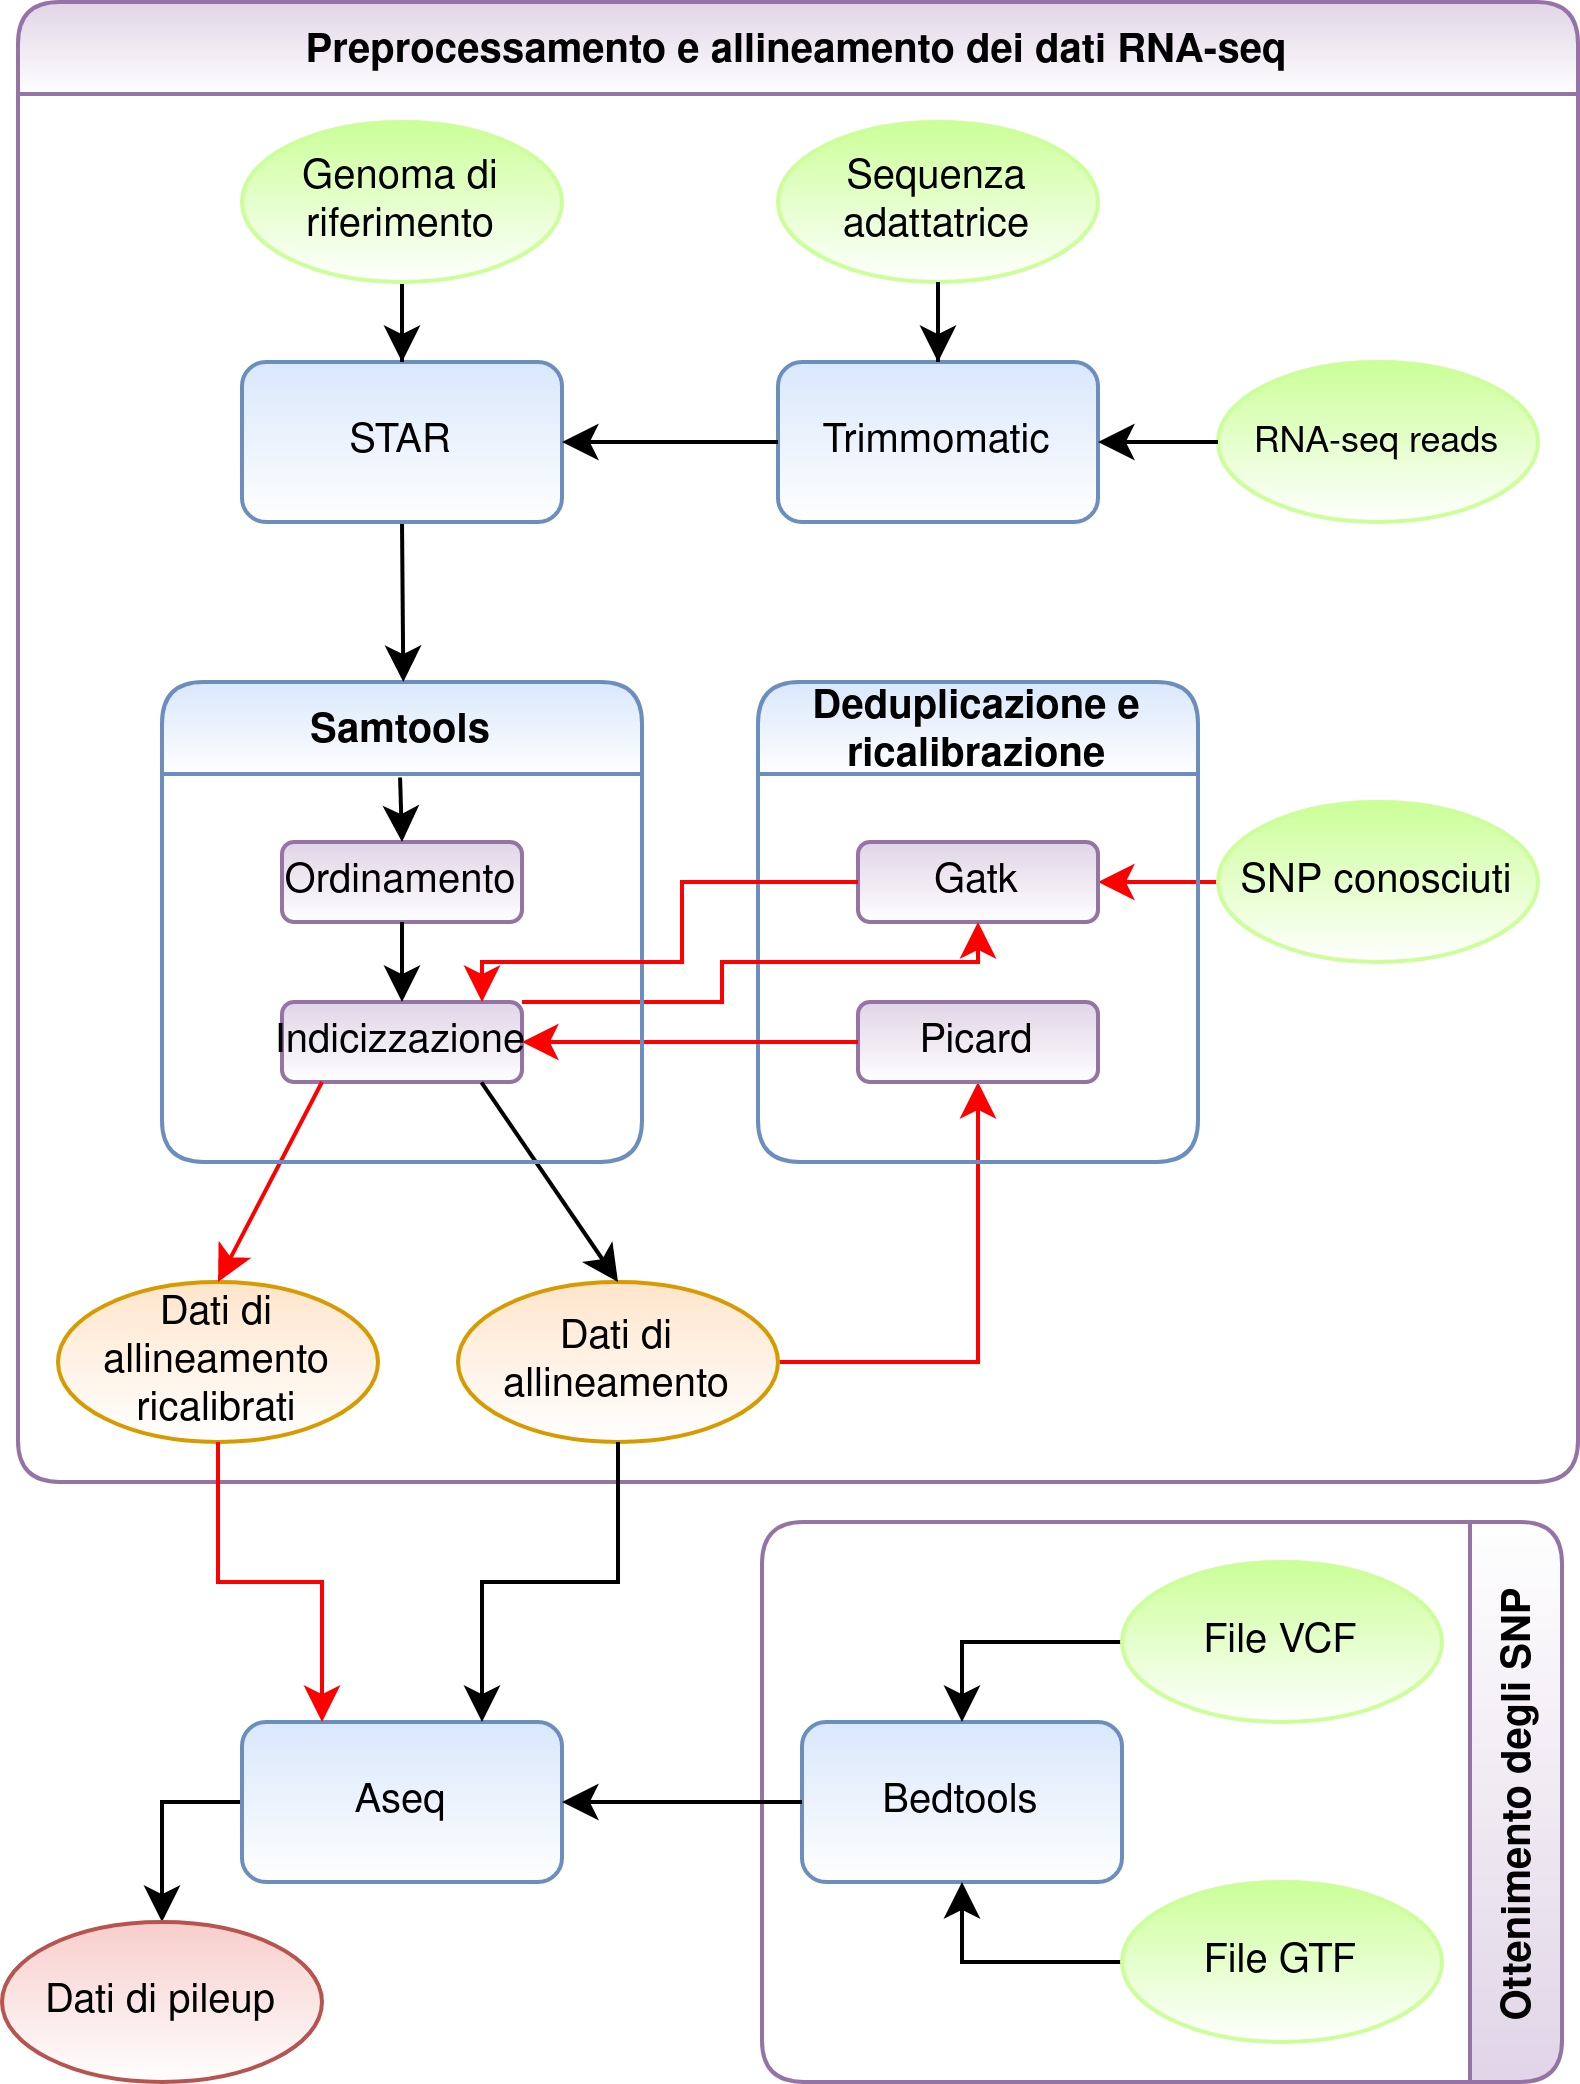
\includegraphics[scale=0.2]{pipeline.png}
    \caption{Pipeline per l'ottenimento dei dati di allelic imbalance}
  \end{figure}

  \section{Pre-processamento e allineamento dei dati RNA-seq}
  \label{sec:pre_all_rna_seq}
  Il primo passo della pipeline appenda definita \`e il pre-processamento e l'allineamento dei dati RNA-seq.
  L'input della pipeline sono dei file \emph{FASTQ}, ovvero file di testo che contengono i dati di sequenziamento raccolti in laboratorio tipicamente compressi.
  Questi file vengono modificati dai tool Trimmomatic, Star e Samtools in modo da produrre un output gi\`a utilizzabile per ottenere i dati di sbilanciamento allelico.
  Opzionalmente l'output pu\`o subire ulteriori modifiche prima di passare alla prossima fase: in particolare pu\`o essere deduplicato e ricalibrato.

  	\subsection{Trimmomatic}
	Trimmomatic \cite{trimmomatic} \`e il primo tool ad essere utilizzato.
	Il suo obiettivo \`e quello di eliminare dalle reads la sequenza adattatrice, o suoi frammenti, utilizzata per rendere possibile il sequenziamento.
	Essendo le RNA-seq fornite a single-ends\footnote{Punta a spiegazione nel capitolo 1} viene utilizzata la simple mode del tool.
	Questa scansiona ogni read\footnote{Non so se metterla in italiano} dalla terminazione $5'$ alla $3'$ per determinare la presenza della sequenza adattatrice.
	Utilizza il mdetodo ``seed and extend'' per trovare corrispondenze iniziali, anche non perfette, tra la read e la sequenza adattatrice.
	Successivamente svolge un allineamento locale e se questo ha uno score maggiore di una soglia viene rimosso insieme alla porzione successiva ad esso.
	Questa modalit\`a permette di identificare ogni sequenza adattatrice in ogni luogo della read a patto che l'allineamento sia abbastanza lungo e la read abbastanza accurata.
	Si nota per\`o come nelle regioni dove solo una corta corrispondenza parziale \`e possibile come alle estremit\`a della read e pertanto i contaminanti non possono essere identificati attendibilmente.
	Oltre alla rimozione delle sequenze adattatrici Trimmomatic tronca un'estremit\`a secondo un algoritmo di filtraggio secondo qualit\`a.
	Tra i metodi forniti dallo strumento \`e stato utilizzato quello del ``sliding window quality filtering'':
	scansiona la read dal $5'$ e rimuove la terminazione $3'$ quando la qualit\`a media di un gruppo di basi scende sotto una soglia specificata.
	Il risultato di questo passaggio sar\`a un altro fastq file con le sequenze adattatrici rimosse.

	\subsection{Star}
	\label{subsec:star}
	Star (spliced transcript alignment to a reference) \cite{star} \`e il secondo tool della pipeline.
	Prende come input il file fastq generato da Trimmomatic e un genoma di reference\footnote{Anche qui lo lascio in italiano?} e allineando il primo al secondo.
	Questo tool \`e stato creato con l'obiettivo di allineare RNA-seq di media-grande lunghezza, a differenza dei suoi competitori che, essendo creati a partire da allineatori per dati di DNA, hanno un maggiore tasso di errore.
	Questo avviene a causa degli eventi di splicing che avvengono nella creazione delle molecole di mRNA.
	Star pertanto si prefigge di permettere un allineamento accurato di reads che contengono mal-accoppiamenti, inserzioni o delezioni causati da variazioni genomiche o errori di sequenziamento mappando contemporaneamente sequenze derivate da regioni genomiche non contigue unite da eventi di splicing.
	Per farlo utilizza un algoritmo in due fasi.
	La prima fase o \emph{seed search} consiste della ricerca sequenziale di \emph{Maximal Mappable Prefix MMP}.
	Data una sequenza $R$, una regione $i$ e un genoma di reference $G$, $MMP(R, i, G)$ \`e la pi\`u lunga sottostringa $(R_i, R_{i+1}, \dots, R_{i+MMK-1})$ che corrisponde esattamente a una o pi\`u sottostringhe di $G$.
	$MML$ \`e la massima lunghezza mappabile.
	Questo permette un'identificazione di giunzioni di splicing senza nessuna conoscenza a priori.
	L'implementazione attraverso \emph{Uncompressed suffix arrays} causa alla complessit\`a dell'algoritmo di scalare logaritmicamente con la lunghezza del genoma di reference.
	Gli array sono non compressi per permettere tempi di ricerca pi\`u veloci, ma causano un aumento del consumo di memoria.
	La seconda fase o \emph{clustering, stitching and scoring} consiste nel costruire allineamenti dell'intera sequenza di reads unendo tutti i seed allineati al genoma nella prima fase.
	In primo luogo i seed sono raggruppati insieme secondo la vicinanza a un seed ancora selezionato limitando il numero di loci genomici a cui questo si allinea.
	Successivamente tutti i seed mappati nella \emph{genomic window} sono uniti insieme assumendo un modello lineare locale di trascrizione.
	Questo processo di unione viene inoltre guidato da un sistema di punteggi che penalizza mal-accoppiamenti, inserzioni, delezioni e \emph{splice junction gap}.
	Star ha come output un sam file, un file di testo delimitato da tabulazioni contenente una riga per allineamento con tutte le informazioni necessarie per la sua identificazione.

	\subsection{Samtools}
	I samtools \cite{samtools} sono un insieme di programmi necessari per interagire con i dati di sequenziamento.
	Nella pipeline sono utilizzati per compiere delle operazioni sui sam file generati da Star\footnote{Vedi \S\ref{subsec:star}} in modo da prepararli prima che possano essere utilizzati successivamente per generare i dati di sbilanciamento allelico\footnote{Vedi \S\ref{sec:aseq}}.
  In particolare svolgono le operazioni di ordinamento, indicizzazione e compressione dei file di input.
  Questo avviene attraverso due programmi: samtools sort \cite{samtools-sort} e samtools index \cite{samtools-index}.
  Il primo ordina gli allineamenti secondo le coordinate di inizio e comprime implicitamente l'input in formato bam.
  Il secondo invece crea, a partire dall'output del programma sort un indice in formato bai di tale file, permettendo efficienti operazioni di accesso casuale al bam file.
  L'output finale \`e un bam file ordinato e indicizzato che pu\`o essere utilizzato come input di aseq.

	\subsection{Deduplicazione e ricalibrazione}
        \label{subsec:deduprecab}
	La deduplicazione e la ricalibrazione sono due processi ulteriori di pre-processamento dei dati che tentano di risolvere errori presenti nei bam file che sono stati allineati attraverso star\footnote{Vedi \S\ref{subsec:star}}.
  Questi due passaggi vengono svolti attraverso una serie di tools eseguiti sequenzialmente come si nota nella figura \ref{fig:pipeline_deduprecal}.
  \begin{figure}[H]
    \label{fig:pipeline_deduprecal}
    \centering
    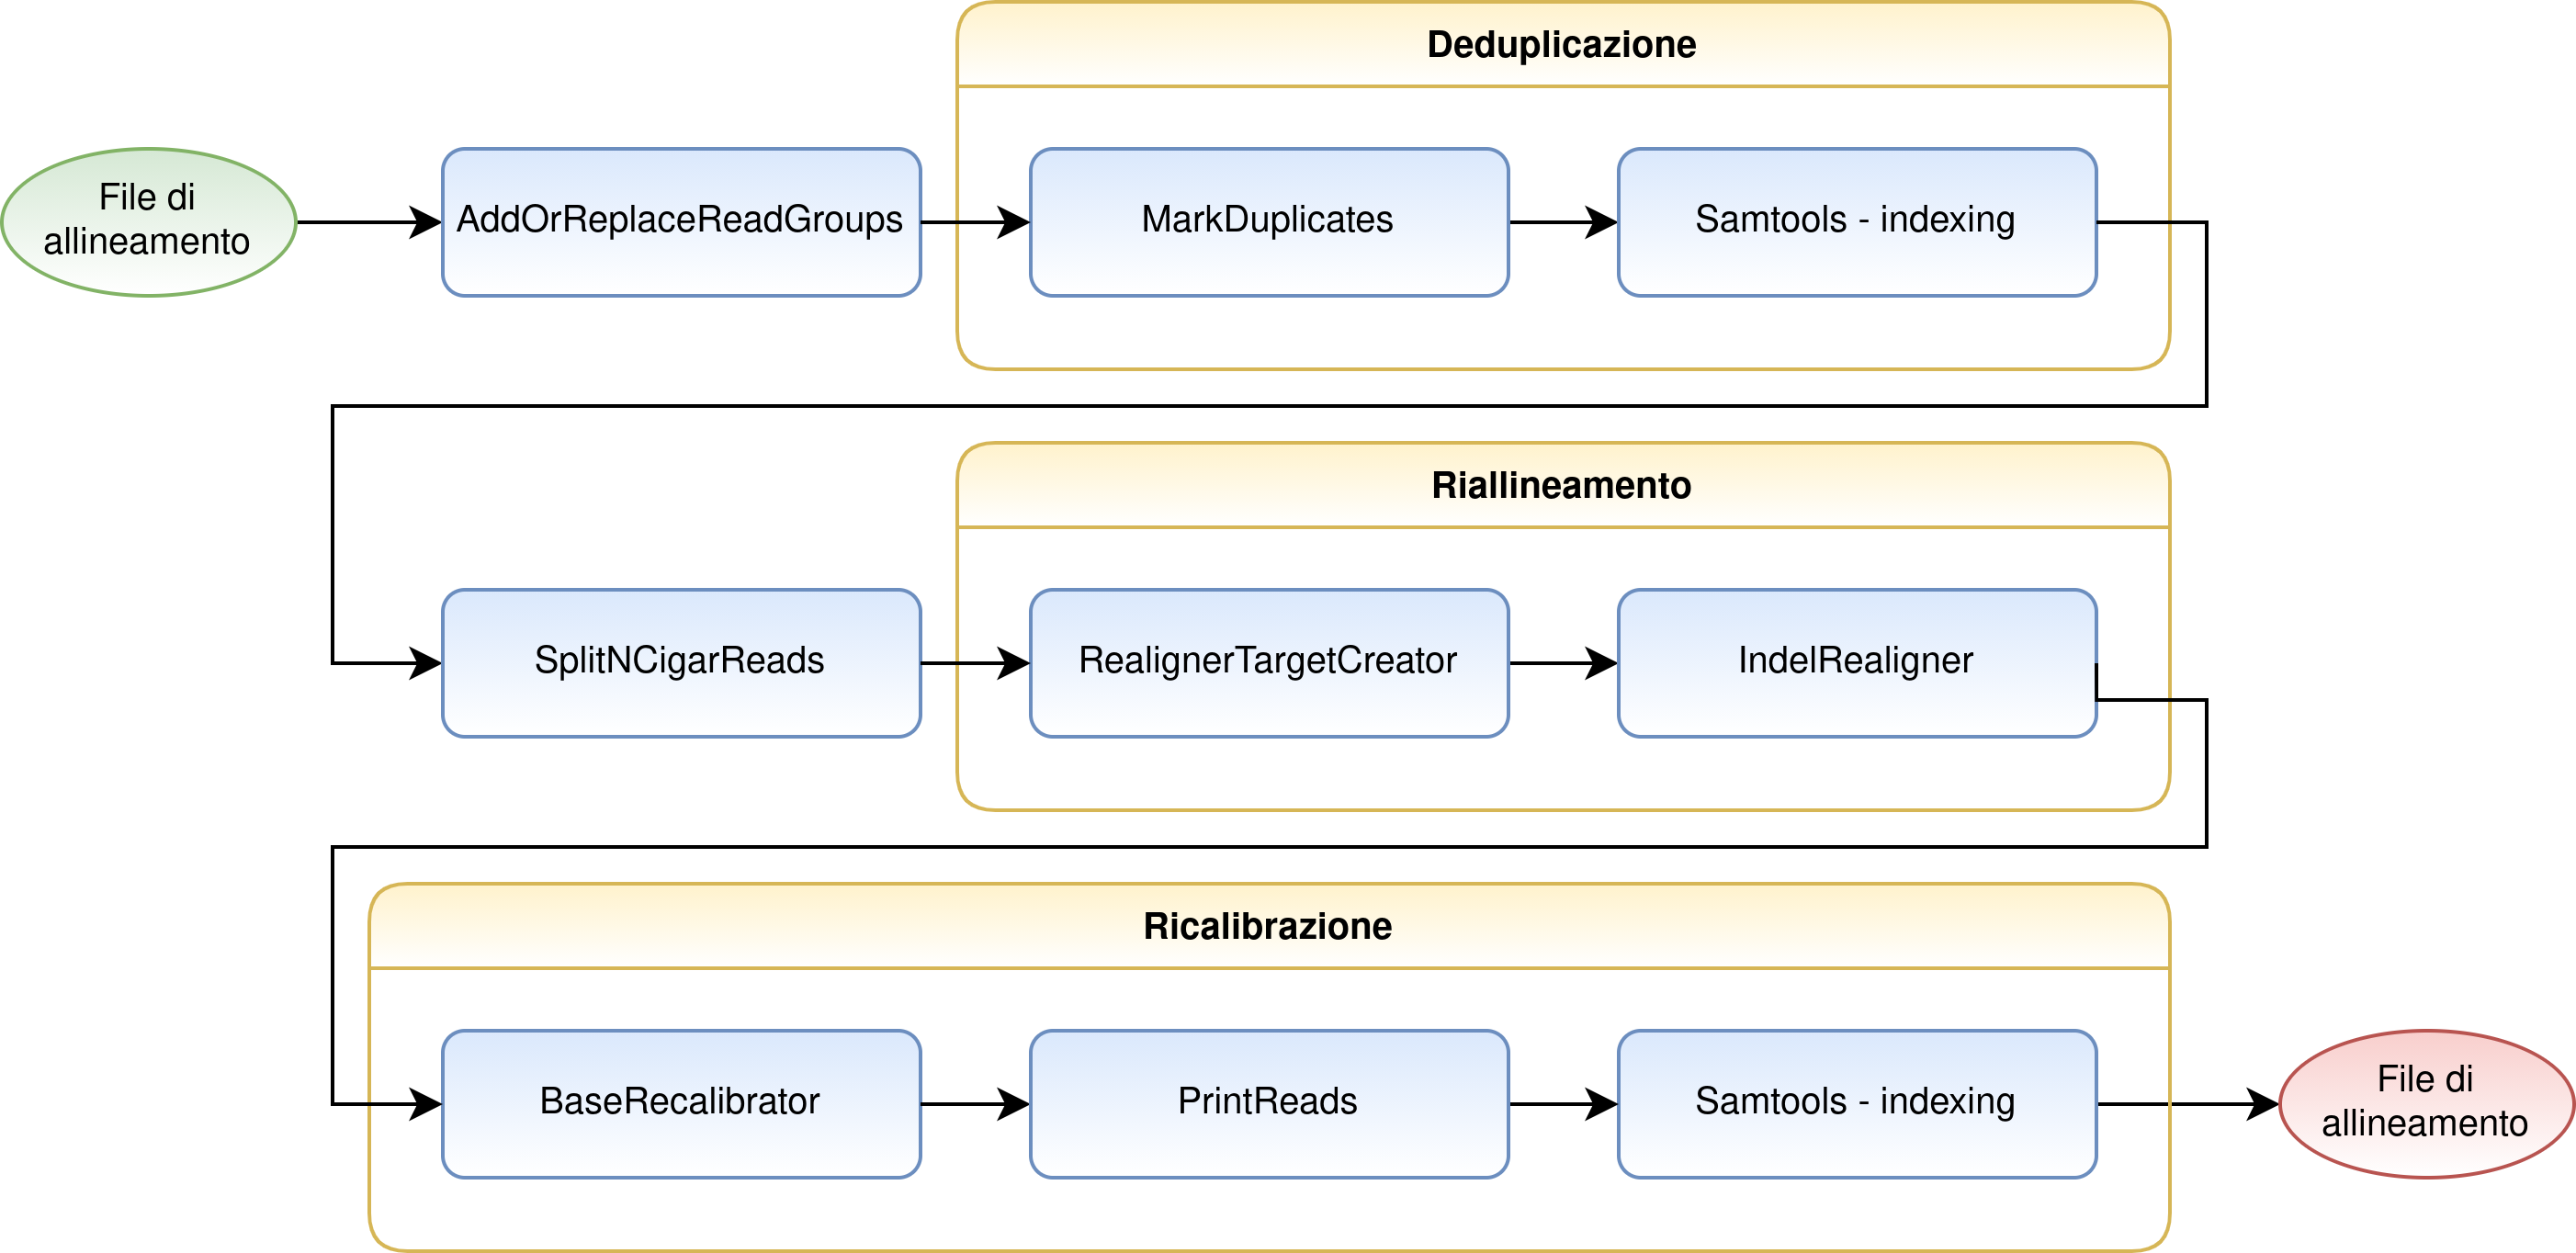
\includegraphics[scale=0.17]{deduprecal.png}
    \caption{Pipeline di deduplicazione e ricalibrazione}
  \end{figure}
  Come si nota il primo passaggio viene svolto dal tool \emph{AddOrReplaceReadGroups} di Picard\cite{picard}, un passaggio di preparazione delle read necessario a tutti i tool successivi.
  Questo assegna tutte le reads in un file a un nuovo read-group settando un campo nel BAM file, in modo da assegnare tutte le reads a un genotipo specifico.


    \subsubsection{Deduplicazione}
    Si definiscono come read duplicate in un BAM file delle read che si generano da un singolo frammento di RNA.
    Possono originarsi durante la preparazione del campione, per esempio durante la costruzione della libreria attraverso PCR o risultare da un singolo cluster di amplificazione, identificato incorrettamente come cluster multipli dal sensore ottico dello strumento di sequenziamento.
    Il processo di deduplicazione \`e stato svolto attraverso il \emph{MarkDuplicates} di Picard.
    Il programma compara le sequenze nelle posizioni $5'$ sia delle reads che dei read-pairs.
    Dopo che ha trovato tutti le reads duplicata queste vengono ordinate secondo la somma dei punteggi di qualit\`a delle basi.
    La read con il punteggio pi\`u alto viene considerata primaria, le altre duplicati.
    Grazie all'opzione \emph{REMOVE\_DUPLICATE=true} tutte le sequenze duplicate vengono rimosse.
    Viene infine ricreato l'indice del BAM file attraverso \emph{samtools index}.

    \subsubsection{Ricalibrazione}
    La ricalibrazione viene svolta da una serie di tool facenti parte della suite Gatk \cite{gatk}.
    Il processo si compone di diverse fasi:
    \begin{multicols}{2}
      \begin{enumerate}
        \item Riallineamento degli indels.
        \item Ricalibrazione delle basi basata sul punteggio di qualtit\`a.
      \end{enumerate}
    \end{multicols}
    Il primo passaggio, svolto dal tool \emph{SplitNCigarReads}, progettato specificatamente per dati di RNA-seq \`e necessario per il corretto funzionamento degli step successivi.
    In un file BAM di RNA-seq infatti si trovano stringhe \emph{CIGAR} che descrivono come una base in ogni reads \`e mappata.
    Il valore $N$ corrisponde a una base saltata sul genoma di reference\footnote{Probabilmente in italiano}.
    Nel caso di RNA-seq tali basi possono corrispondere o a sequence introniche, non presenti nel RNA a causa dello splicing o a sequenze di ``overhang''\footnote{Magari una definizione di overhang}.
    \emph{SplitNCigarReads} elimina le basi corrispondenti a una $N$ creando dalla reads di partenza due reads, una a sinistra e una a destra della base rimossa.
    Come risultato gli esoni del RNA vengono separati in segmenti e gli overhang eliminati in modo da non causare falsi positivi.\\
    Dopo questo lavoro di processamento inizia la fase di riallineamento degli indels.
    Il riallineamento locale degli indels \`e necessario in quanto permette di correggere errori generati dall'allineatore genomico.
    Questi errori si generano in quanto gli allineatori genomici considerano ogni read indipendentemente e le strategie di assegnazione dei punteggi limitano la loro abilit\`a di allineare accuratamente nella presenza di indels.
    Il processo di allineamento locale considera invece tutte le letture che attraversano una posizione in modo da ottenere un consenso di alto punteggio che supporta la presenza di un evento di indel.
    Il riallineamento viene svolto attraverso l'utilizzo di due tool: \emph{RealignerTargetCreator} e \emph{IndelRealigner}.
    Il primo prende come input un BAM file ordinato e indicizzato.
    A partire dal file genera un file di output formato da una lista a una colonna contenente gli intervalli, che rappresentano siti di indel potenziali
    Se sono prossimali i siti sono uniti in un intervallo unico.
    Il secondo prende come input lo stesso BAM di \emph{RealignerTargetCreator} e il file di intervalli appena generato e svolge un riallineamento locale sulle reads coincidenti con l'intervallo target usando consensi dagli indel presenti nell'allineamento originale.
    L'output \`e un BAM ordinato e indicizzato.\\
    Il processo di ricalibrazione delle basi basato sul punteggio di qualit\`a serve a risolvere errori generati durante il sequenziamento.
    Si definisce il punteggio di qualit\`a di una base come una stime dell'errore emesso dalla macchina di sequenziamento: esprimono quanto questa \`e confidente che ha chiamato la base corretta ogni volta.
    Questi punteggi sono soggetti a varie sorgenti di errori tecnici dovuti alla fisica o alla chimica di come una reazione di sequenziamento funziona o a difetti nell'equipaggiamento.
    Gli errori portano pertanto a una sottostima o sovrastima (tipicamente la seconda) del punteggio di qualit\`a fornito dal macchinario di sequenziamento.
    Per tentare di risolvere si utilizza machine learning per modellarli empiricamente a modificare i valori di qualit\`a migliorarne la veridicit\`a.
    La ricalibrazione delle basi avviene attraverso l'utilizzo di due tool.
    Il primo \emph{BaseRecalibrator} costruisce un modello di covarianza da un BAM e da un insieme di varianti conosciute in un file VCF e lo salva in un file.
    Le varianti conosciute sono usate per mascherare basi ai siti di variazioni aspettate in modo da non considerarle come errori.
    Al di fuori di queste eccezioni ogni mal-accoppiamento viene contato come un errore.
    Per costruire il modello di ricalibrazione il tool tabula i dati del BAM secondo il read group, il punteggio di qualit\`a, il ciclo della macchina che ha prodotto la base, la base corrente e successiva.
    Successivamente si conta il numero di basi e quanto spesso queste hanno un mal-accoppiamento con la base di reference.
    Il secondo tool \emph{PrintReads} applica il modello creato dal primo al BAM di input, aggiornando cos\`i ai punteggi di qualit\`a migliorati.
    Infine viene ricreato l'indice del BAM file attraverso \emph{samtools index}.\\
    In questo modo si \`e creato un file BAN pronto per essere utilizzato da ASEQ.

  \section{Ottenimento degli SNP di interesse}
  Una volta ottenuti i file di allineamento si rende necessario ottenere una lista di SNP dei quali si vuole ottenere il valore di sbilanciamento allelico.
  Per ottenere questi dati sono stati utilizzati un file GTF ottenuto da\footnote{Mettere da dove si \`e ottenuto} contenente informazioni sulla porzione esonica del genoma umano e da un insieme di VCF divisi per cromosoma contenenti le informazioni riguardo le varianti ottenute negli essere umani.
  Dopo aver ristretto i VCF agli SNP sono stati intersecati con il file GTF.
  L'intersezione \`e stata volta dal tool \emph{bedtools intersect}, facente parte della suite bedtools\footnote{Inserisci sito}.
  Questo tool ha permesso di trovare ogni record del VCF presente anche nel GTF.
  In questo modo \`e stato creato un insieme di file VCF, uno per ogni cromosoma, contenente ogni SNP presente nella parte esonica del genoma.
  La restrizione alla parte esonica del genoma non causa alcuna perdita di potere predittivo in quanto si stanno considerando dati di RNA-seq e permette una significativa diminuzione del carico computazionale svolto da aseq\emph{riferimento ad aseq}.
  I VCF risultanti da questo processo sono pronti per essere utilizzati come input di aseq\footnote{riferimento ad aseq}.

  \section{Calcolo dei dati di sbilanciamento allelico}
  \label{sec:aseq}
  Per computare i valori di sbilanciamento allelico \`e stato utilizzato aseq \cite{aseq}.
  Questo tool tenta di risolvere alcune limitazioni di altri programmi di analisi di espressione allelo-specifica.
  Non richiede infatti informazioni genomiche dei genitori dell'individuo e non si basa unicamente sui dati di RNA-seq.
  Aseq in particolare utilizza dati di sequenziamento di prossima generazione trascrittomici e genomici accoppiati per superare queste limitazioni.
  \`E stato implementato sfruttando l'API di samtools, permettendo rapide funzionalit\`a di accesso casuale su file di allineamento indicizzati, combinandolo con il potere di computazione multi-threaded.
  Delle modalit\`a che aseq fornisce \`e stata utilizzata quella principale di analisi ASE, ponendo limitazioni solo sulla qualit\`a delle basi e la qualit\`a delle letture dei file di allineamento in modo da computare i dati di pileup per tutti gli SNP trovati nel file.
  Questo permette di applicare diversi tipi di soglie in un secondo momento, evitando di computare continuamente i dati di pileup.
  Non si sfrutta pertanto il potere di individuazione di eventi di ASE da parte di aseq, ma si sfrutta unicamente il suo veloce engine computazionale che permette di ridurre il carico computazionale della creazione dei dati di pileup per una singola base.
  Pertanto, una volta prodotti i file di allineamento dai dati di RNA-seq e la lista di SNP esonici si procede all'esecuzione di aseq.
  In particolare i file di allineamento sono divisi in due insiemi: uno creato dopo l'allineamento con star\footnote{Vedi\S\ref{subse:star}} e l'altro dopo il processo di deduplicazione e ricalibrazione\footnote{Vedi \S\ref{subsec:deduprecab}}.
  Ognuno di questi insiemi possiede un file per campione\footnote{Riferimento a lista di campioni}.
  La lista di SNP si trova invece in un insieme di file VCF, un file per ogni autosoma, uno per il cromosoma $X$ e uno per il DNA mitocondriale.
  Perci\`o per ogni file di allineamento viene eseguito aseq per ogni file VCF, ottenendo in questo modo i dati di pileup di ogni SNP per ogni campione divisi per cromosoma.
  L'output di aseq \`e un file di testo delimitato da tabulazioni, formato che rende facilmente ottimizzabili le successive analisi attraverso tool come awk, sed o framework come pandas per python o tidyverse per R.
  

      \newpage
      \graphicspath{{chapters/04/media/}}
\chapter{Analisi dei dati}
\label{cha:analisi}
%  \begin{figure}[H]
%    \centering
%    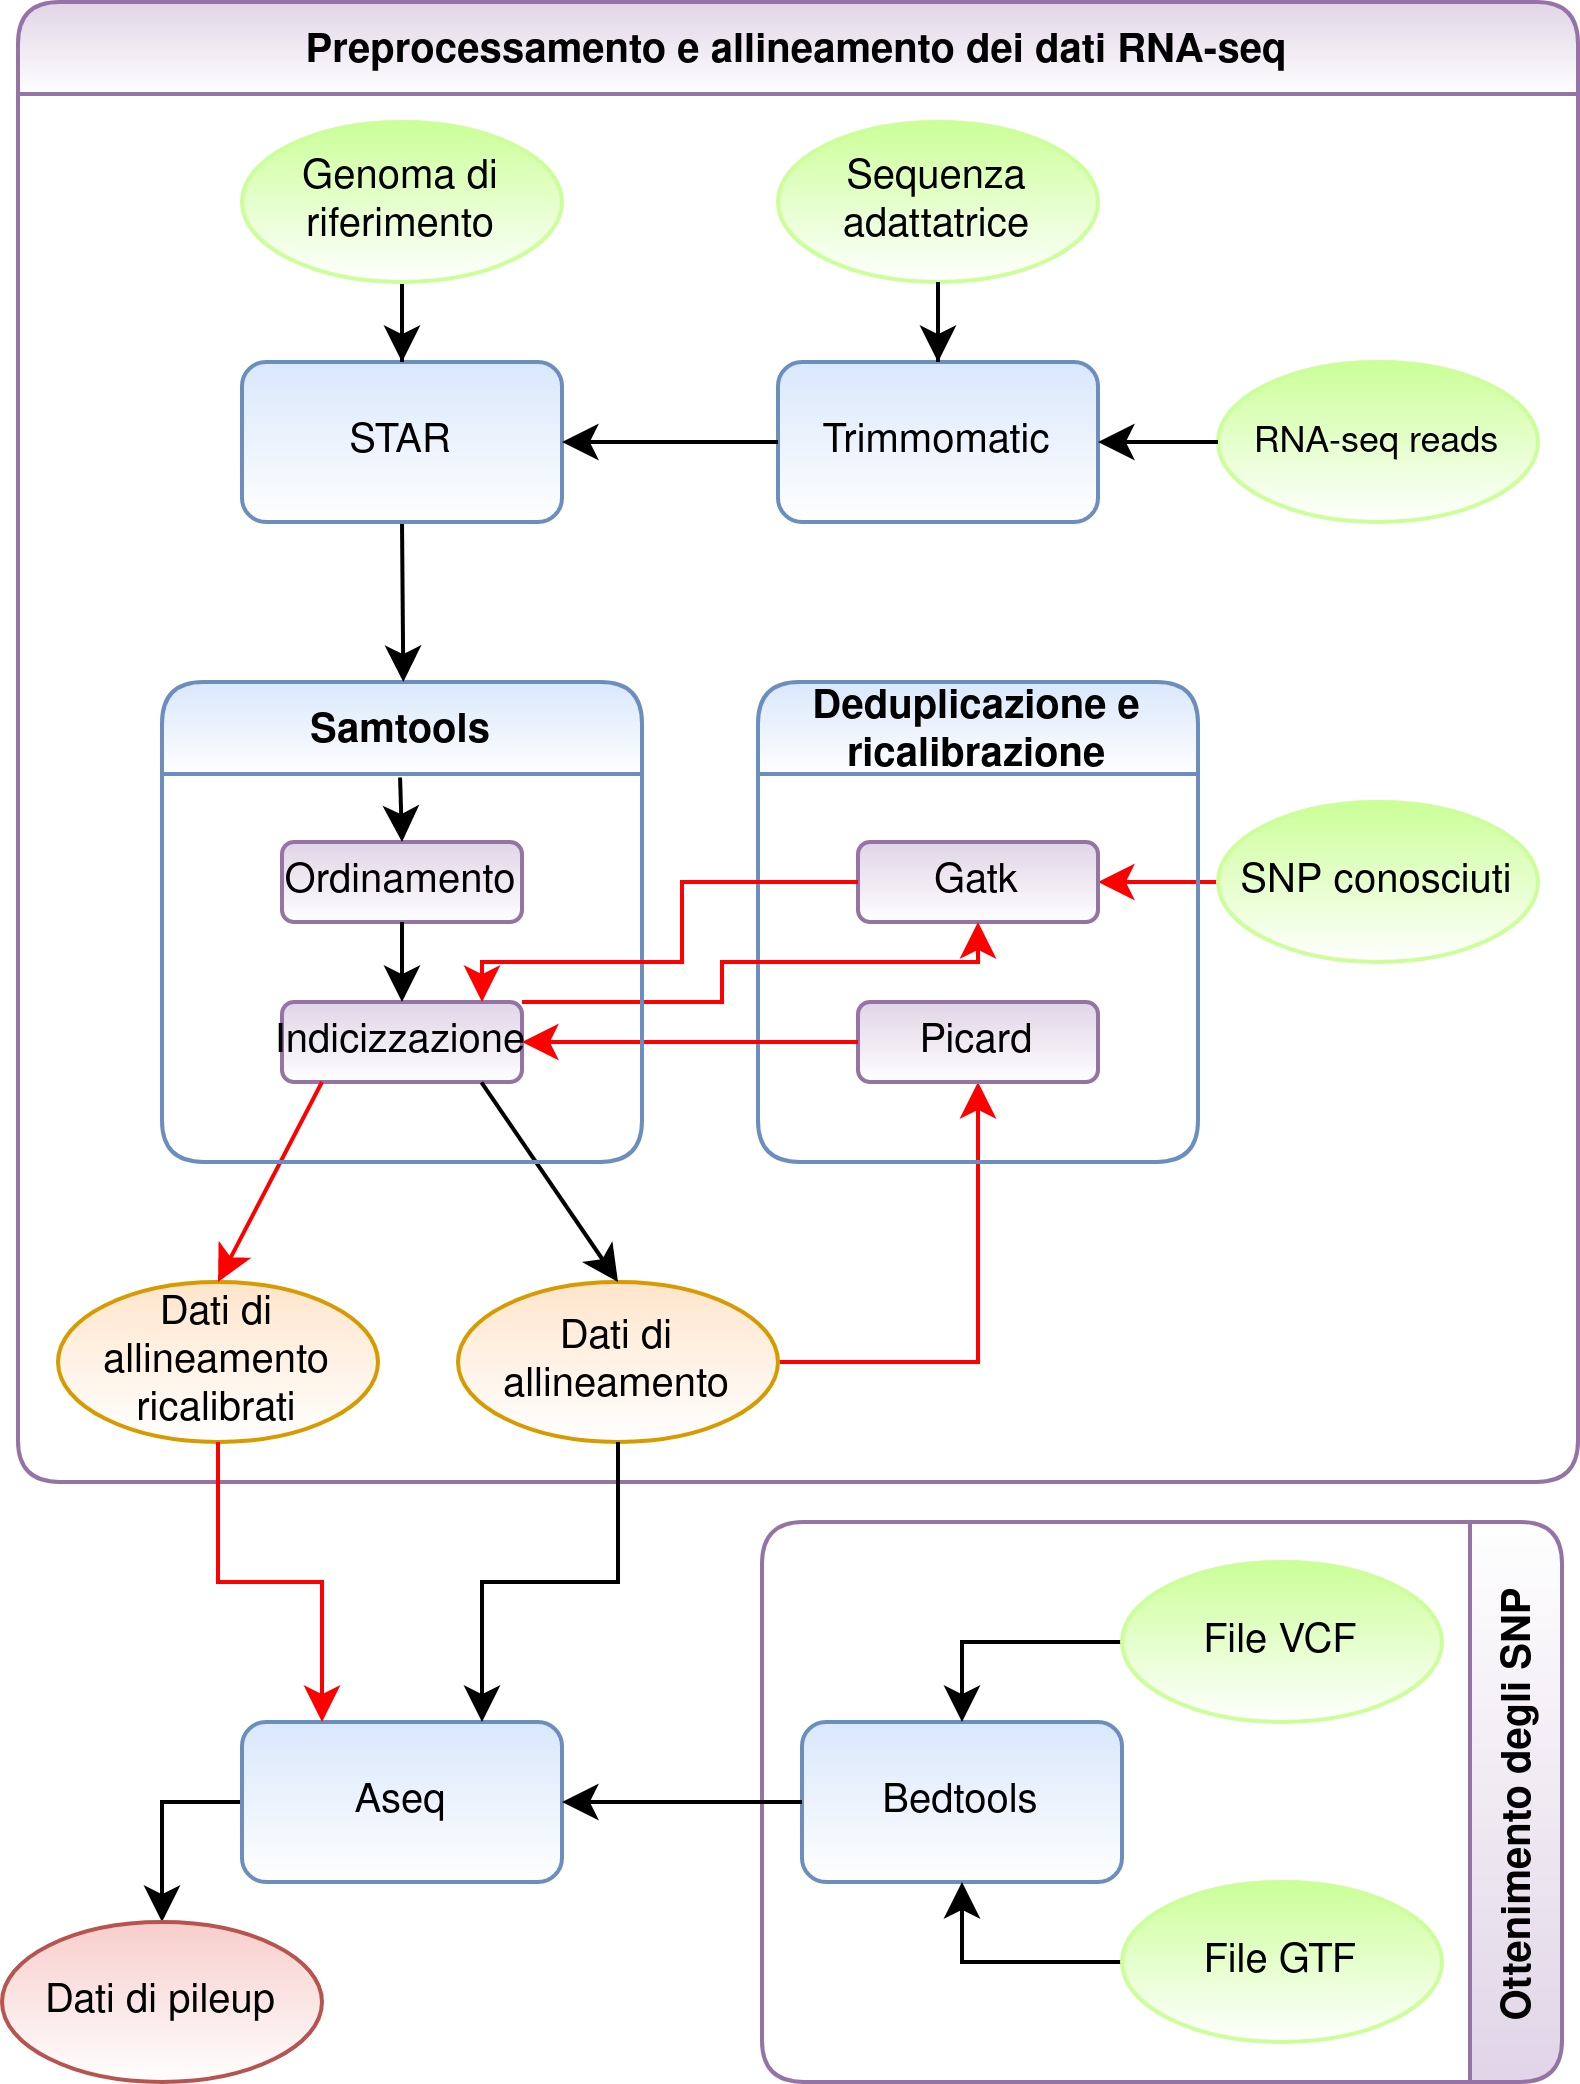
\includegraphics[scale=0.2]{pipeline.png}
%    \caption{Pipeline per l'ottenimento dei dati di allelic imbalance}
%    \label{fig:}
%  \end{figure}

\section{Identificazione delle varianti}

 \begin{figure}[H]
   \centering
   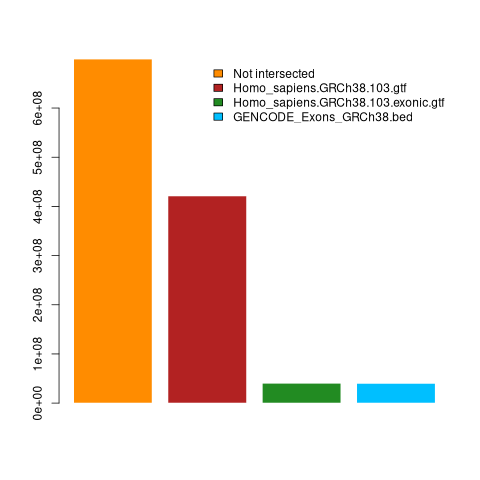
\includegraphics[scale=1]{scelta_gtf.png}
   \caption{SNP mantenuti dopo l'intersezione con i VCF}
   \label{fig:}
 \end{figure}

\section{Conta degli SNP trovati con ASEQ}
\label{sec:snp_count}
 \begin{figure}[H]
   \centering
   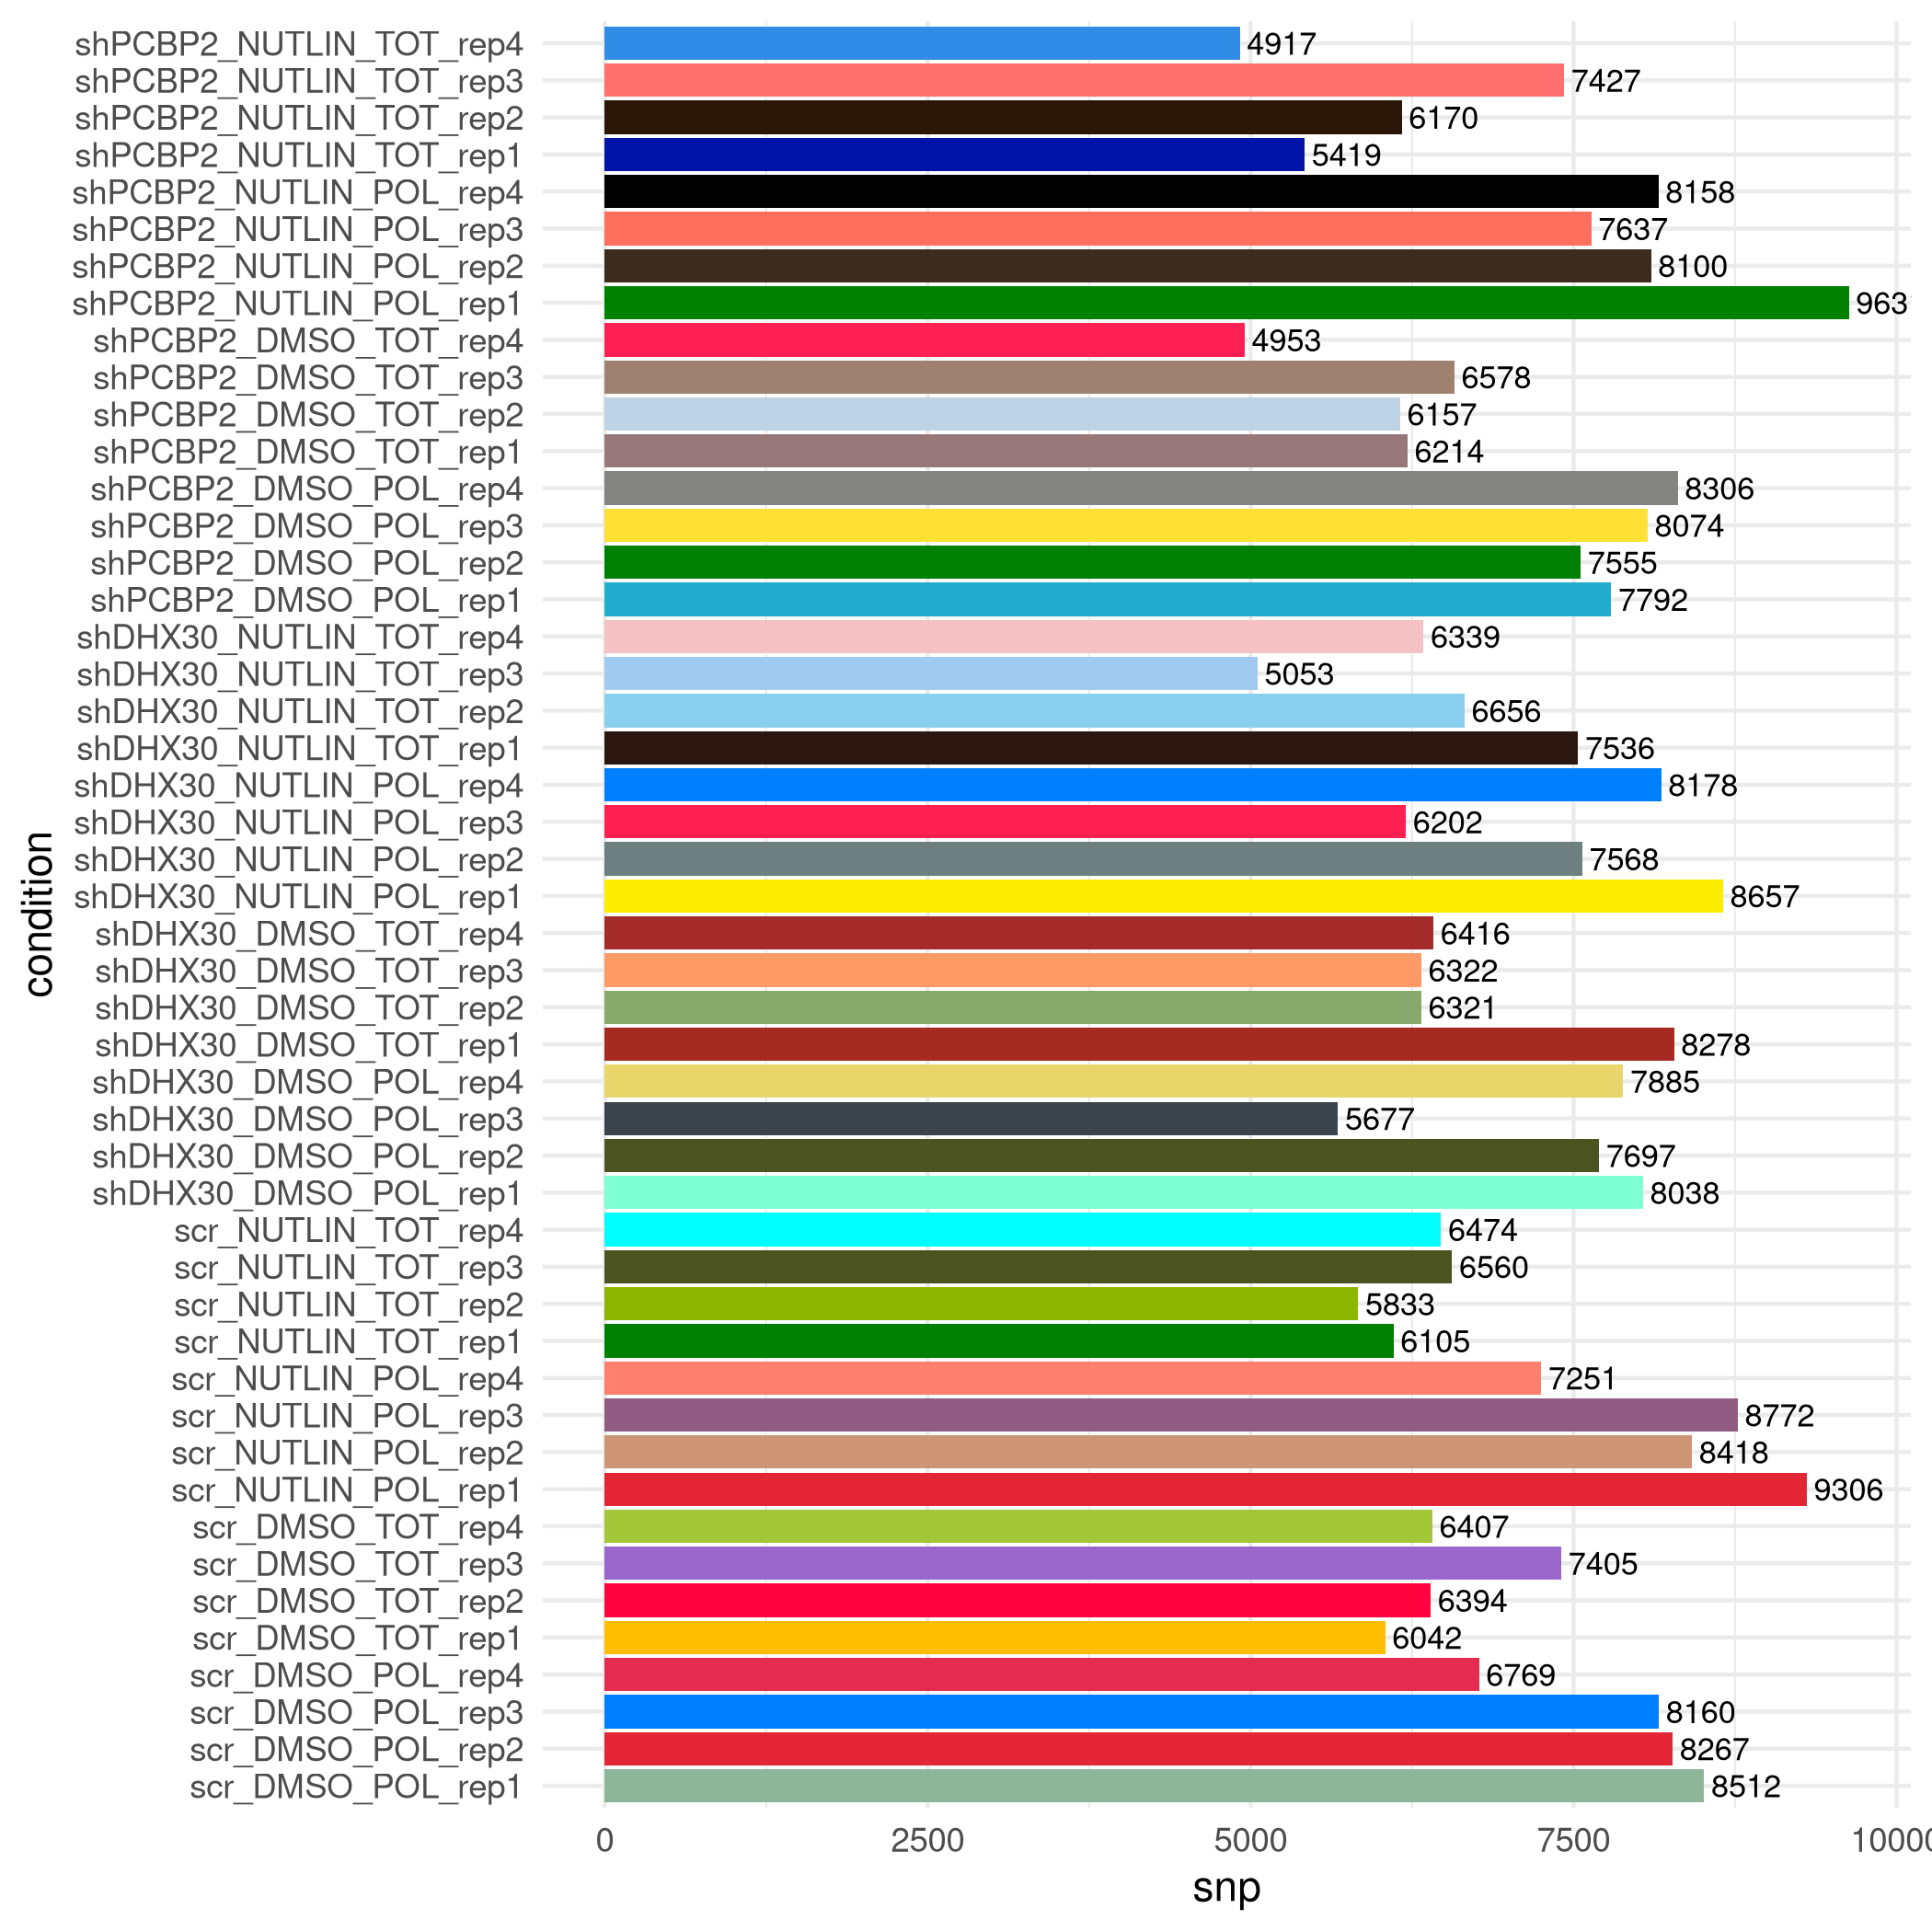
\includegraphics[scale=1]{aseq_count_2_8_10_pre.png}
	 \caption{Conta per campione degli SNP eterozigoti trovati con aseq ($0.2< af < 0.8$ e coverage $\ge 10$)}
   \label{fig:}
 \end{figure}

 \subsection{Distrubuzione degli SNP}
 \begin{figure}[H]
   \centering
   \begin{tabular}{ccc}
      \subfloat[scr DMSO]{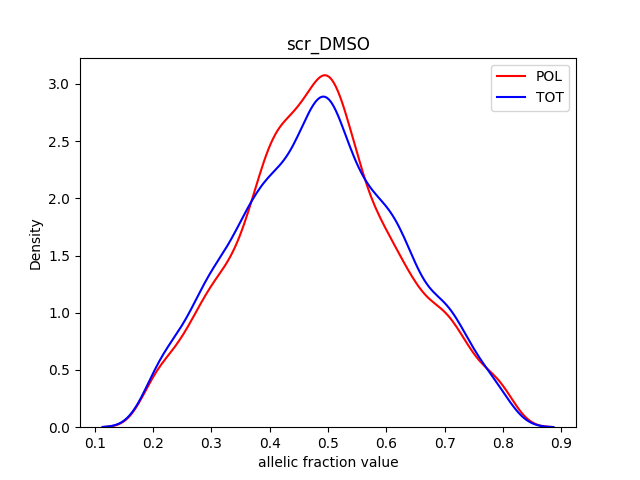
\includegraphics[width = 0.3\textwidth]{distribution/scr_DMSO.png}} &
      \subfloat[scr NUTLIN]{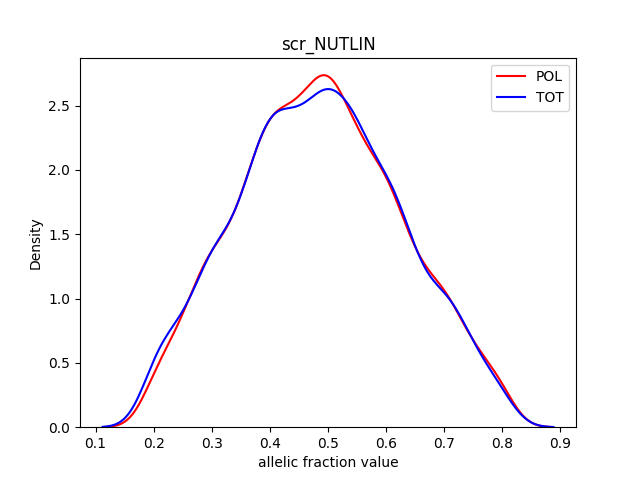
\includegraphics[width = 0.3\textwidth]{distribution/scr_NUTLIN.png}} &
      \subfloat[shDHX30 DMSO]{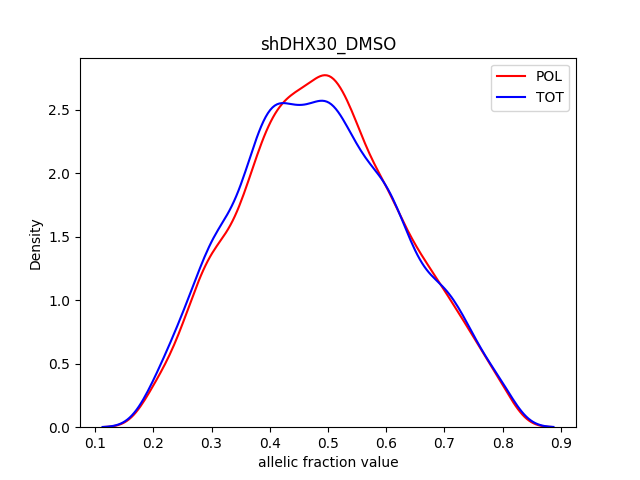
\includegraphics[width = 0.3\textwidth]{distribution/shDHX30_DMSO.png}} \\
      \subfloat[shDHX30 NUTLIN]{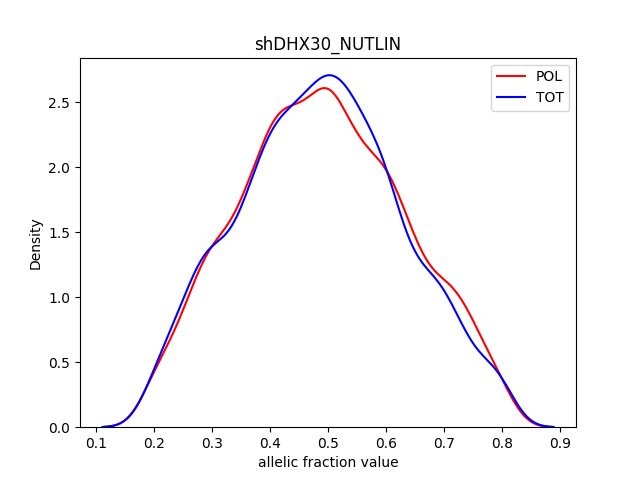
\includegraphics[width = 0.3\textwidth]{distribution/shDHX30_NUTLIN.png}} &
      \subfloat[shPCBP2 DMSO]{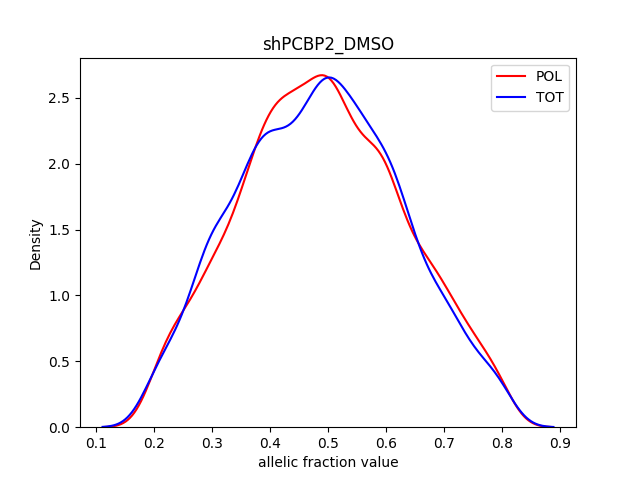
\includegraphics[width = 0.3\textwidth]{distribution/shPCBP2_DMSO.png}} &
      \subfloat[shPCBP2 NUTLIN]{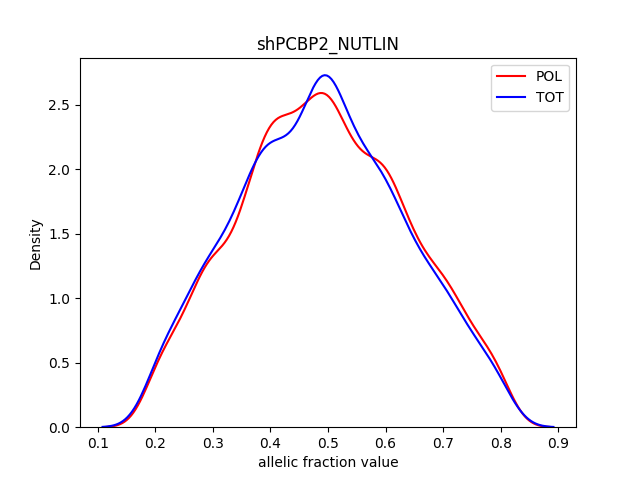
\includegraphics[width = 0.3\textwidth]{distribution/shPCBP2_NUTLIN.png}} \\
  \end{tabular}
   \label{fig:}
 \end{figure}

\section{Qualit\`a dei campioni}
Confronto tra replicato di un campione in modo da verificare come cambiano i valori di AF tra un replicato e l'altro.
 \begin{figure}[H]
   \centering
   \begin{tabular}{ccc}
      \subfloat[1 - 2]{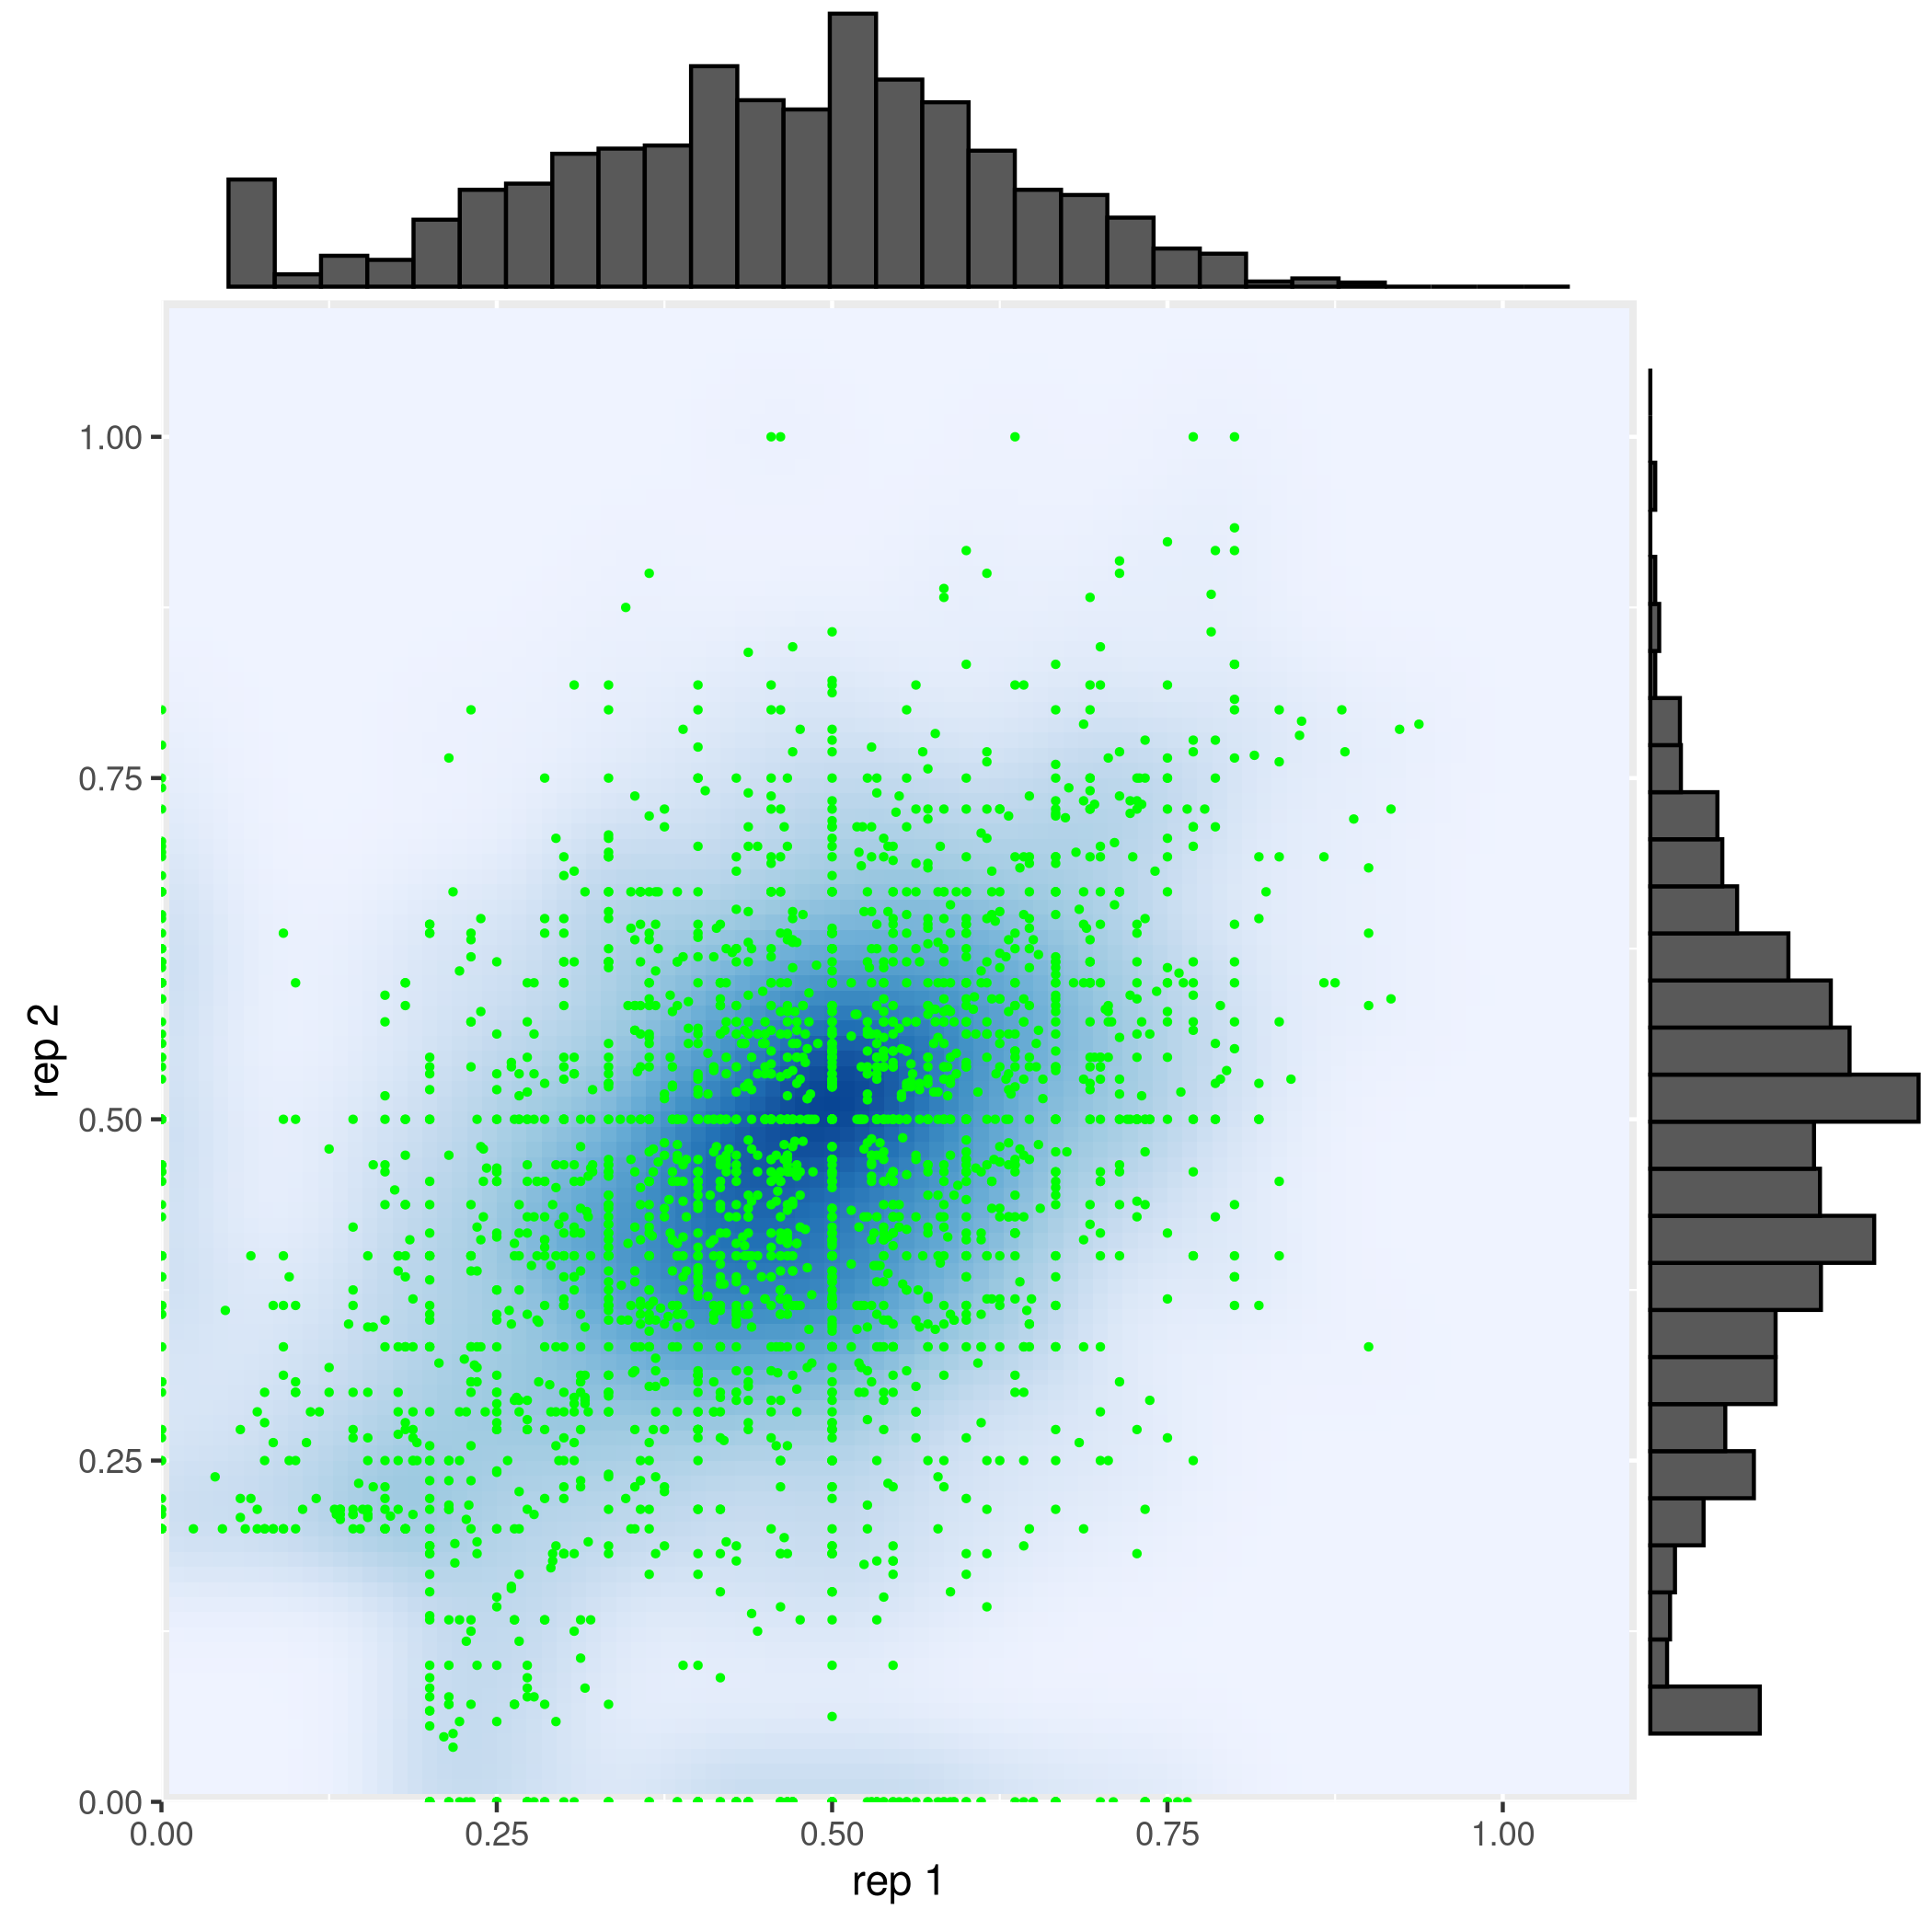
\includegraphics[width = 0.3\textwidth]{rep_corr/scr_DMSO_TOT-rep-1-2.post.0.2.0.8.10.png}} &
      \subfloat[1 - 3]{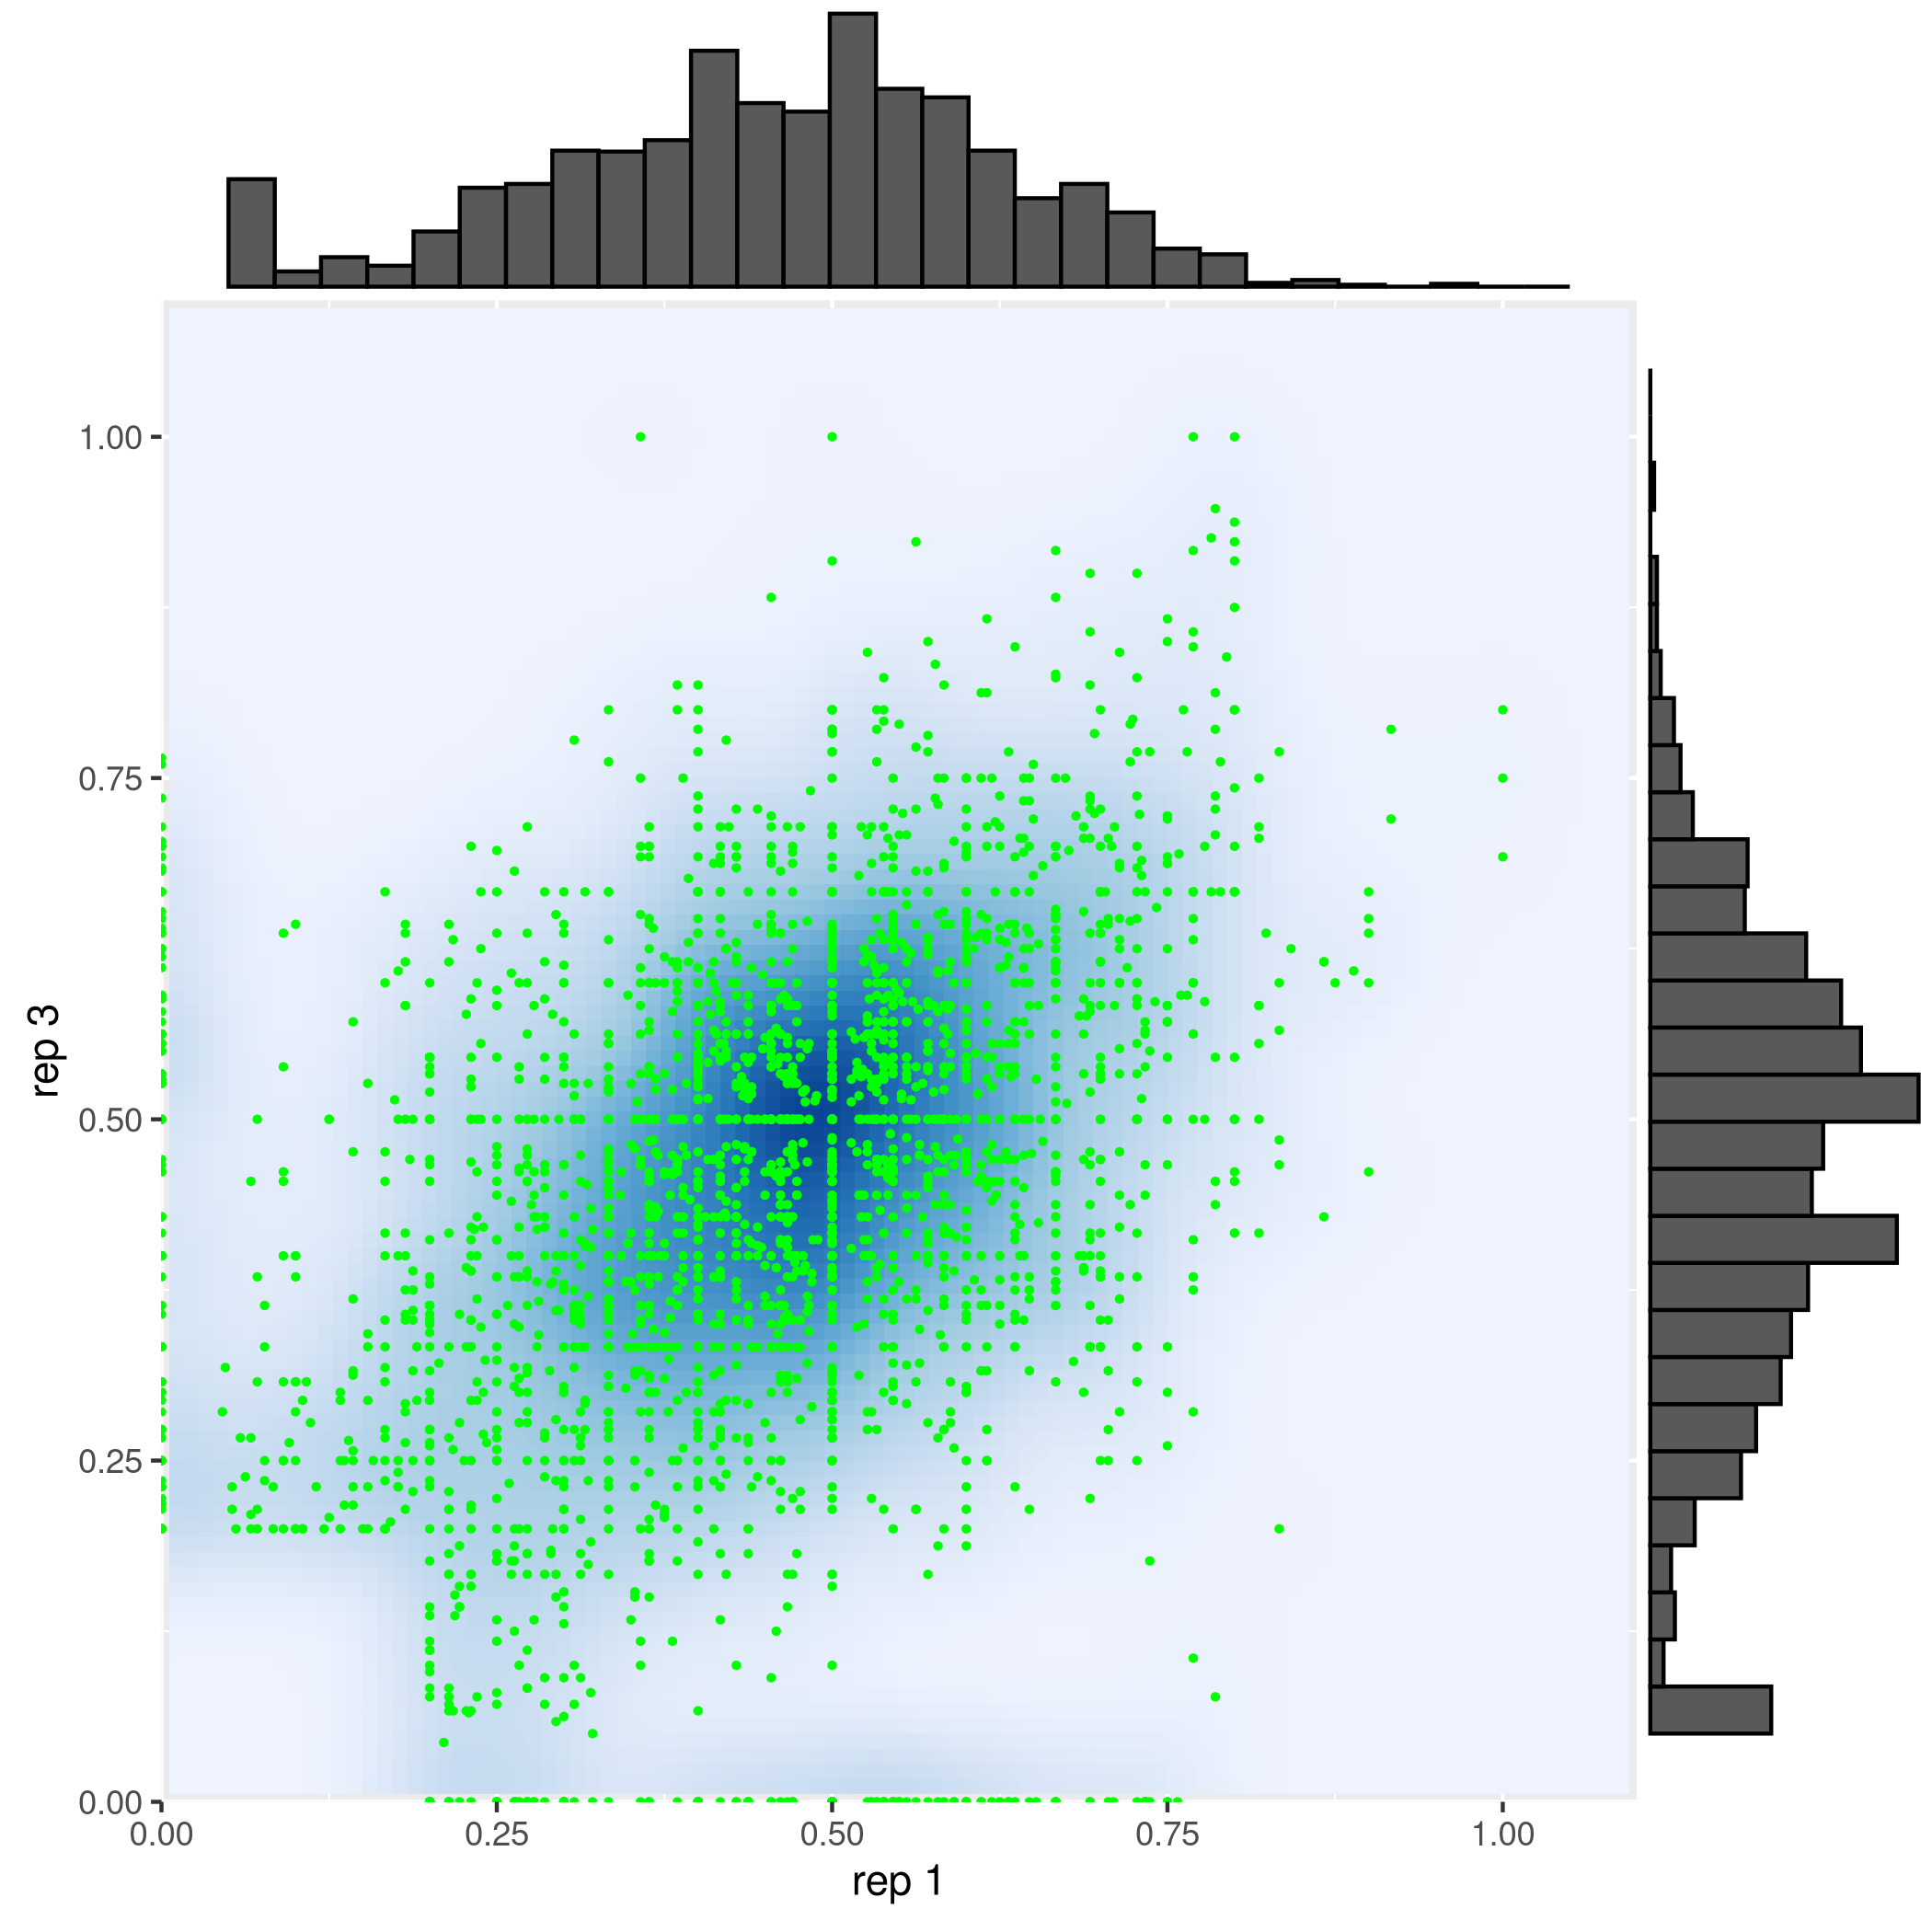
\includegraphics[width = 0.3\textwidth]{rep_corr/scr_DMSO_TOT-rep-1-3.post.0.2.0.8.10.png}} &
      \subfloat[1 - 4]{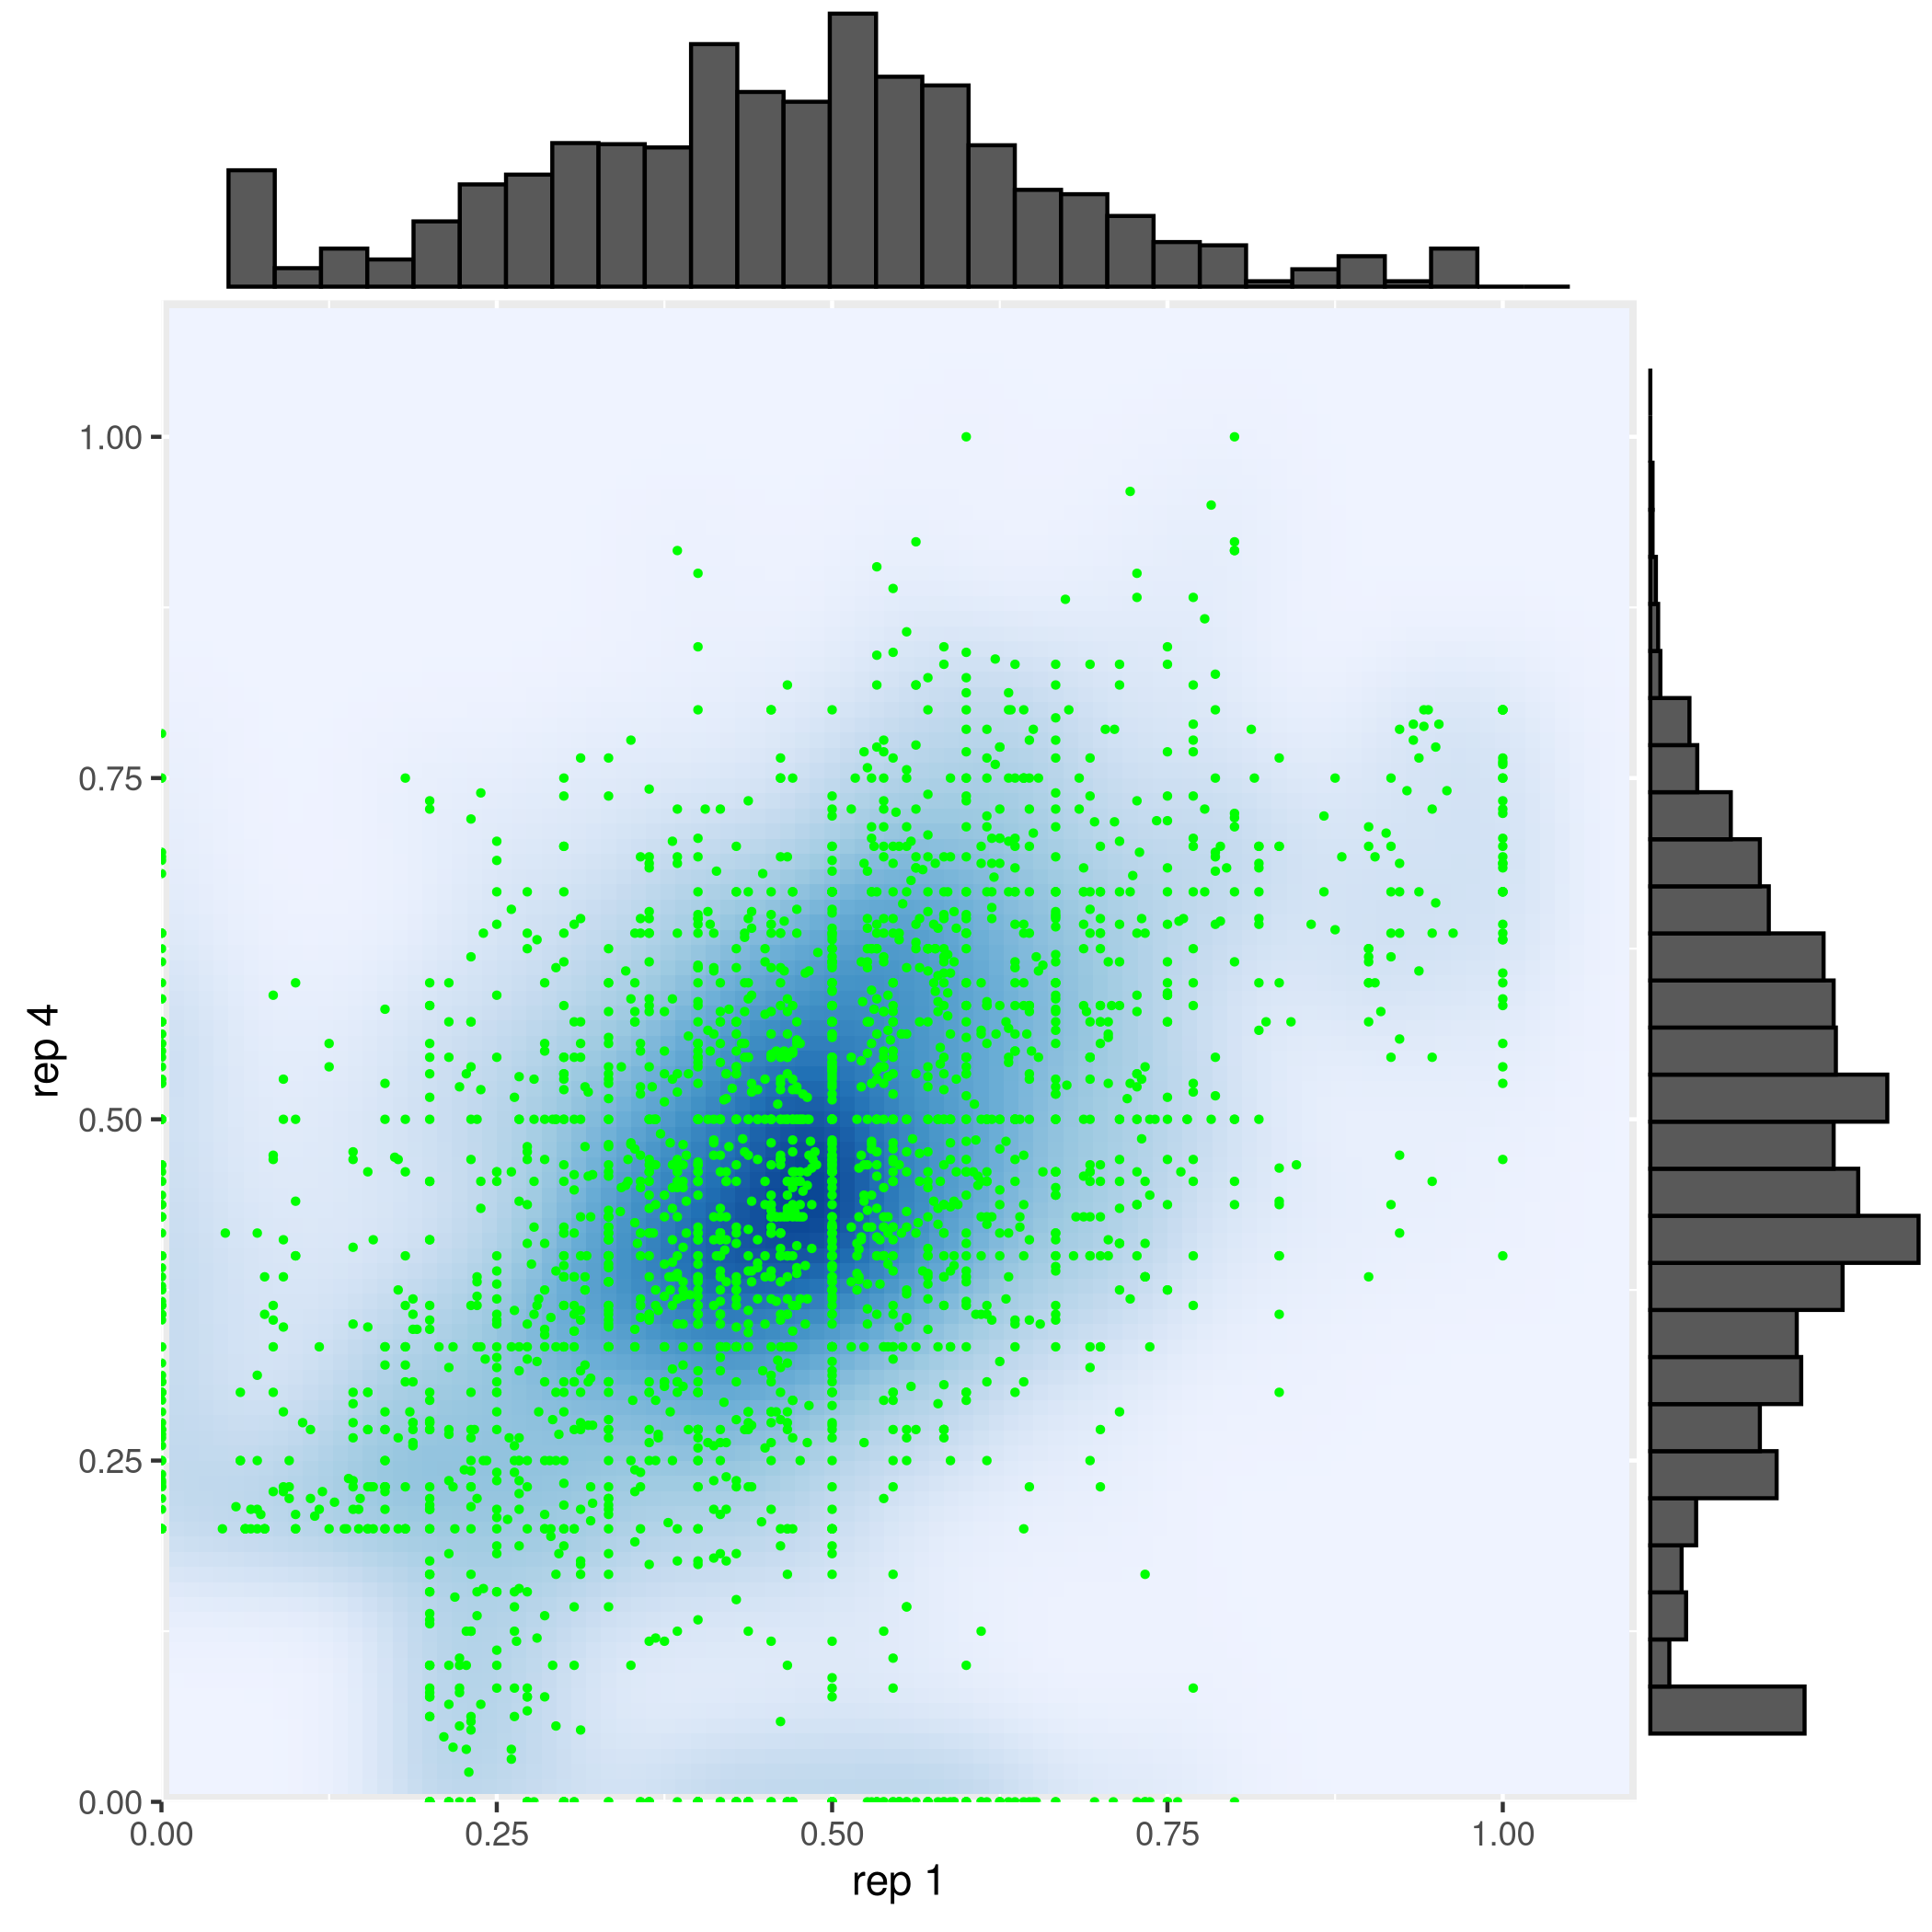
\includegraphics[width = 0.3\textwidth]{rep_corr/scr_DMSO_TOT-rep-1-4.post.0.2.0.8.10.png}} \\
      \subfloat[2 - 3]{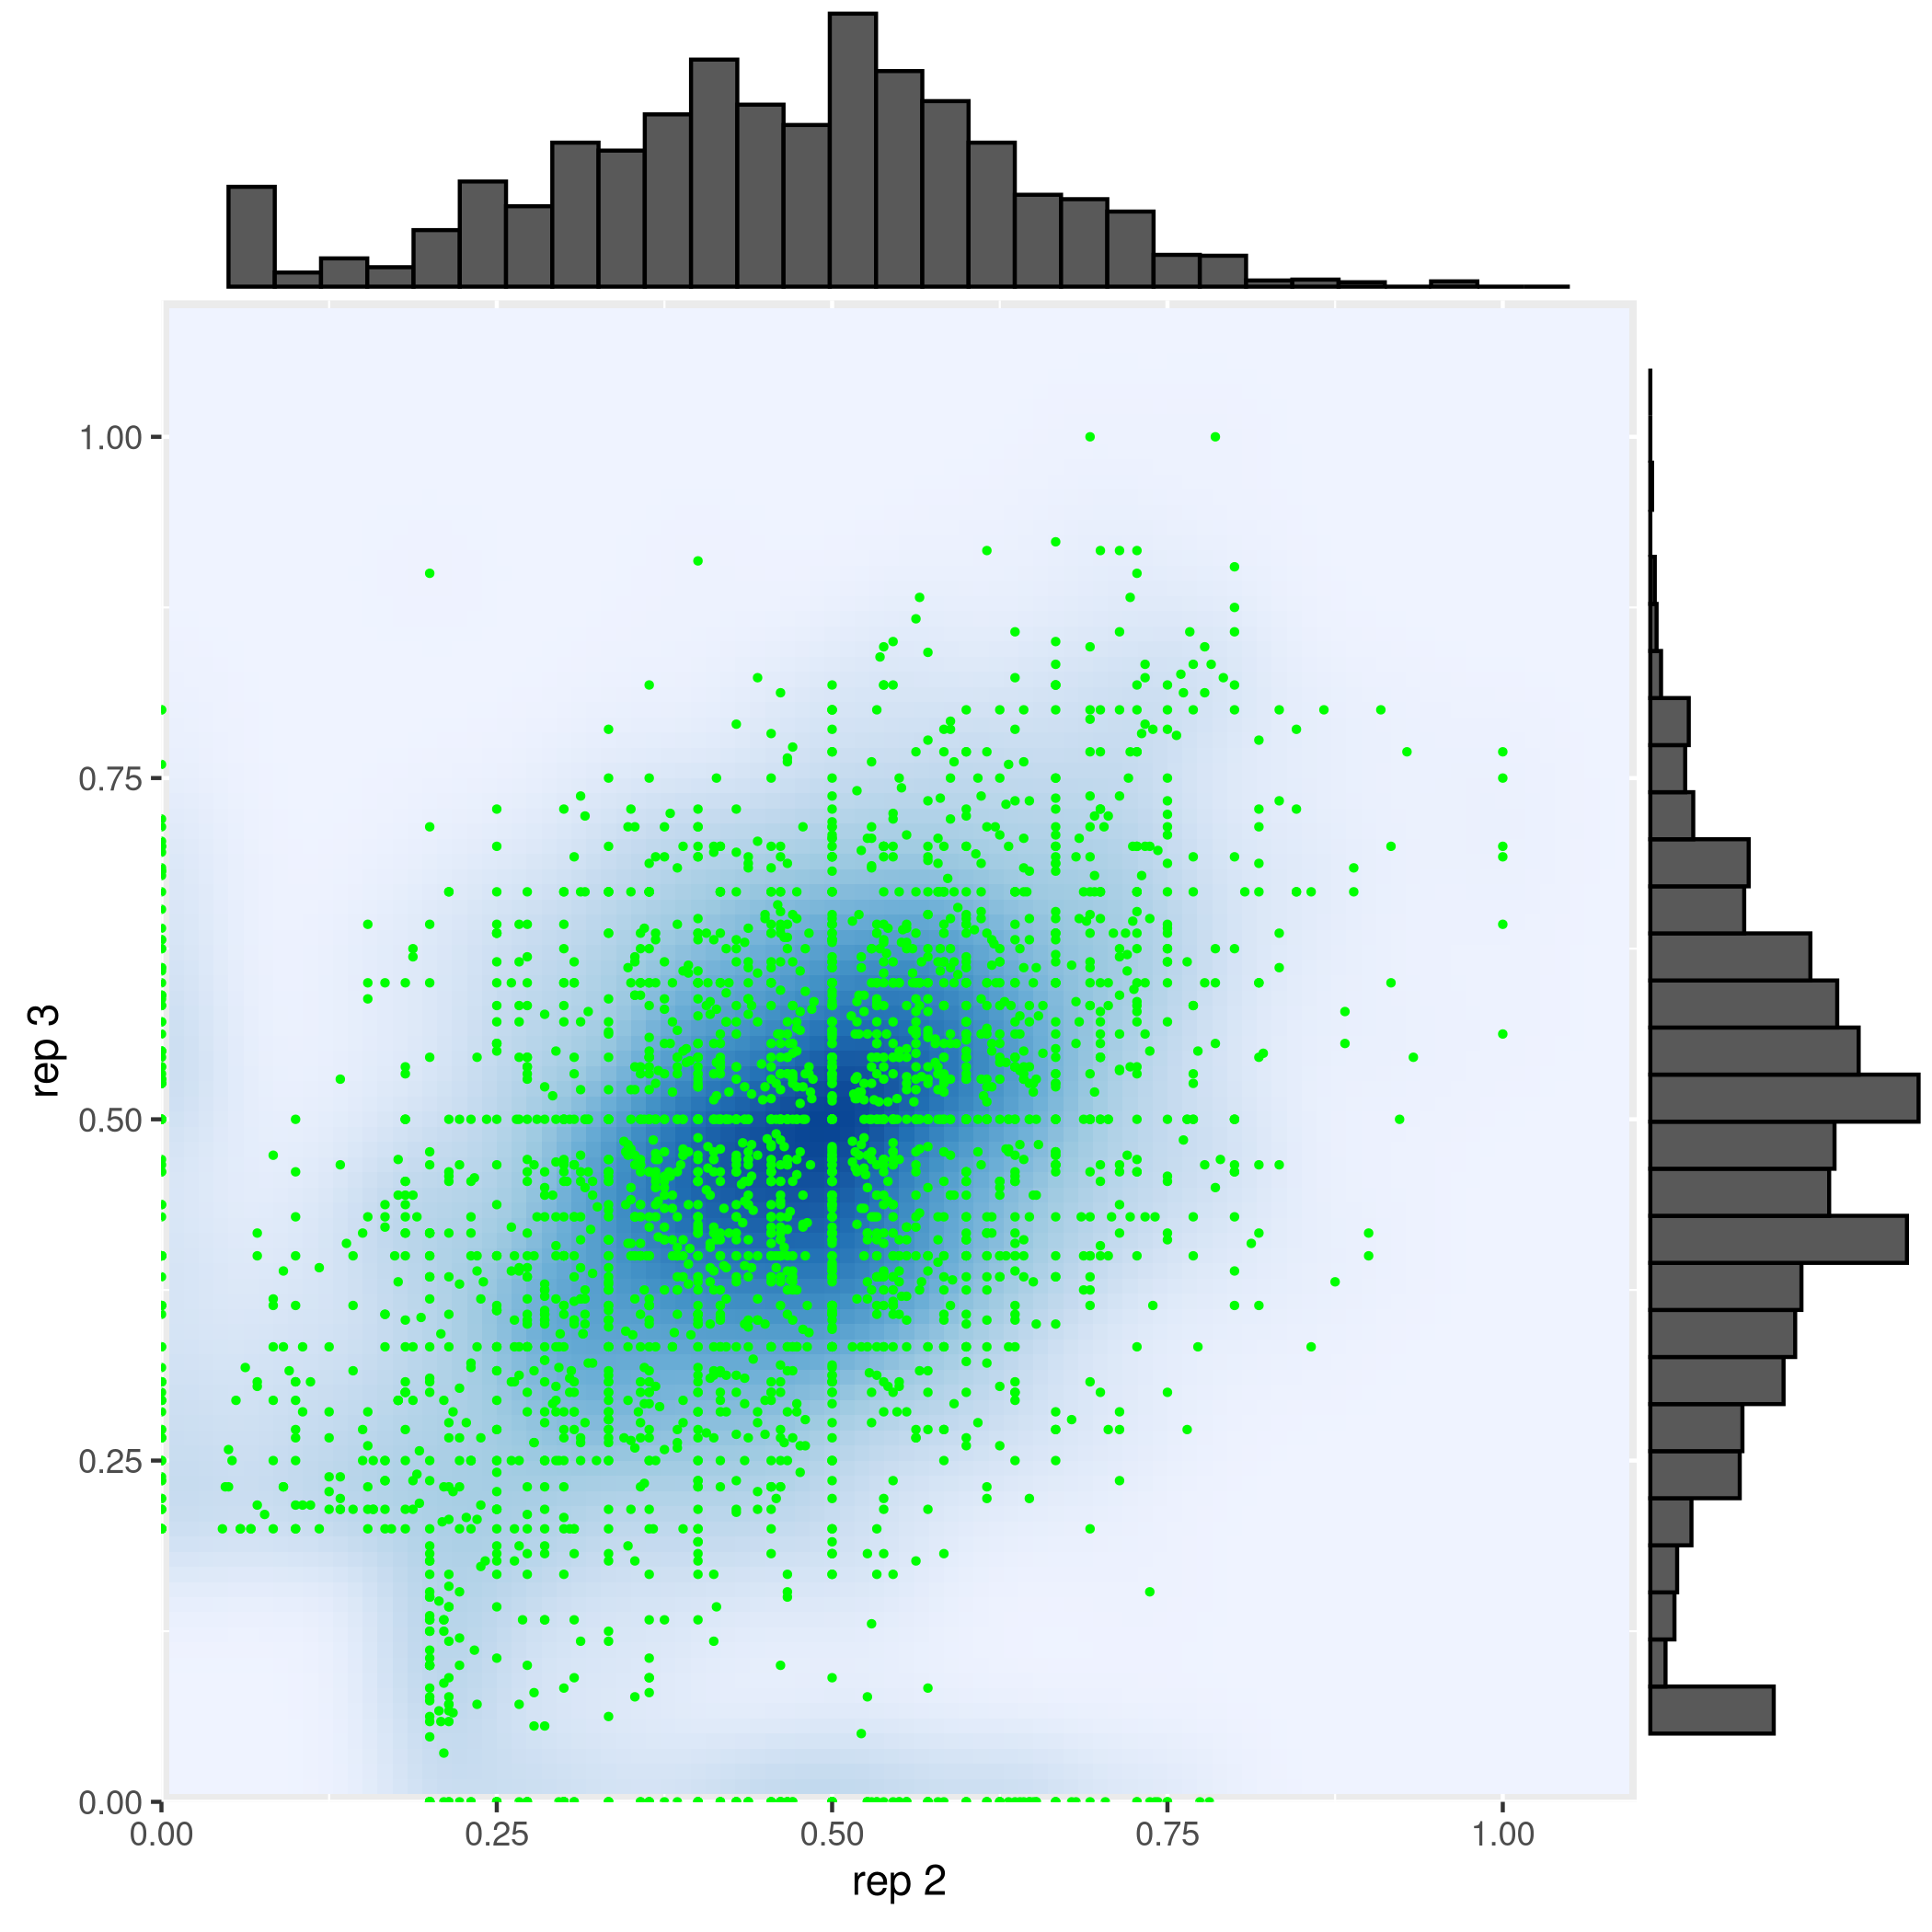
\includegraphics[width = 0.3\textwidth]{rep_corr/scr_DMSO_TOT-rep-2-3.post.0.2.0.8.10.png}} &
      \subfloat[2 - 4]{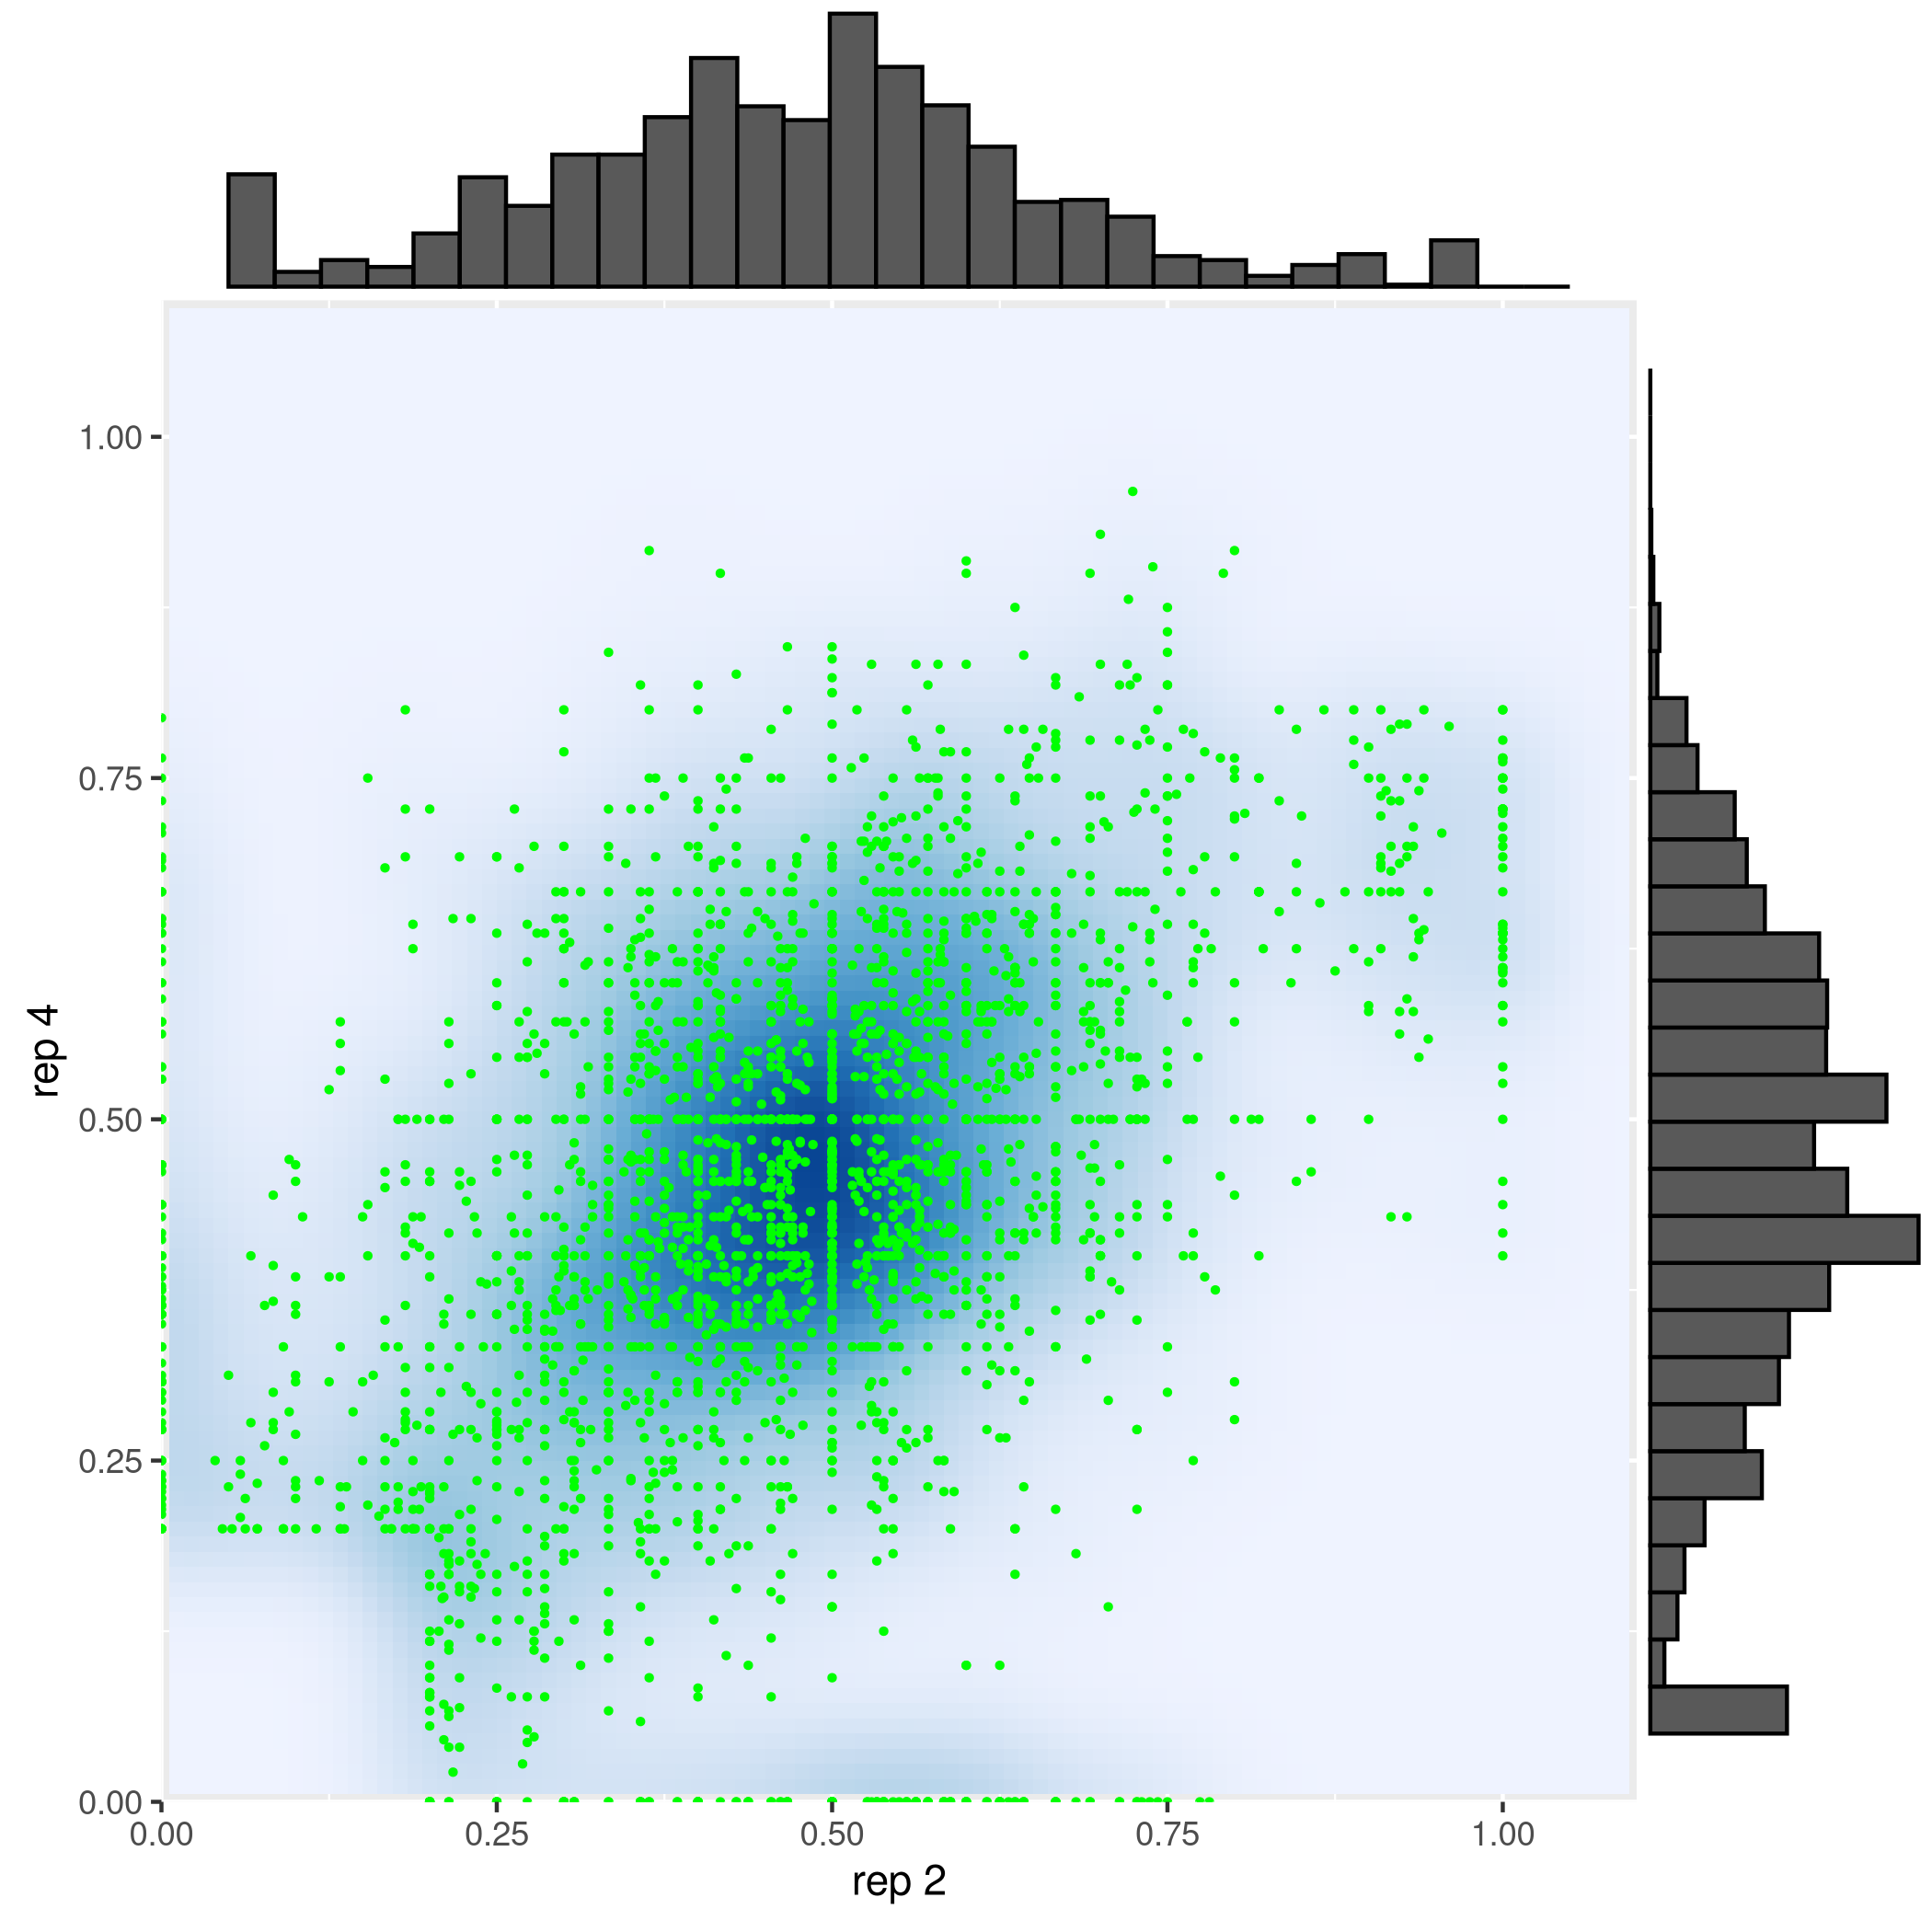
\includegraphics[width = 0.3\textwidth]{rep_corr/scr_DMSO_TOT-rep-2-4.post.0.2.0.8.10.png}} &
      \subfloat[3 - 4]{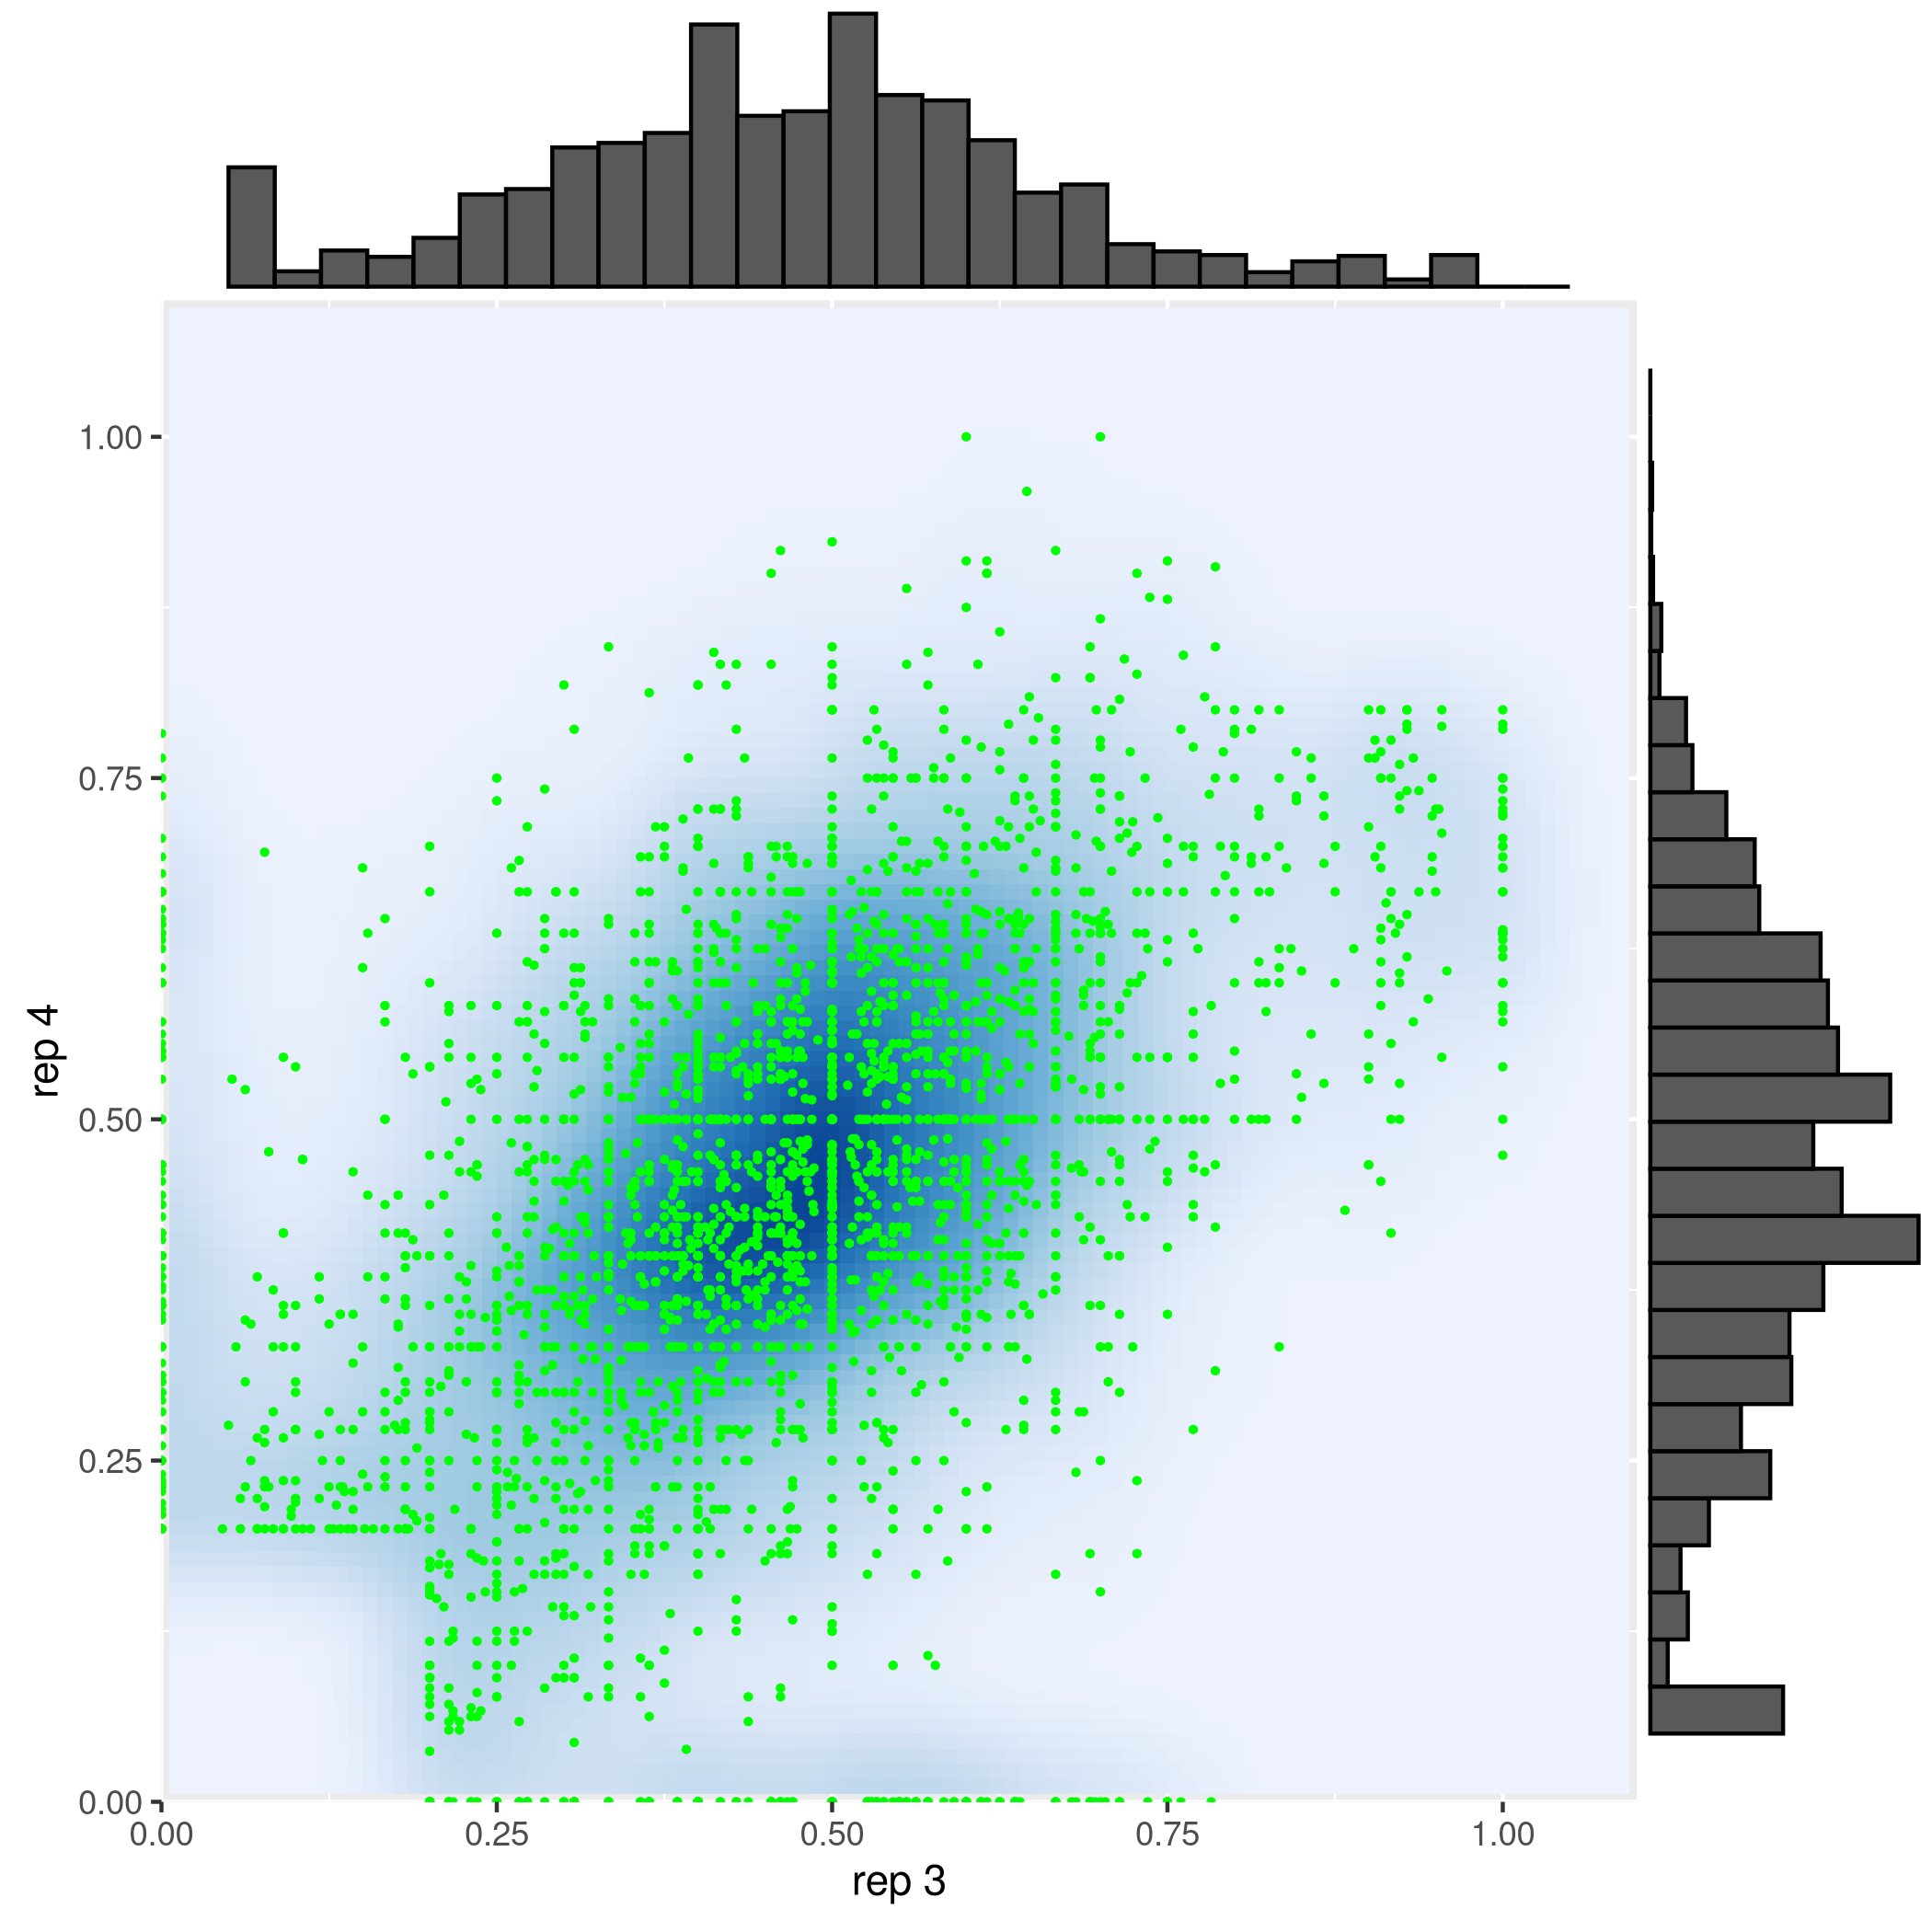
\includegraphics[width = 0.3\textwidth]{rep_corr/scr_DMSO_TOT-rep-3-4.post.0.2.0.8.10.png}} \\
  \end{tabular}
   \label{fig:}
 \end{figure}

\section{Considerazioni sulla recalibrazione}
\label{sec:rec_cons}
Discussione dei risultati di ASEQ prima e dopo la recalibrazione.
 \begin{figure}[H]
   \centering
   \begin{tabular}{ccc}
      \subfloat[scr DMSO polisomale]{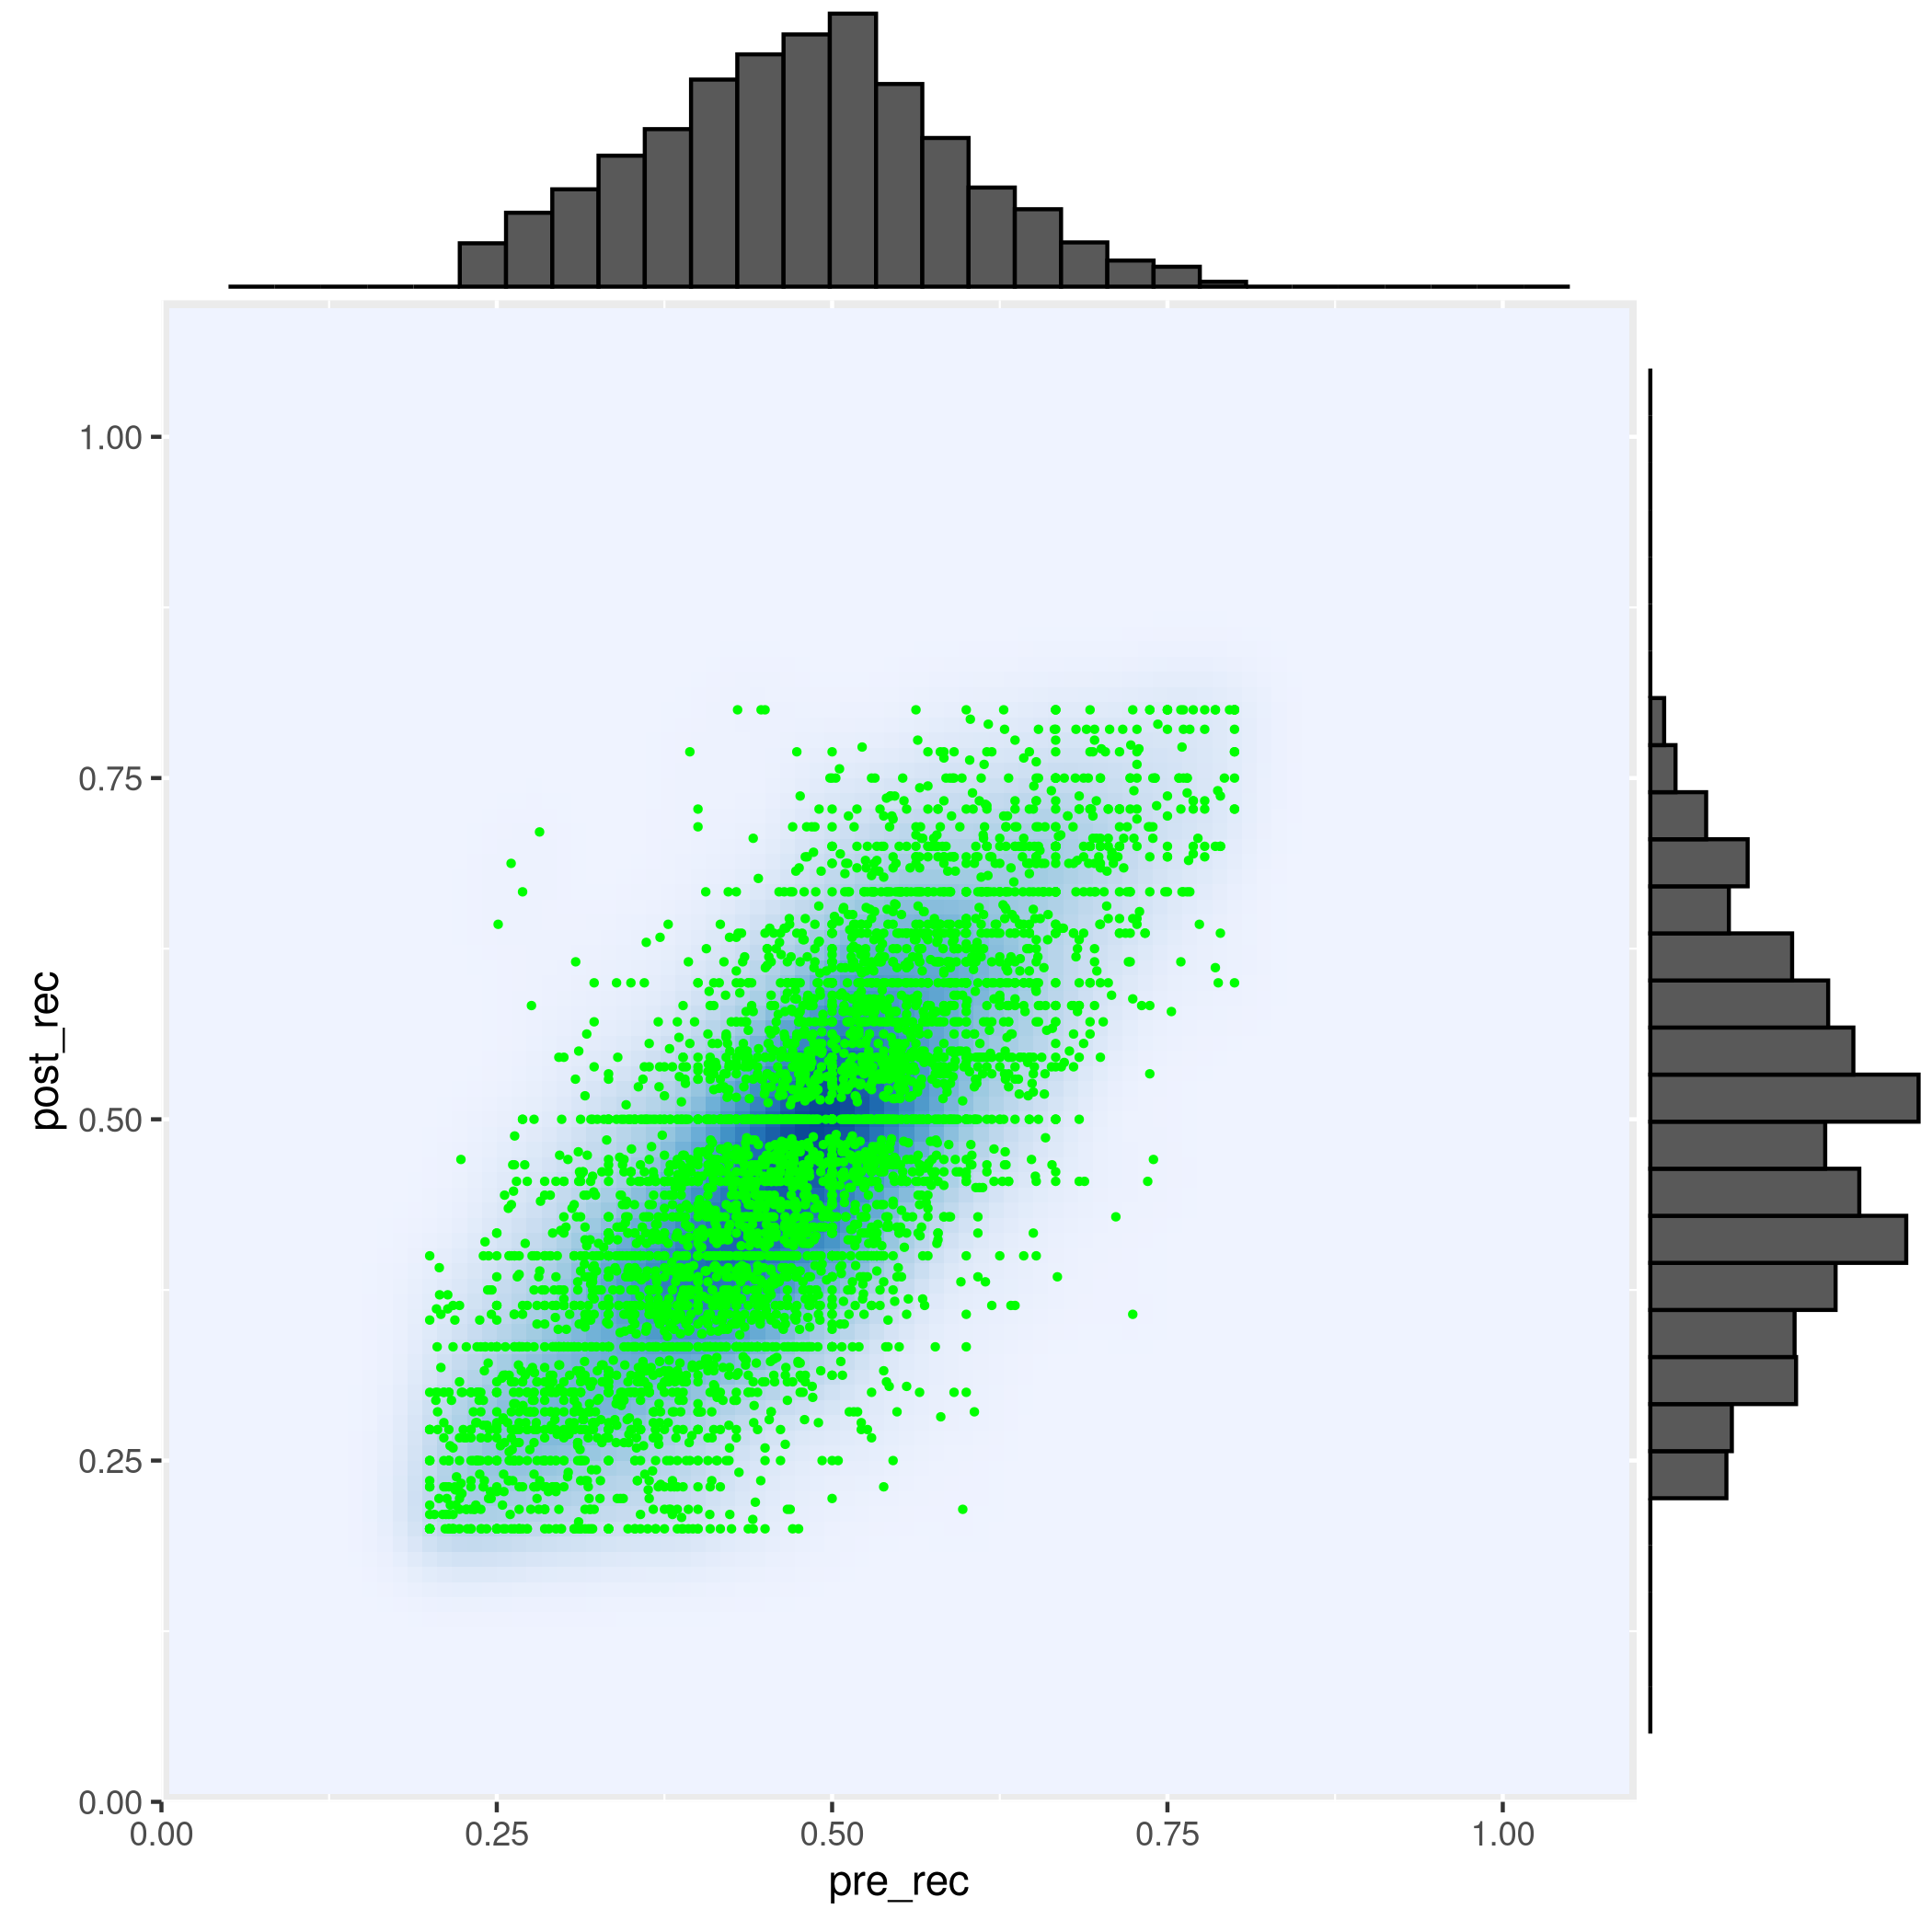
\includegraphics[width = 0.3\textwidth]{correlation_recal/scr_DMSO_POL_1.png}} &
      \subfloat[scr DMSO totale]{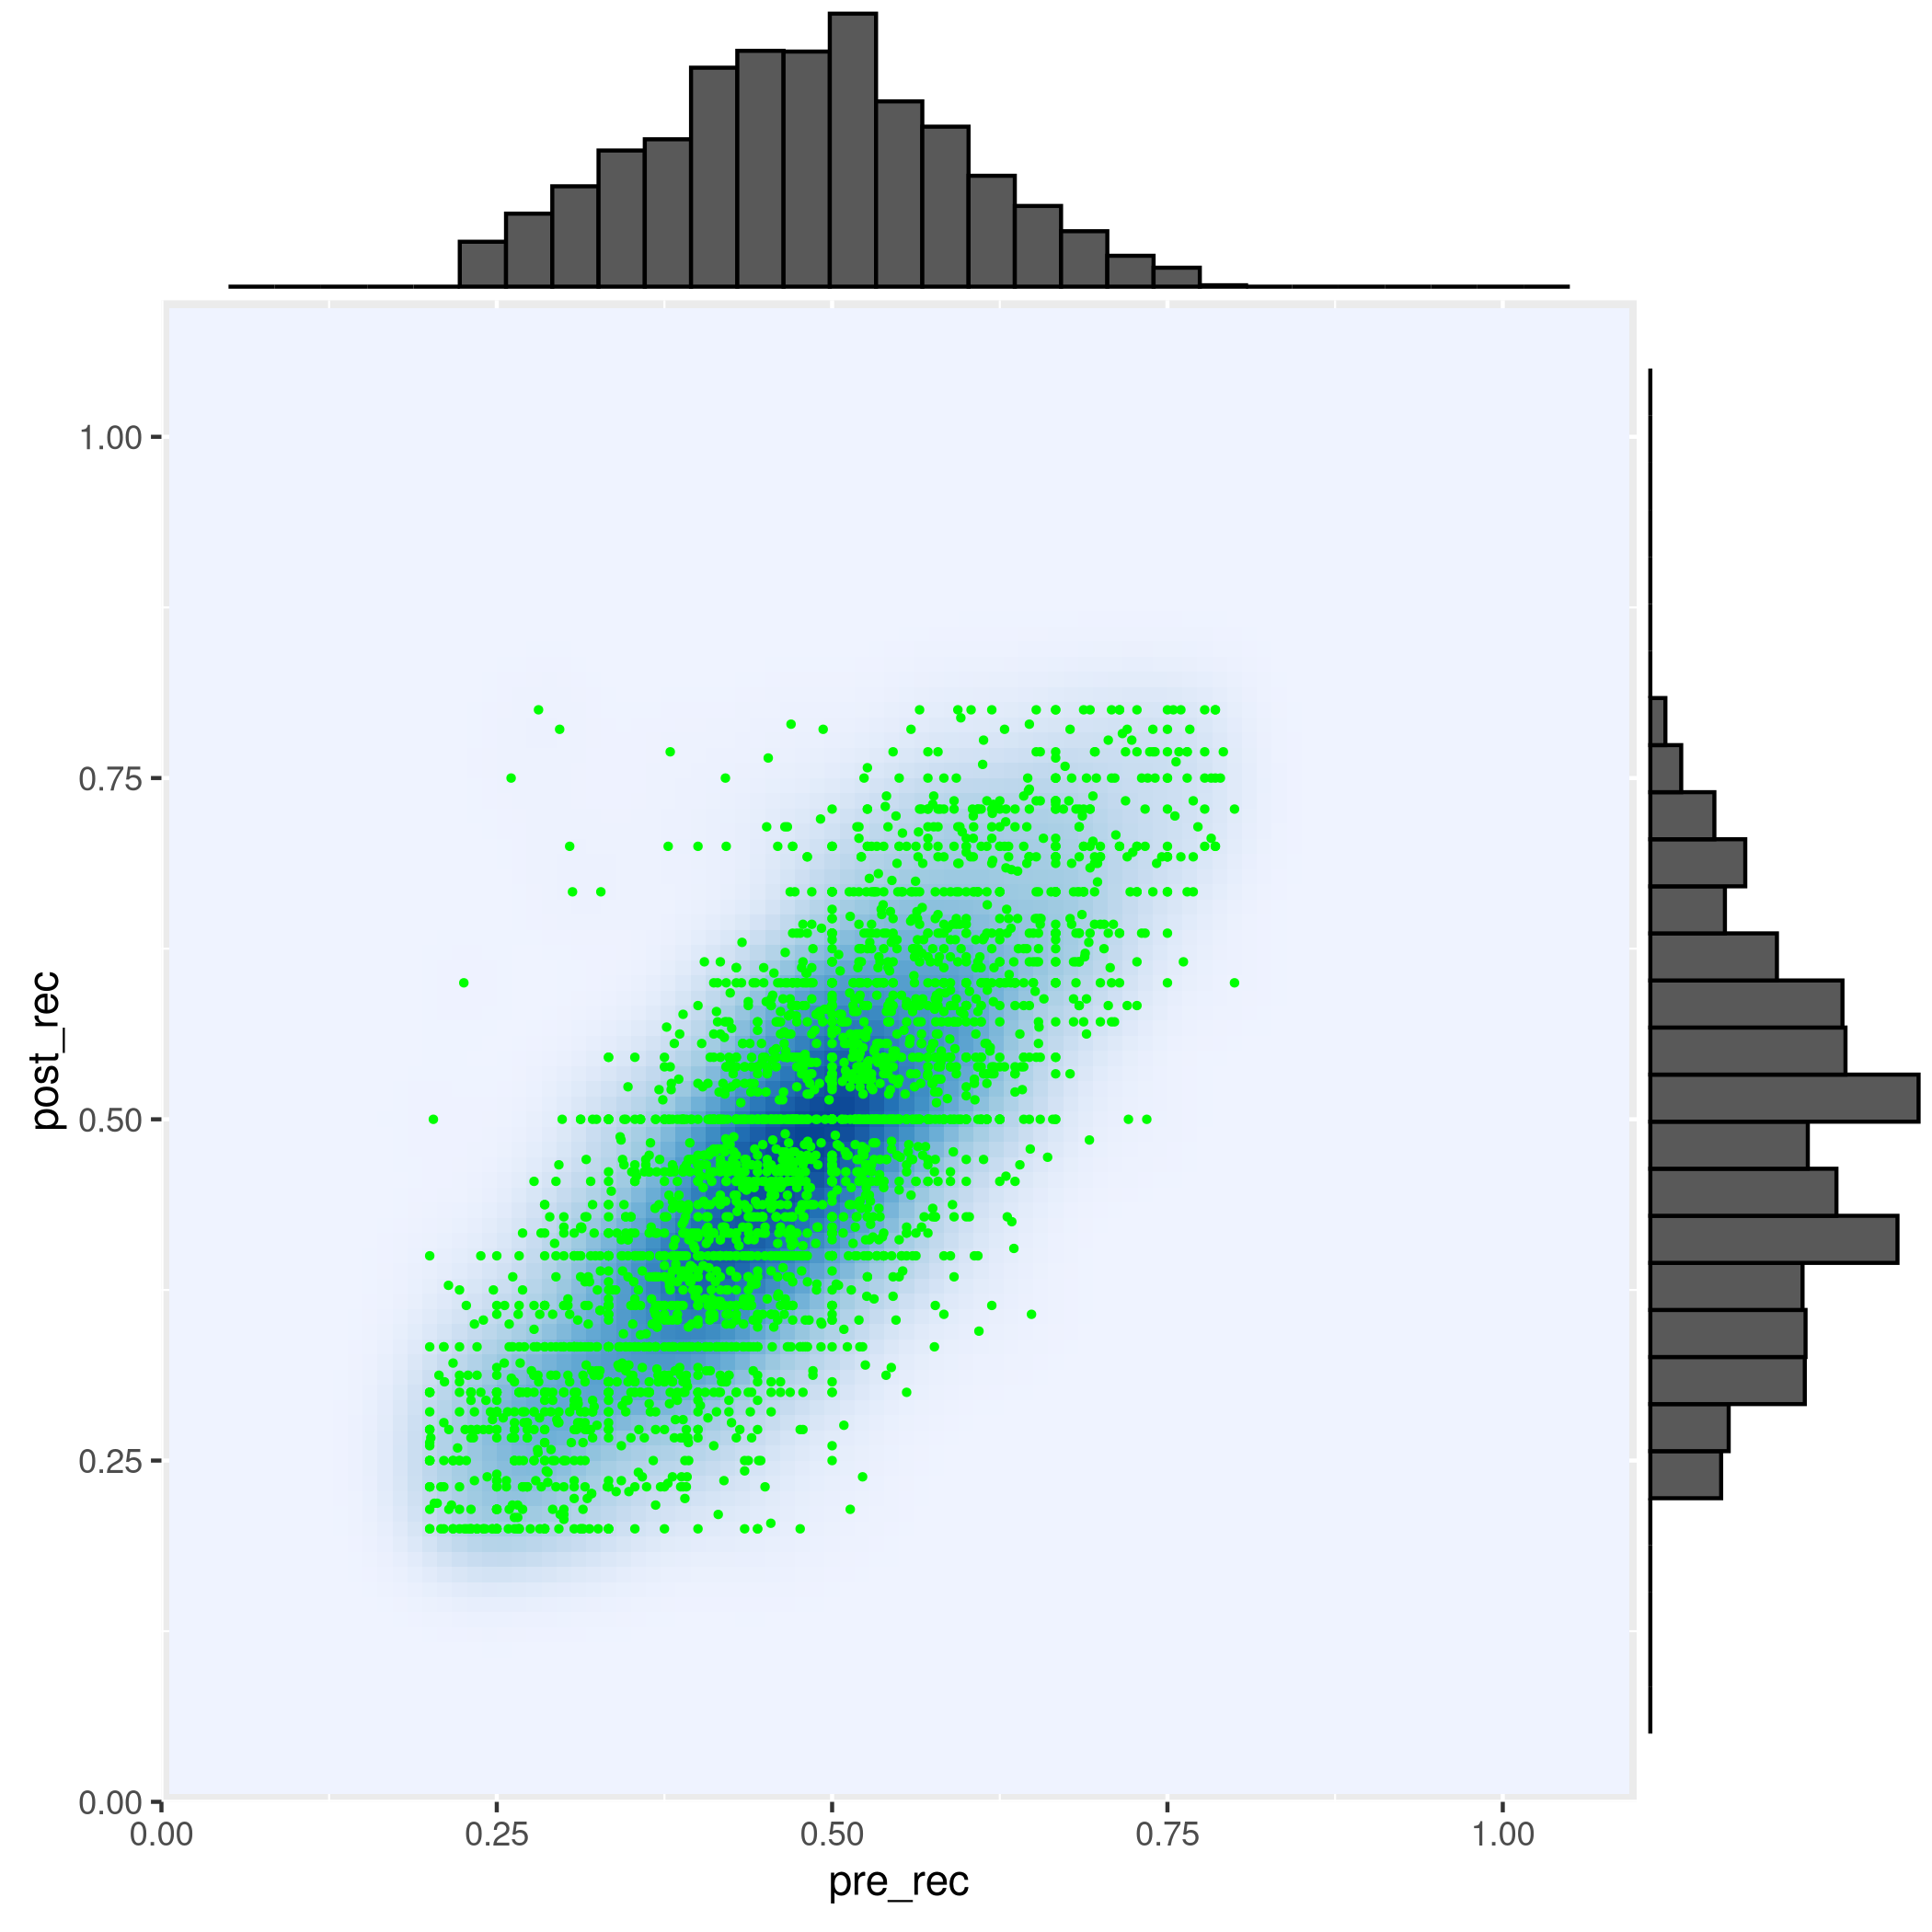
\includegraphics[width = 0.3\textwidth]{correlation_recal/scr_DMSO_TOT_1.png}} &
      \subfloat[scr NUTLIN polisomale]{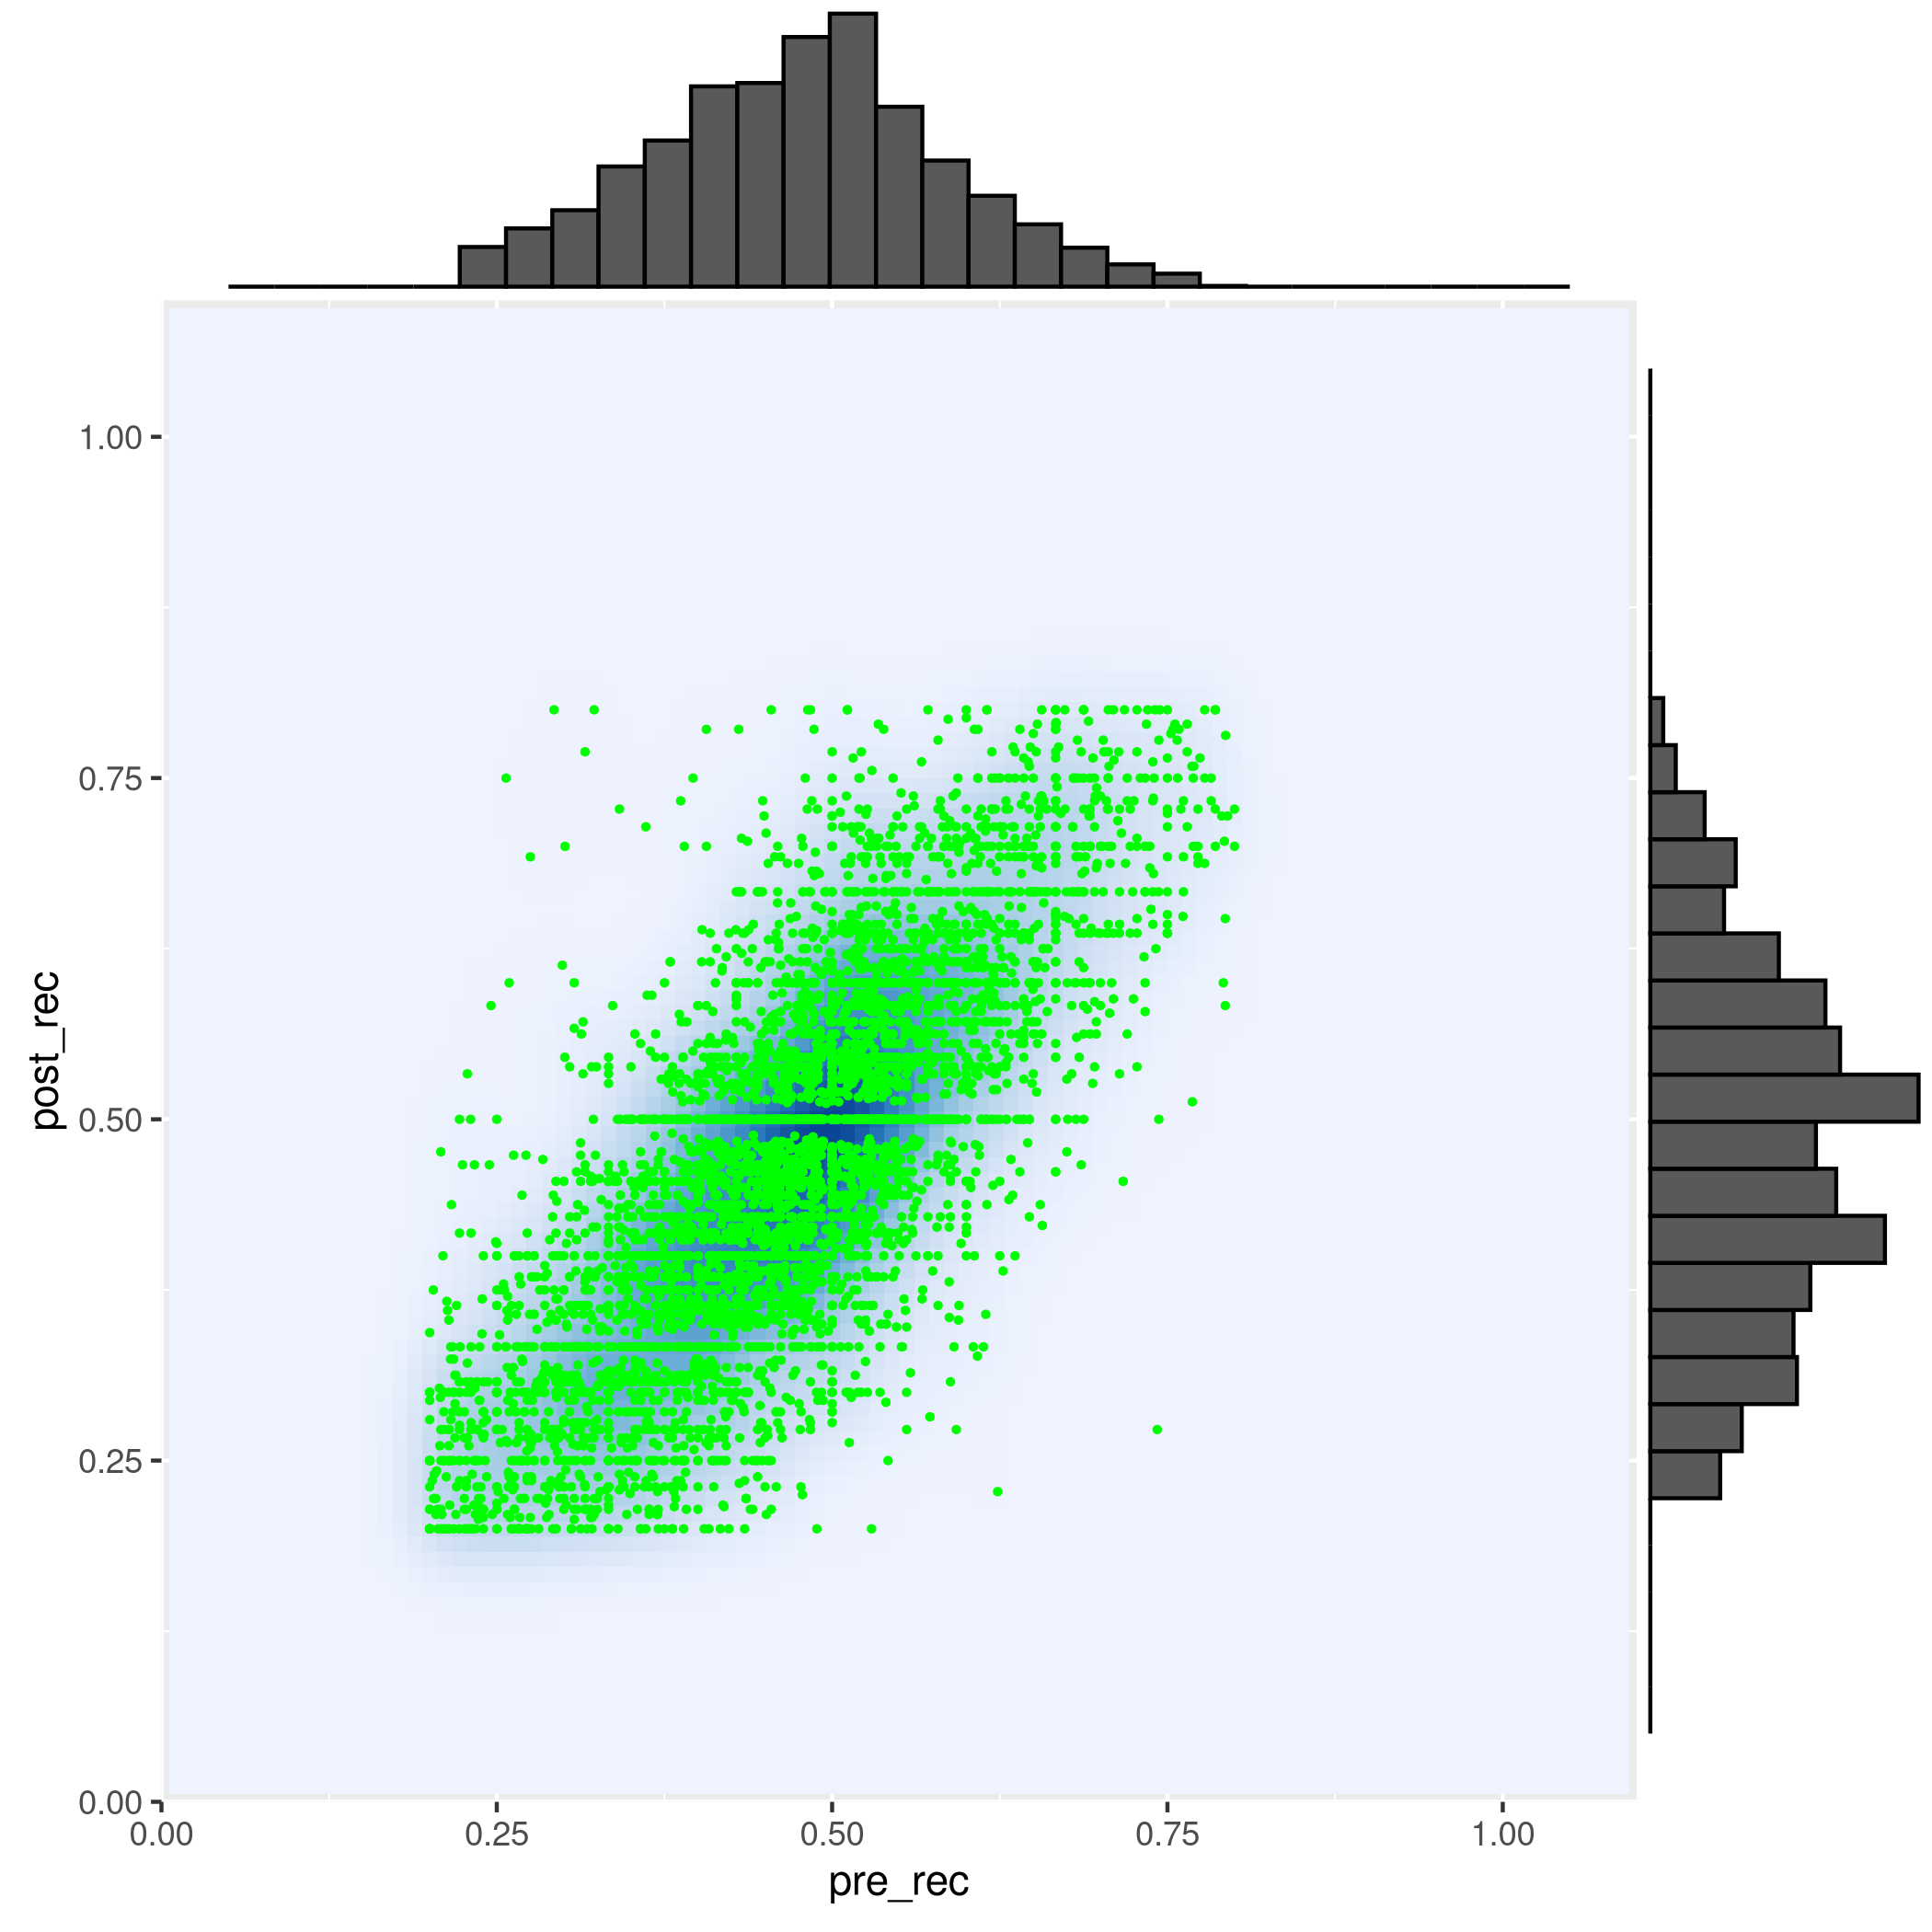
\includegraphics[width = 0.3\textwidth]{correlation_recal/scr_NUTLIN_POL_1.png}} \\
      \subfloat[scr NUTLIN totale]{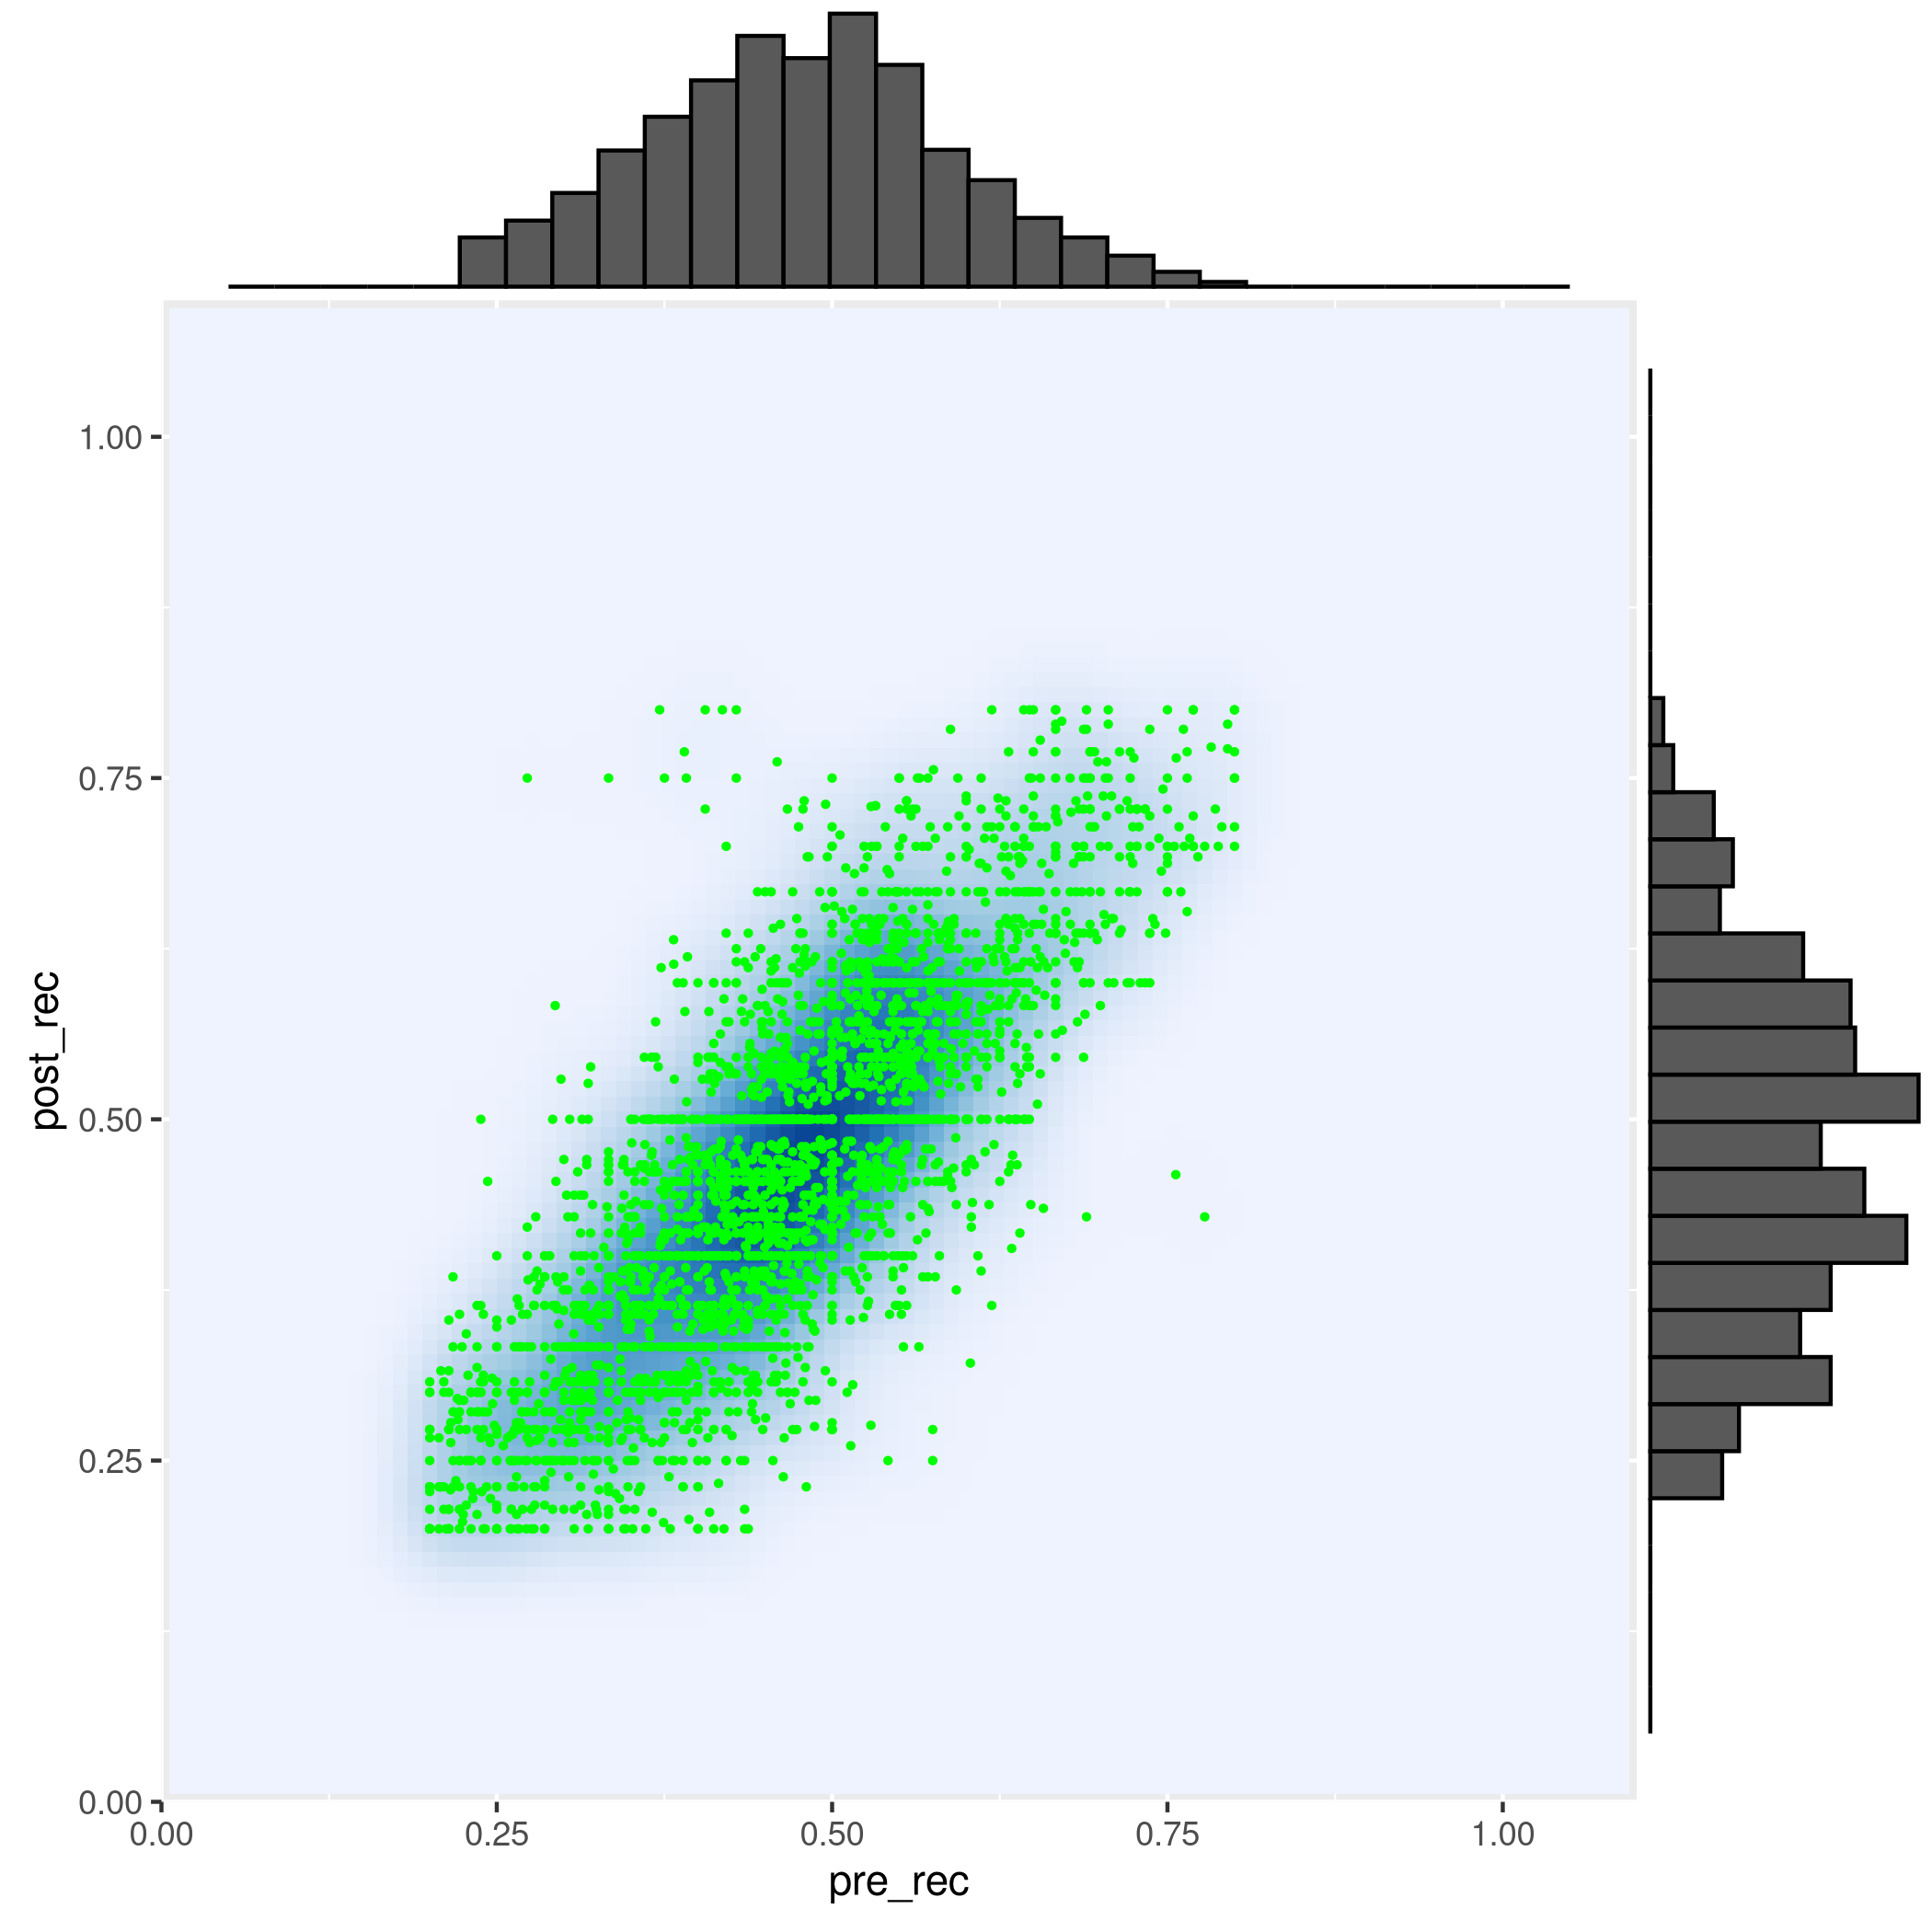
\includegraphics[width = 0.3\textwidth]{correlation_recal/scr_NUTLIN_TOT_1.png}} &
      \subfloat[shDHX30 DMSO polisomale]{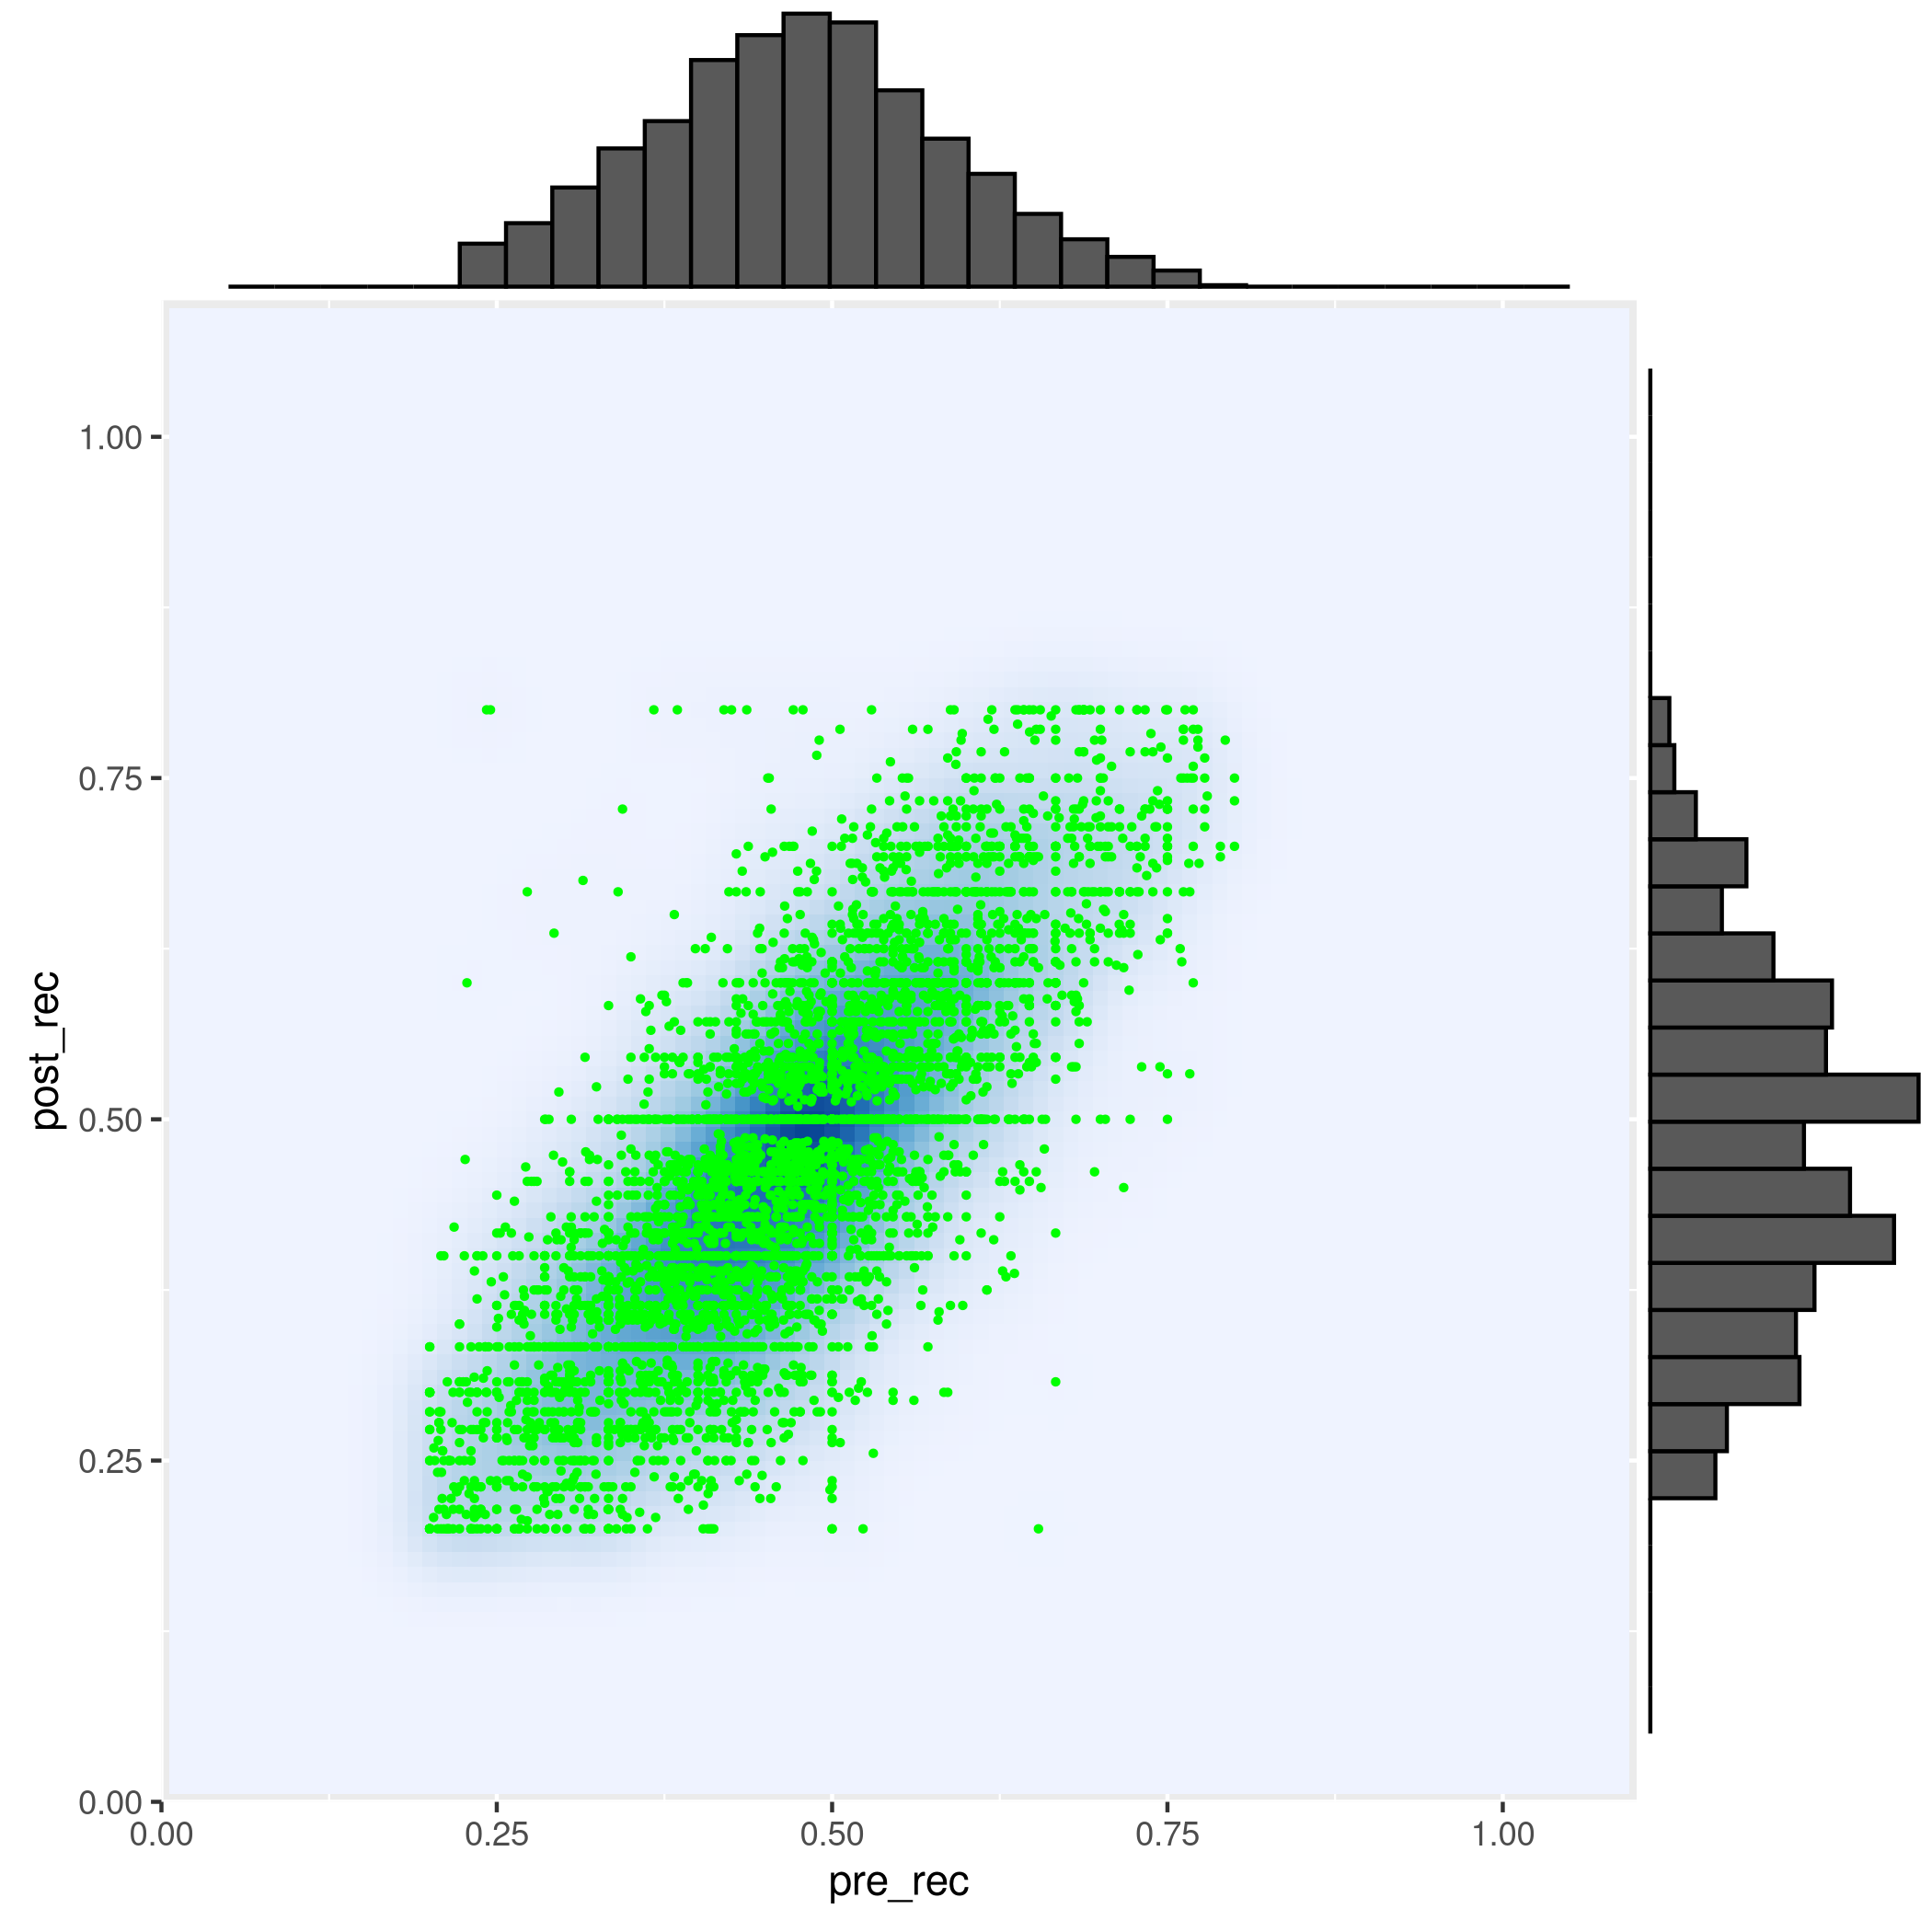
\includegraphics[width = 0.3\textwidth]{correlation_recal/shDHX30_DMSO_POL_1.png}} &
      \subfloat[shDHX30 DMSO totale]{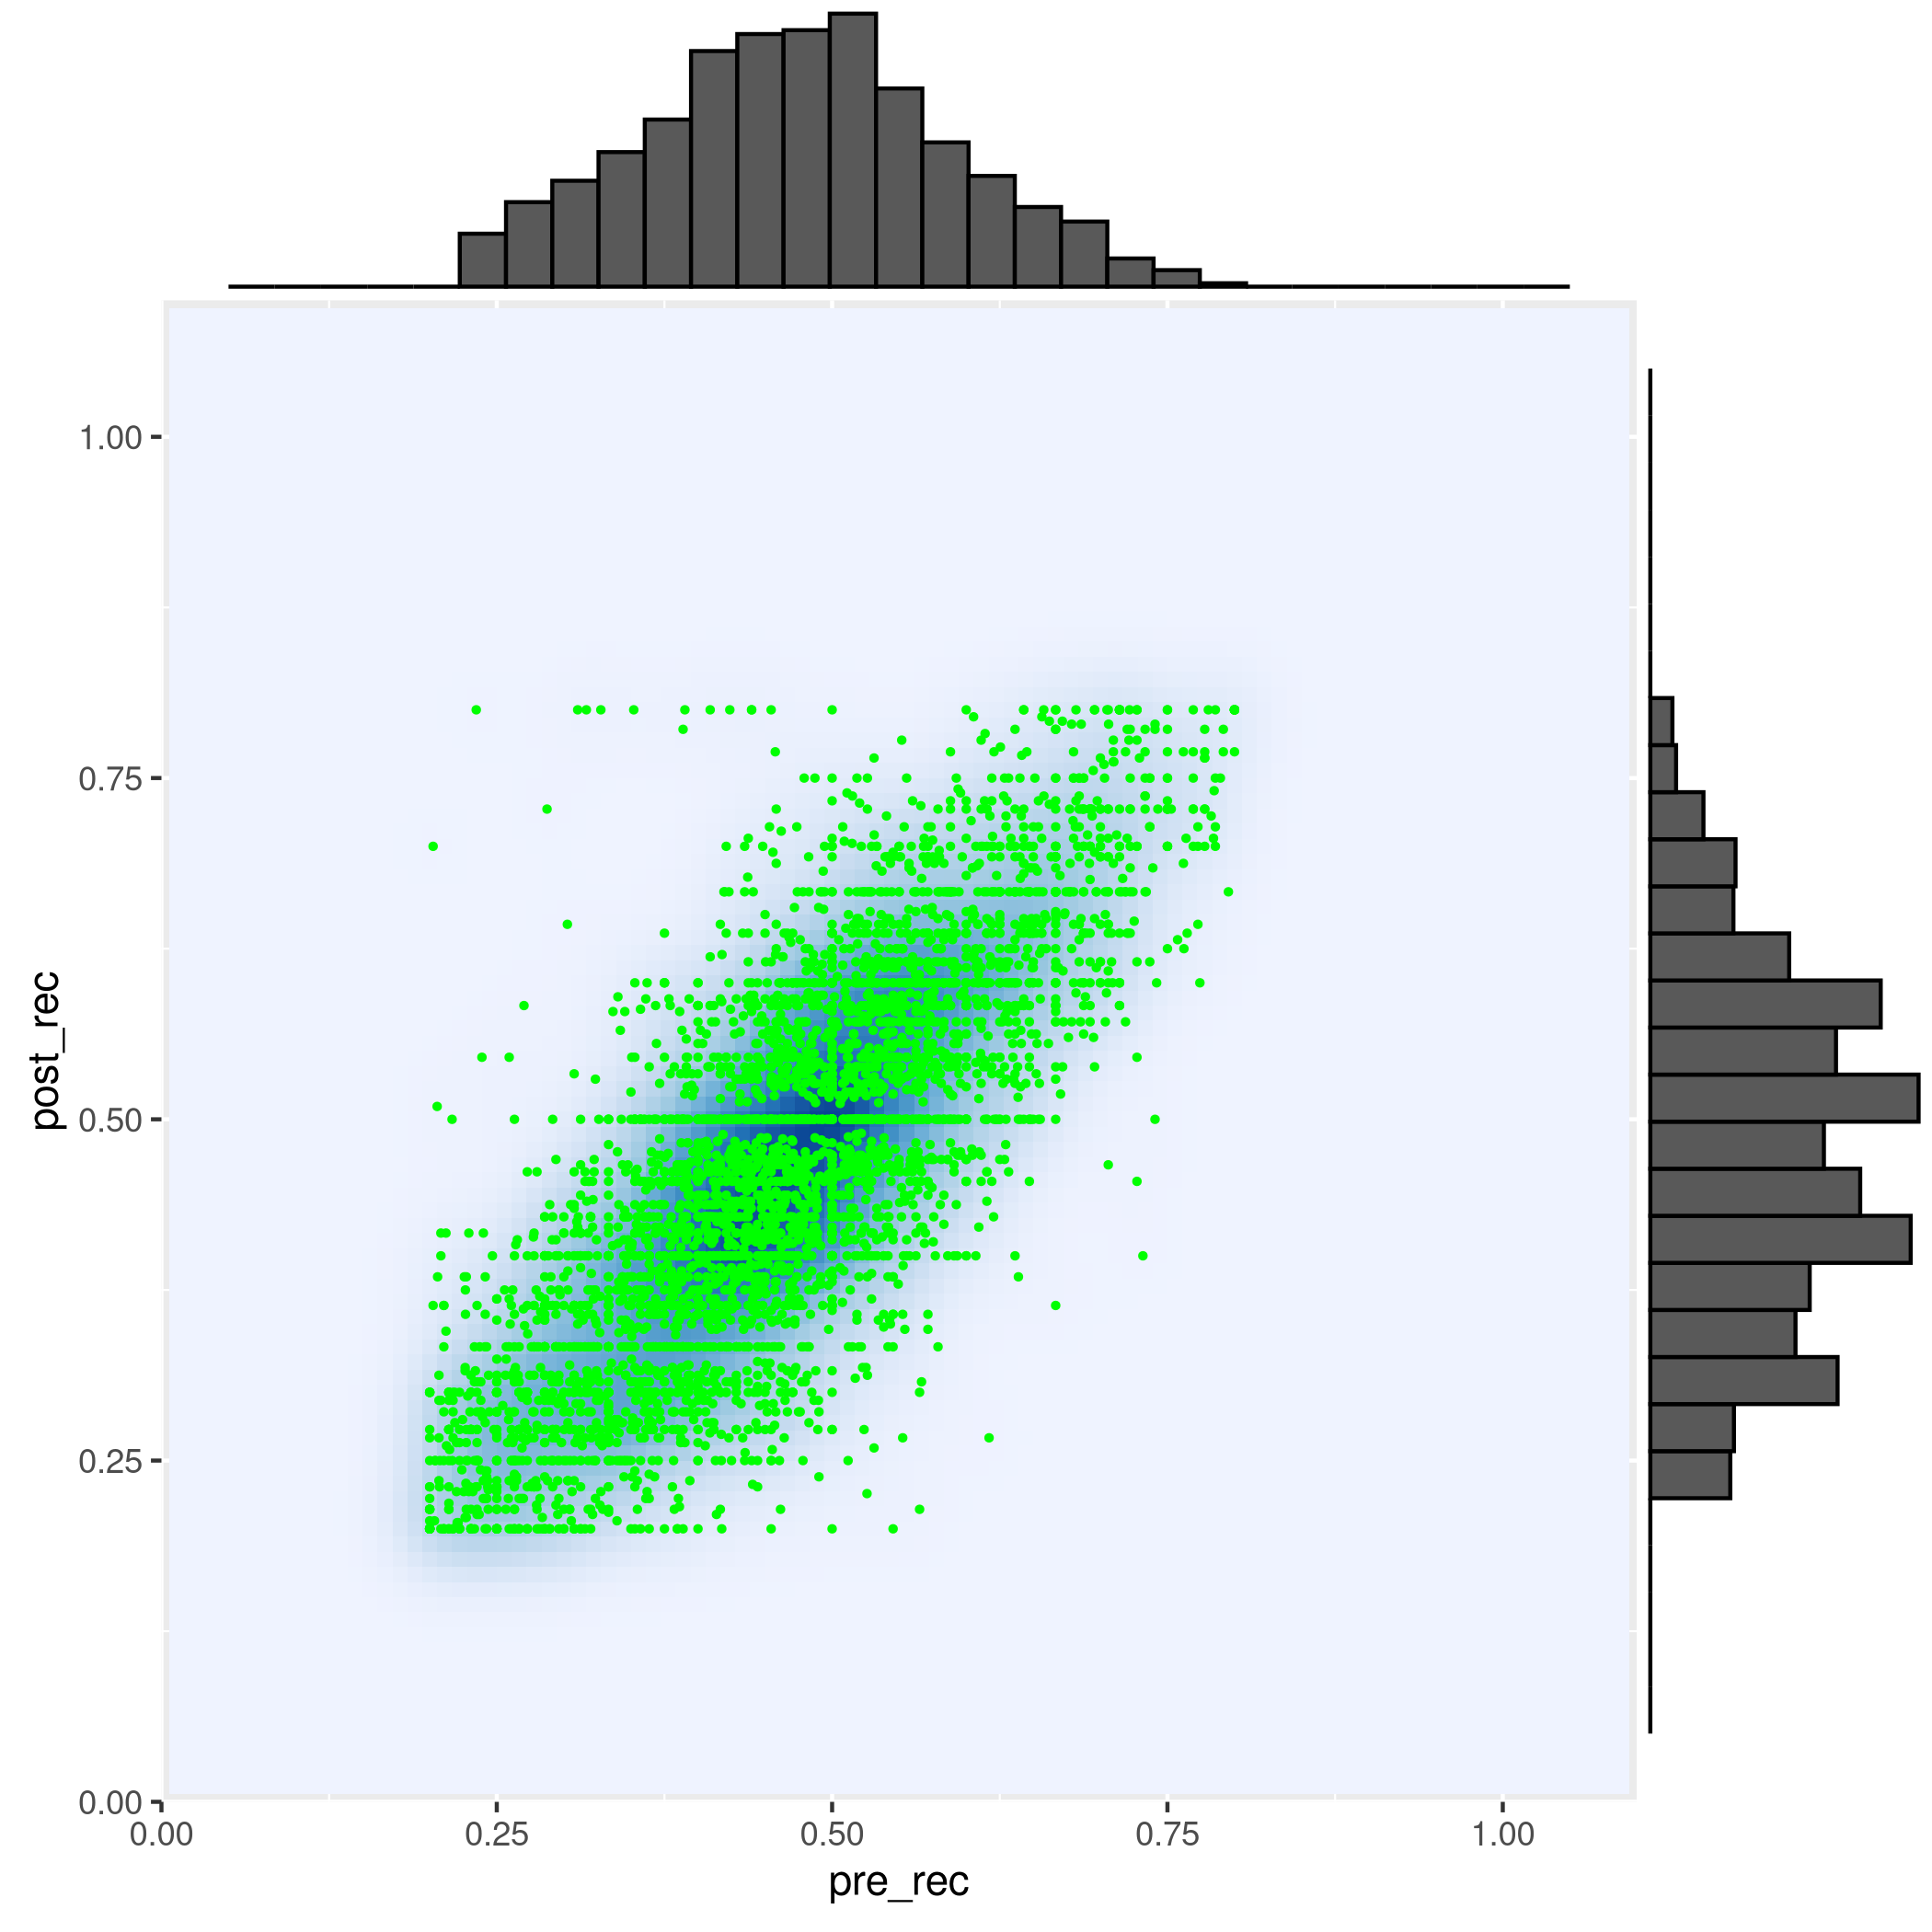
\includegraphics[width = 0.3\textwidth]{correlation_recal/shDHX30_DMSO_TOT_1.png}} \\
      \subfloat[shDHX30 NUTLIN polisomale]{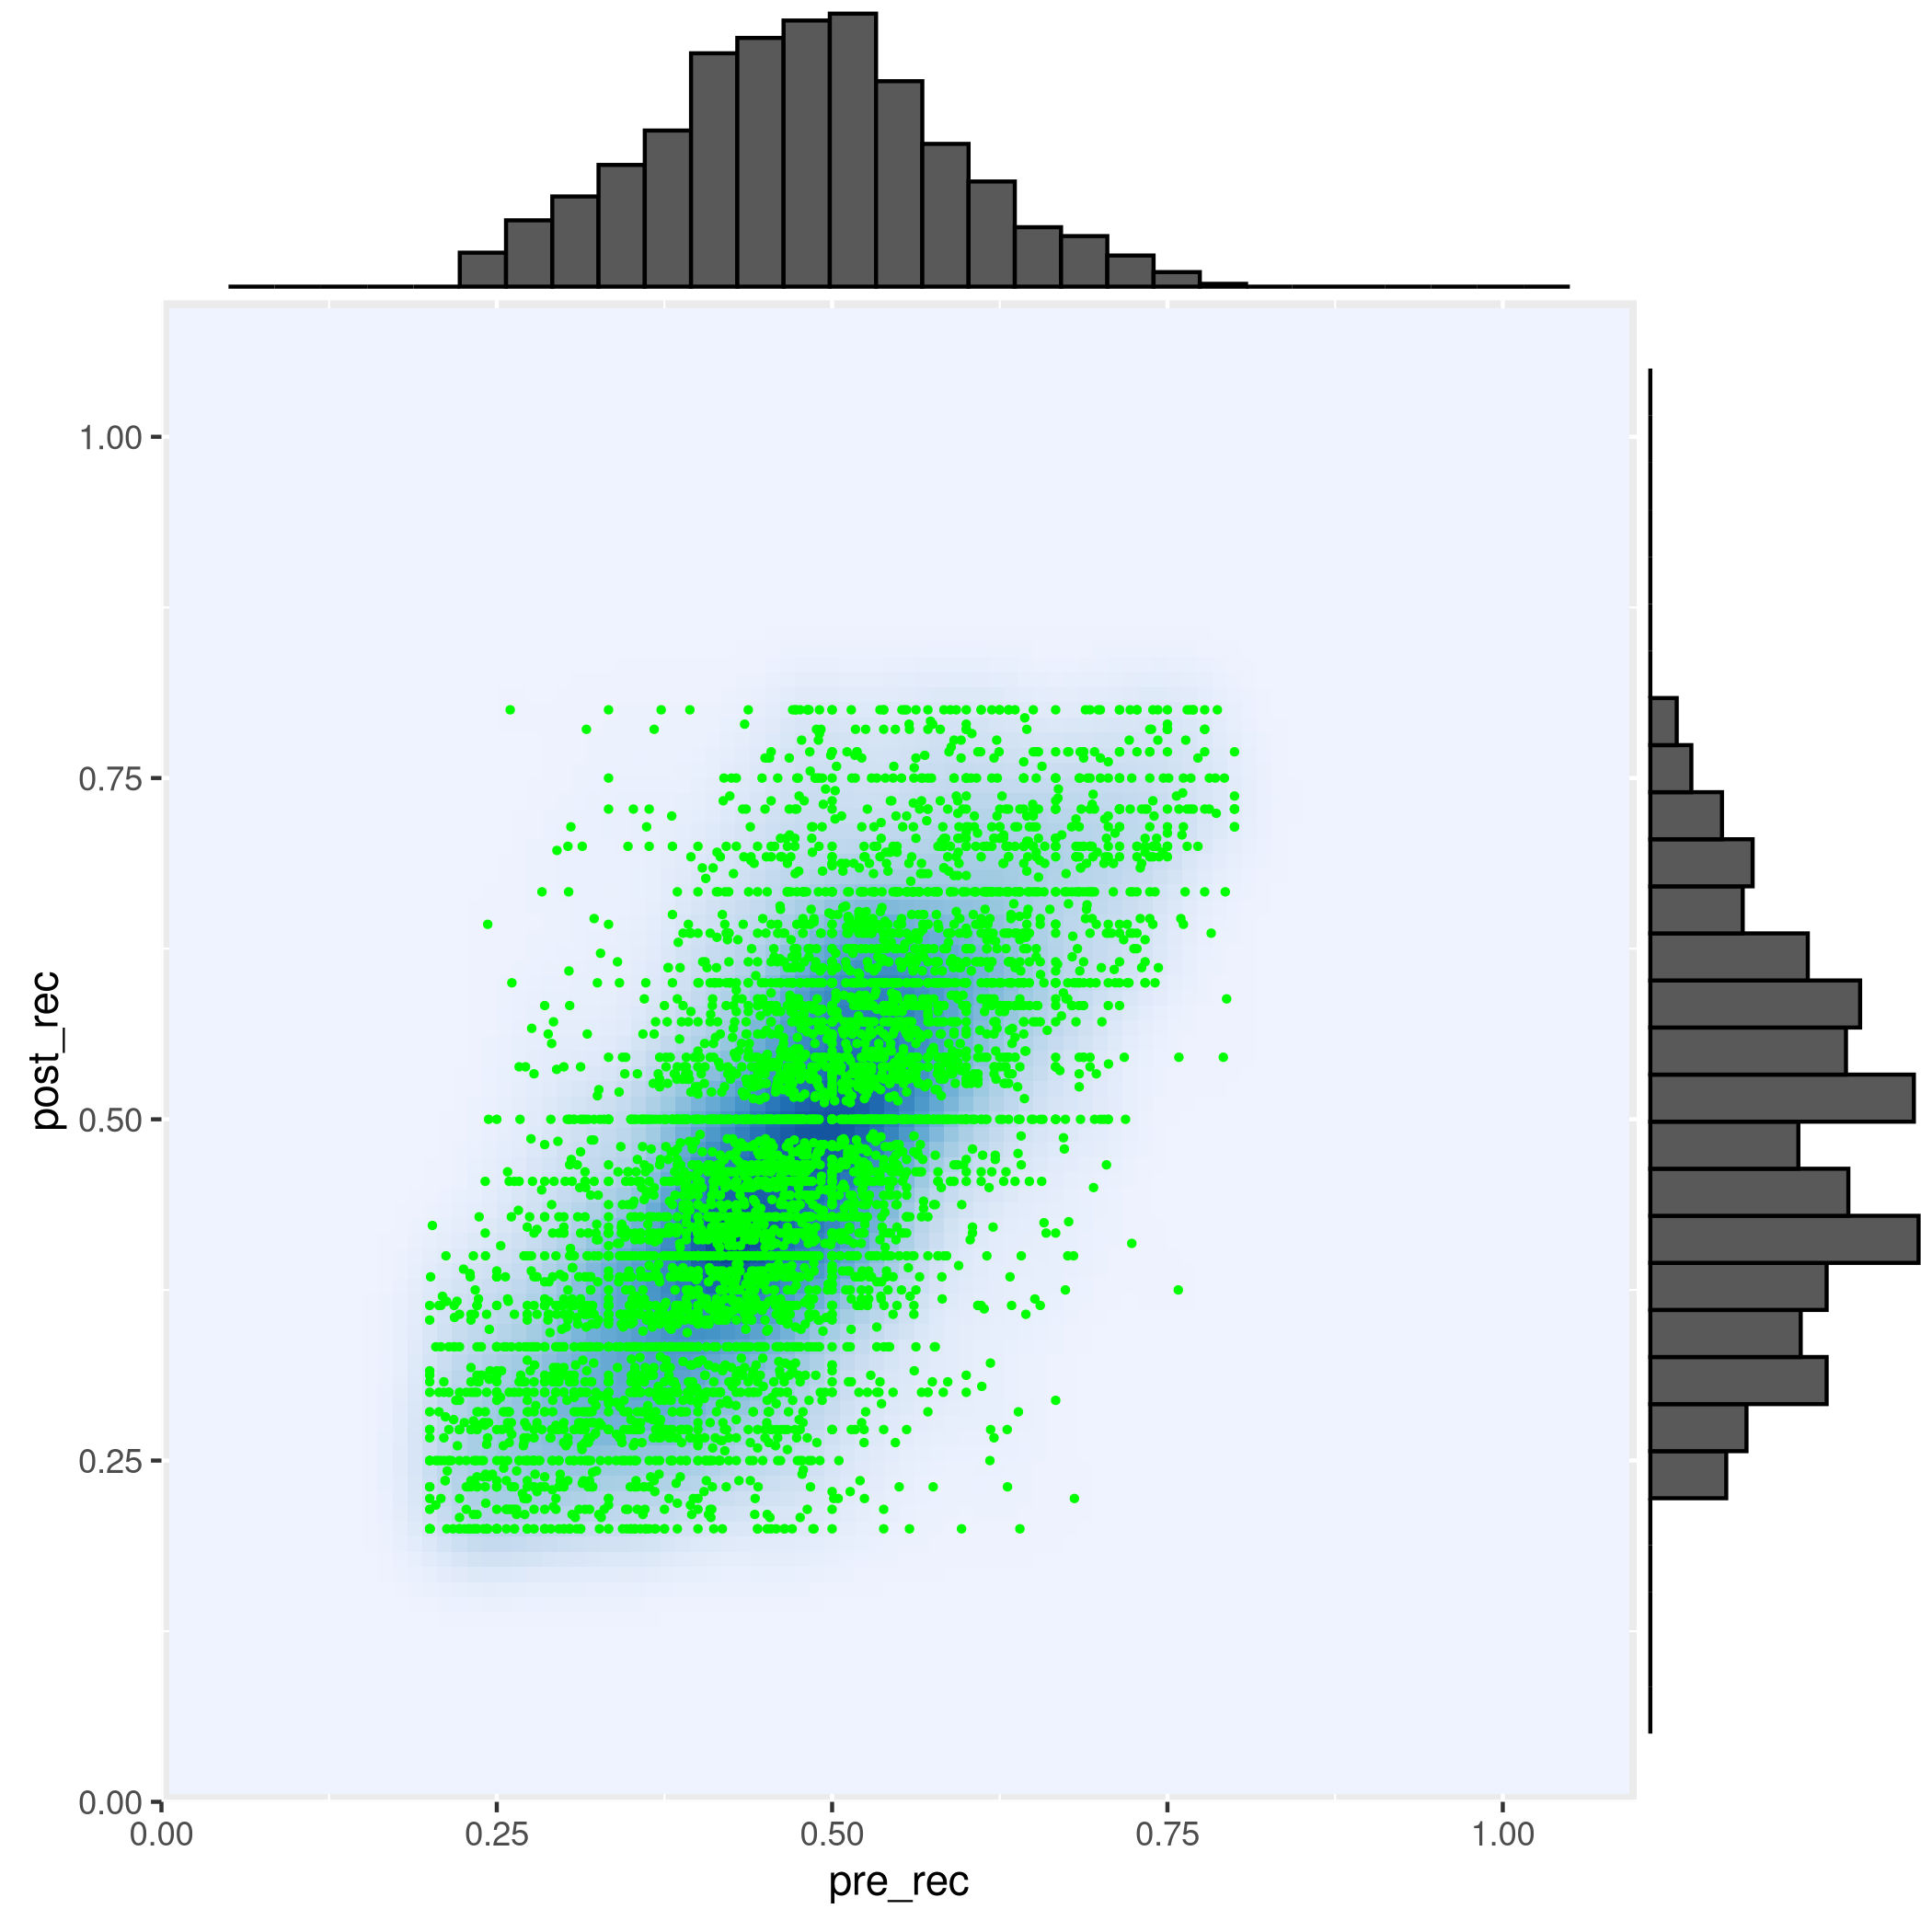
\includegraphics[width = 0.3\textwidth]{correlation_recal/shDHX30_NUTLIN_POL_1.png}} &
      \subfloat[shDHX30 NUTLIN totale]{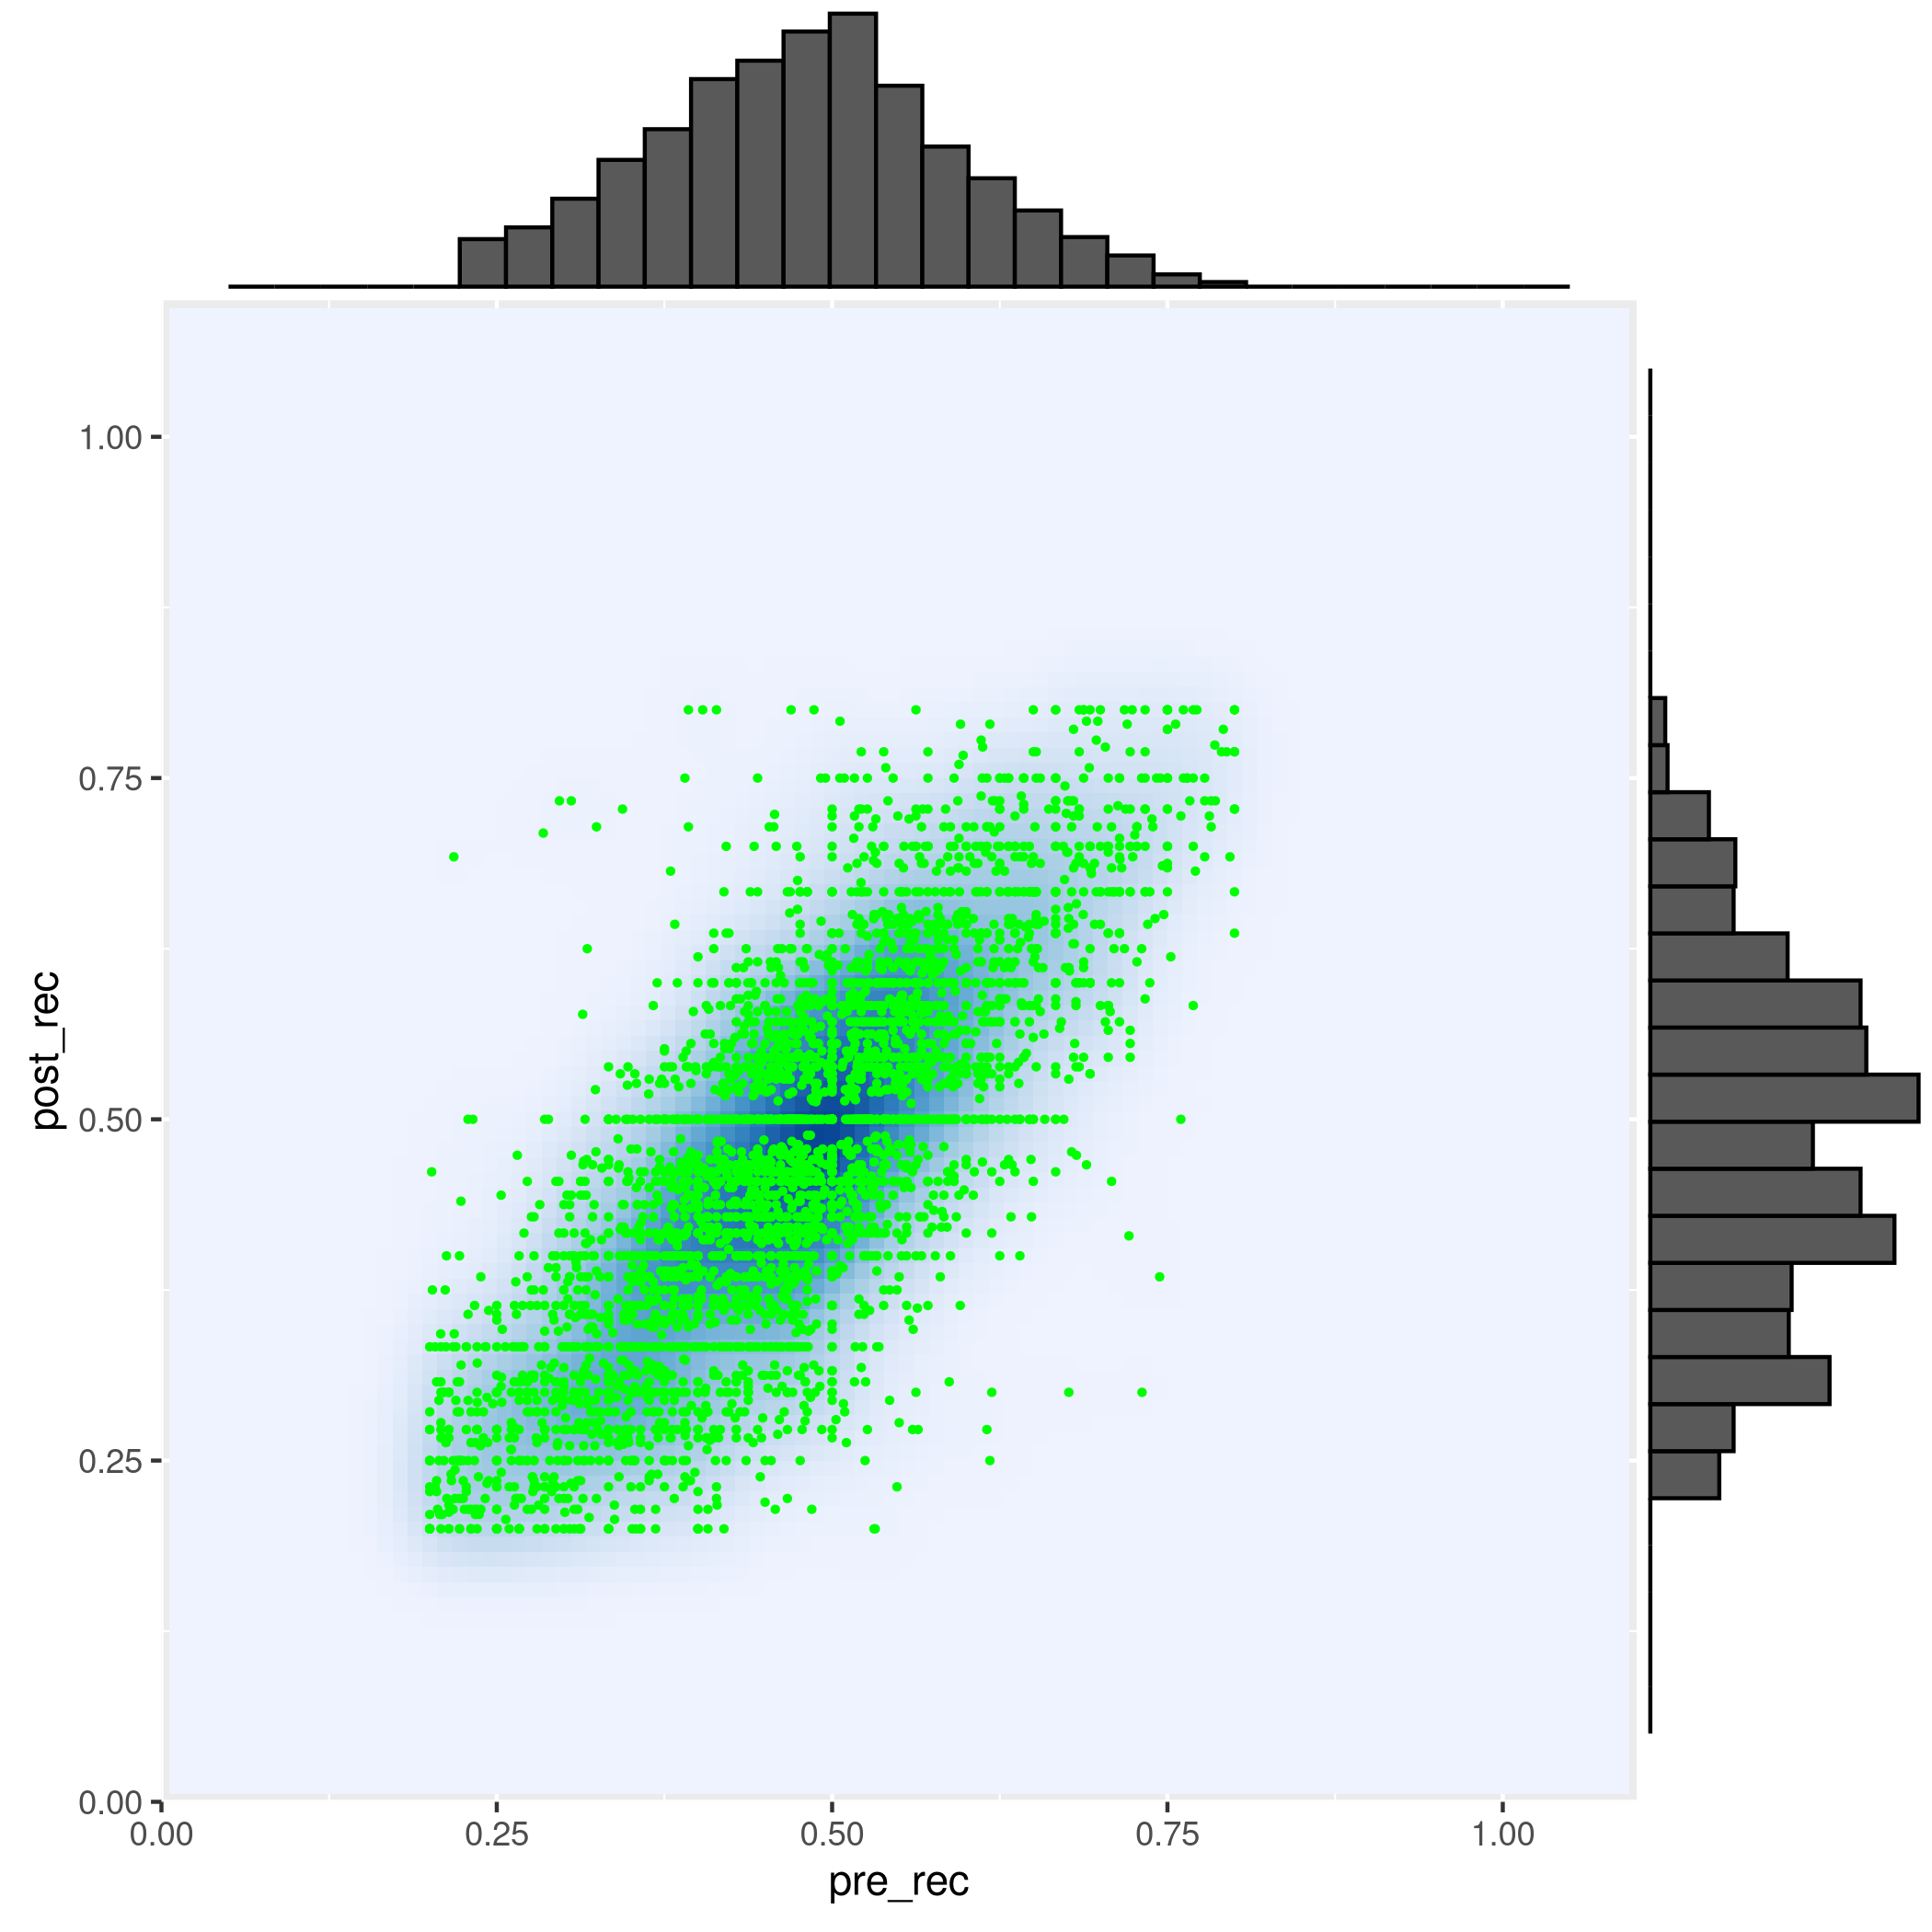
\includegraphics[width = 0.3\textwidth]{correlation_recal/shDHX30_NUTLIN_TOT_1.png}} &
      \subfloat[shPCBP2 DMSO polisomale]{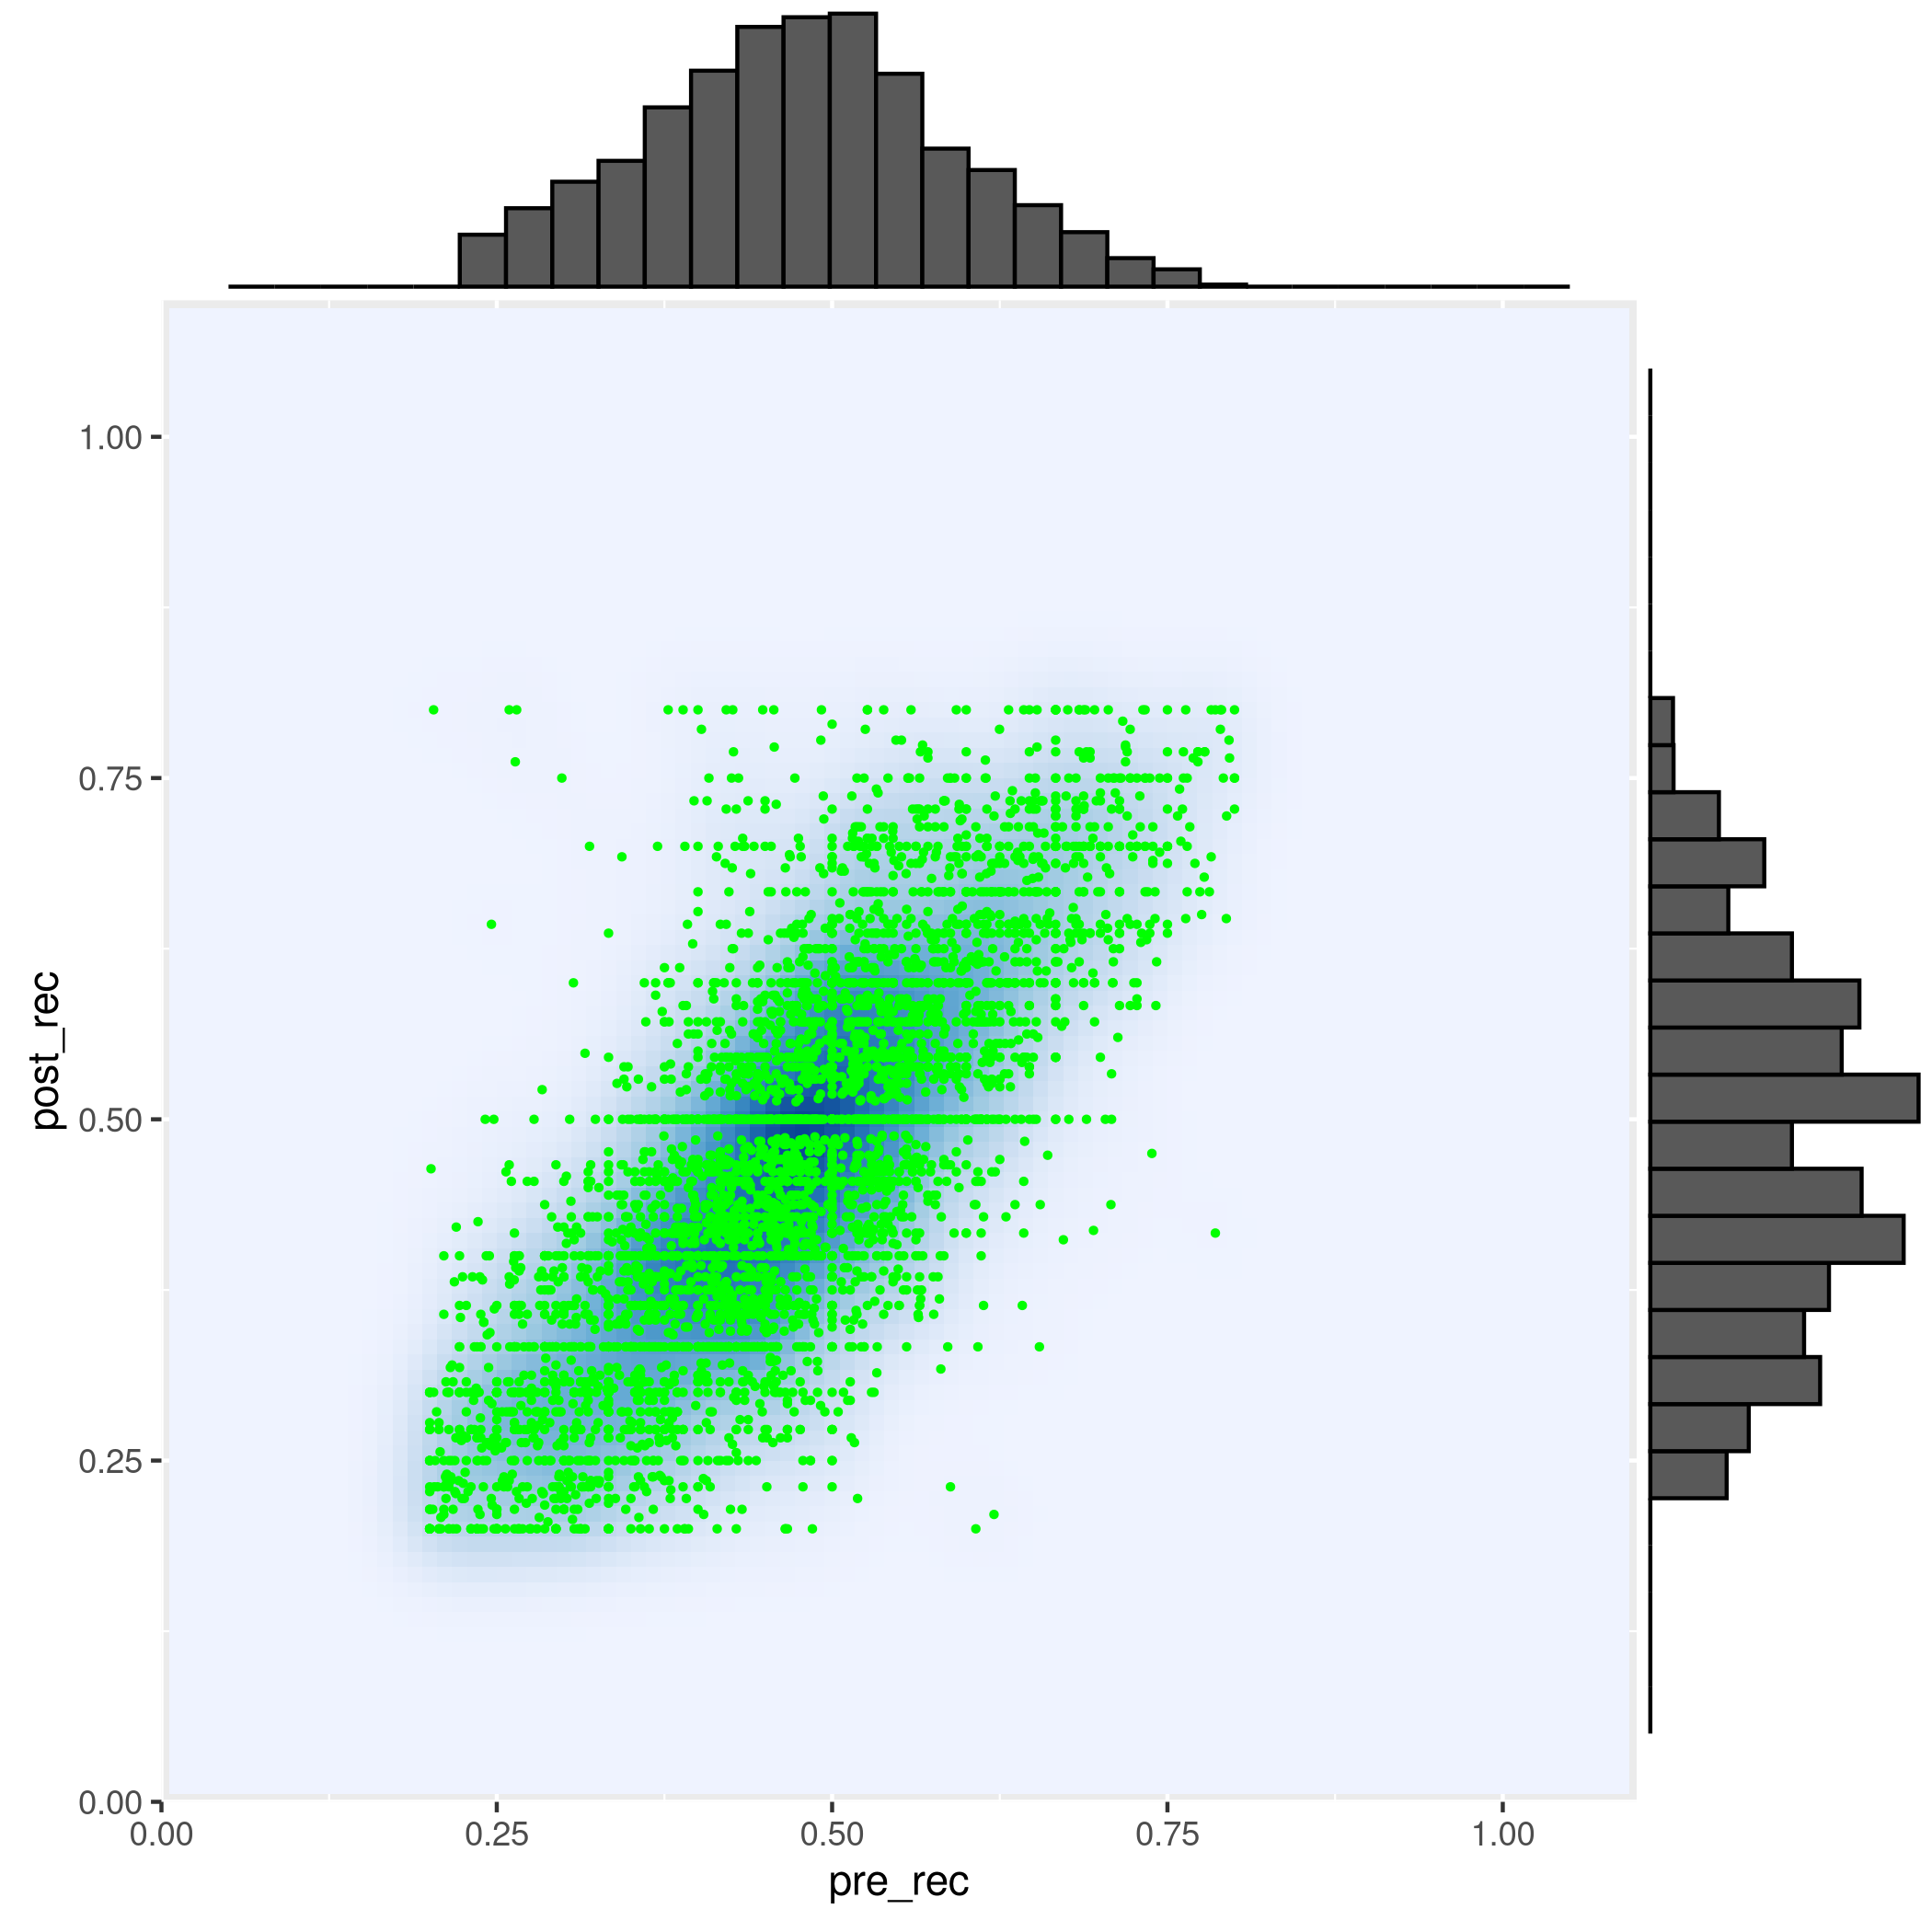
\includegraphics[width = 0.3\textwidth]{correlation_recal/shPCBP2_DMSO_POL_1.png}} \\
      \subfloat[shPCBP2 DMSO totale]{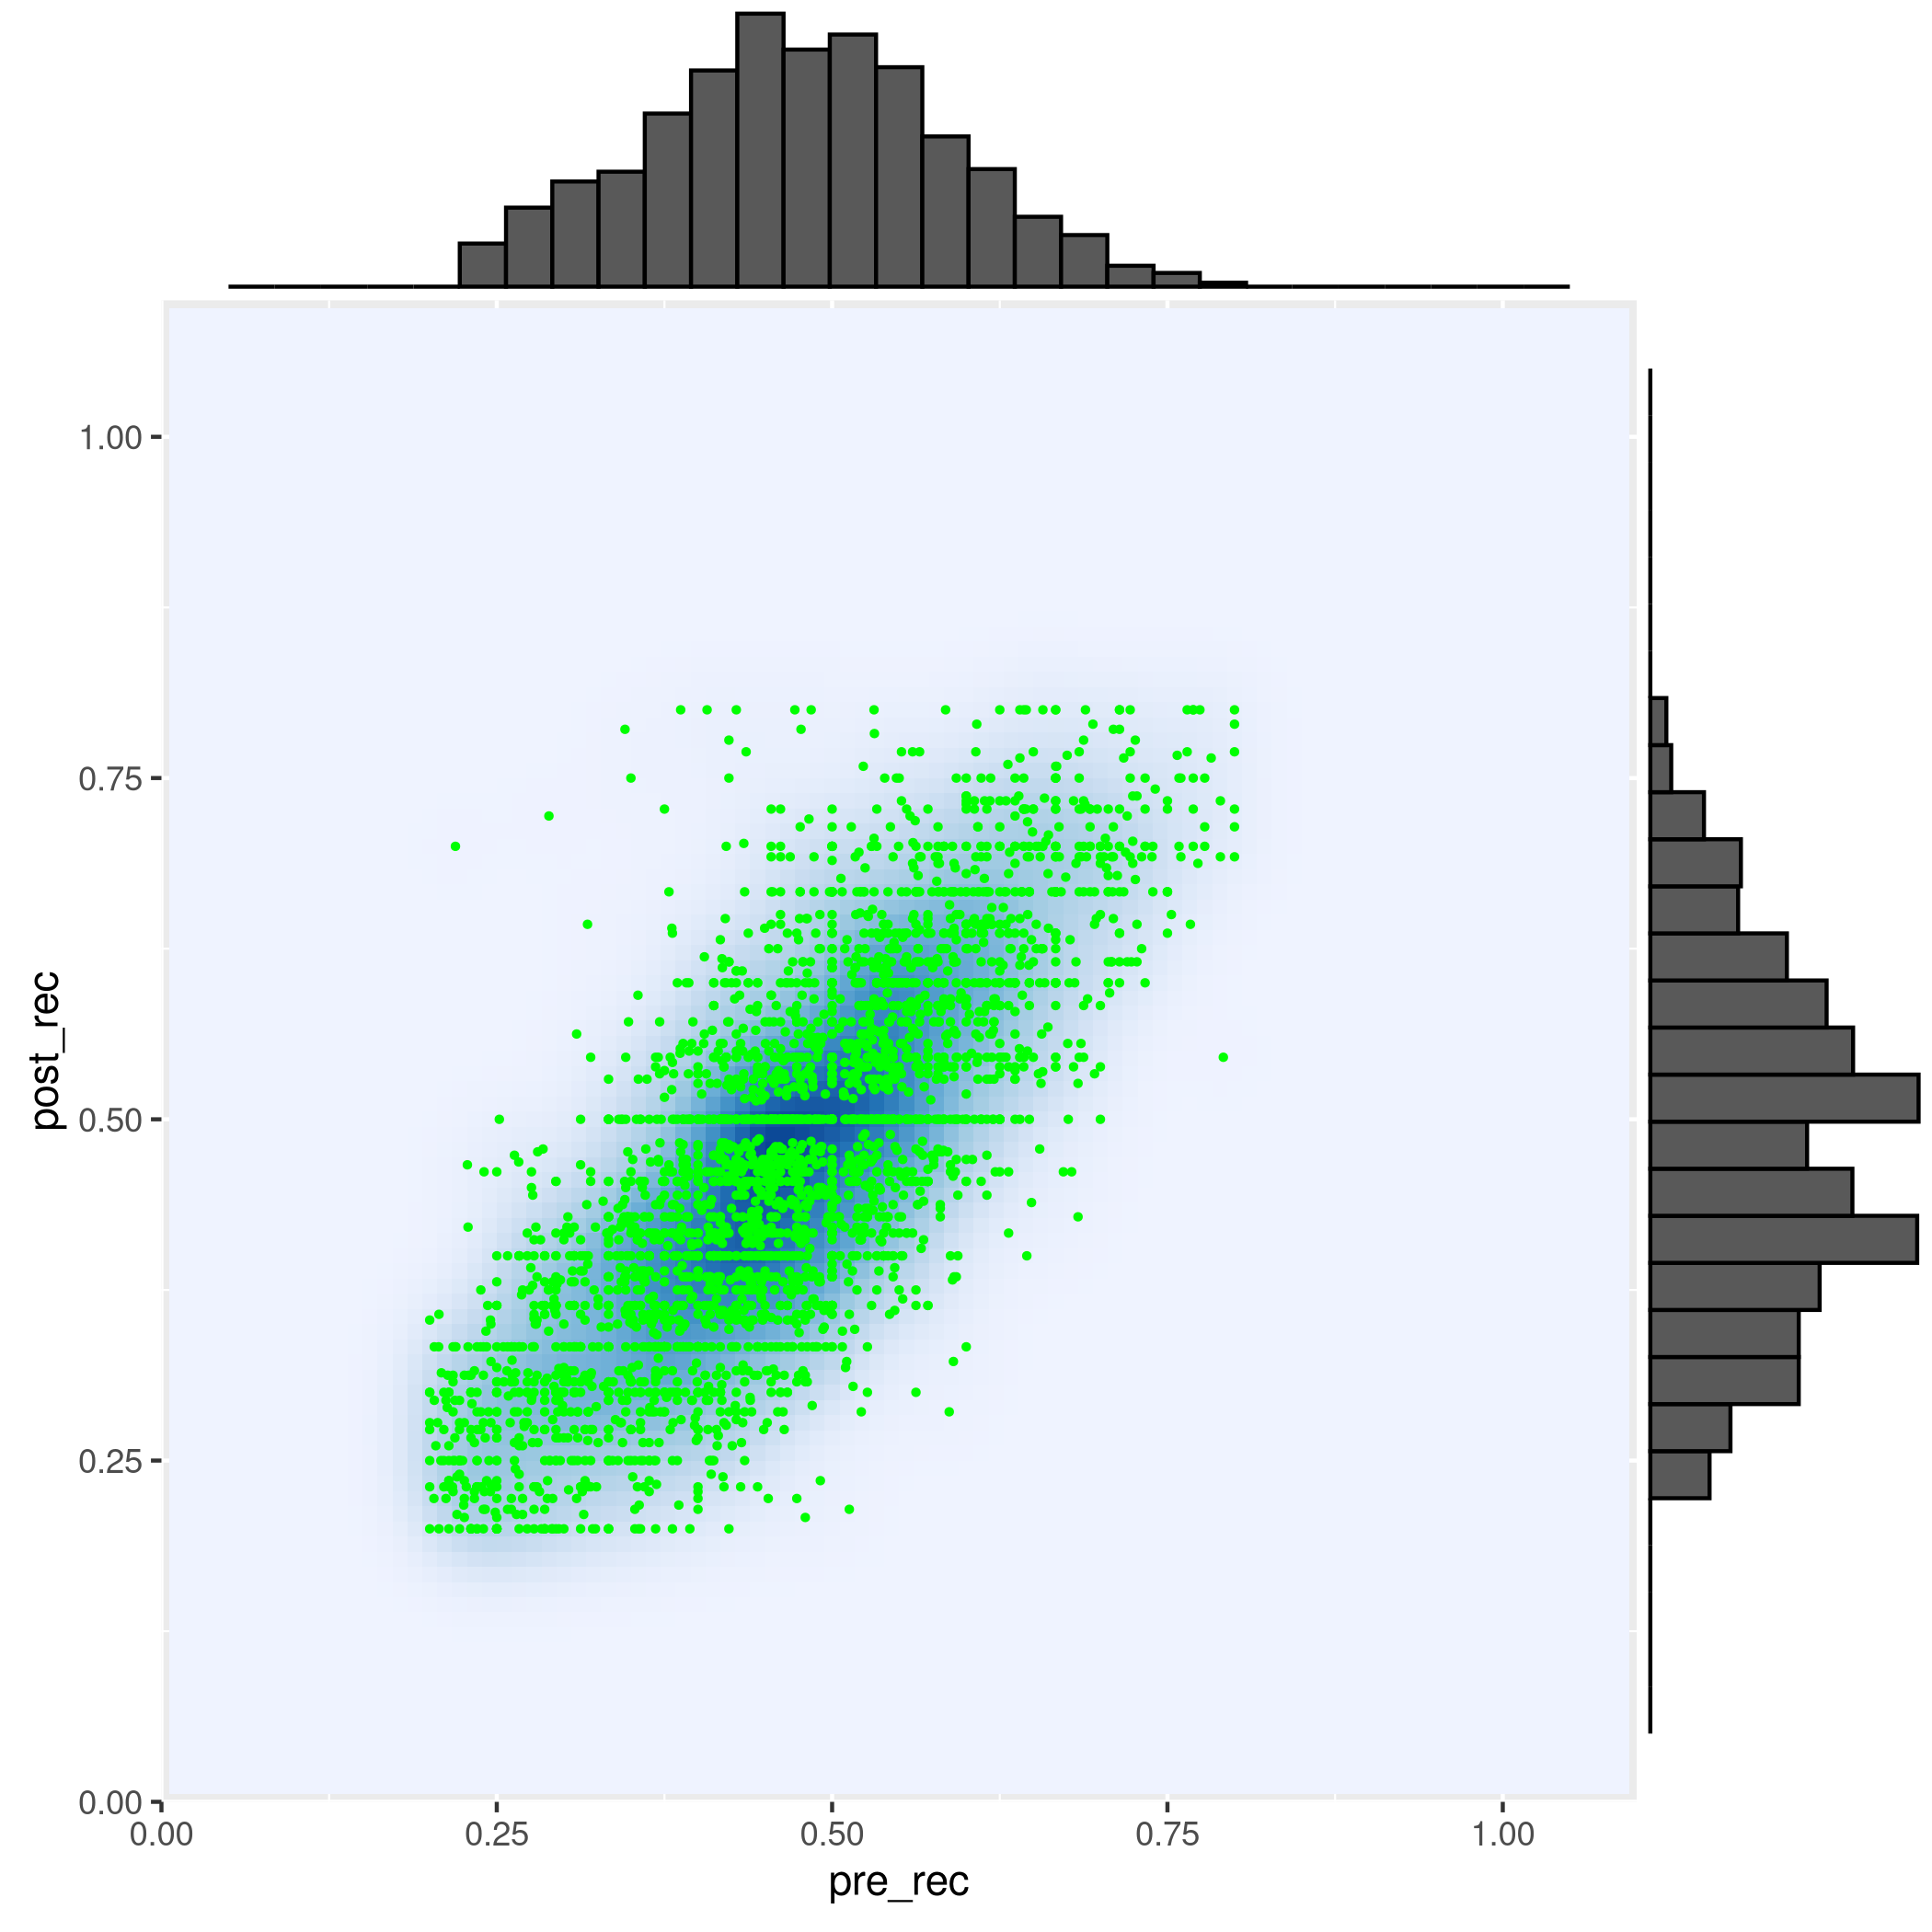
\includegraphics[width = 0.3\textwidth]{correlation_recal/shPCBP2_DMSO_TOT_1.png}} &
      \subfloat[shPCBP2 NUTLIN polisomale]{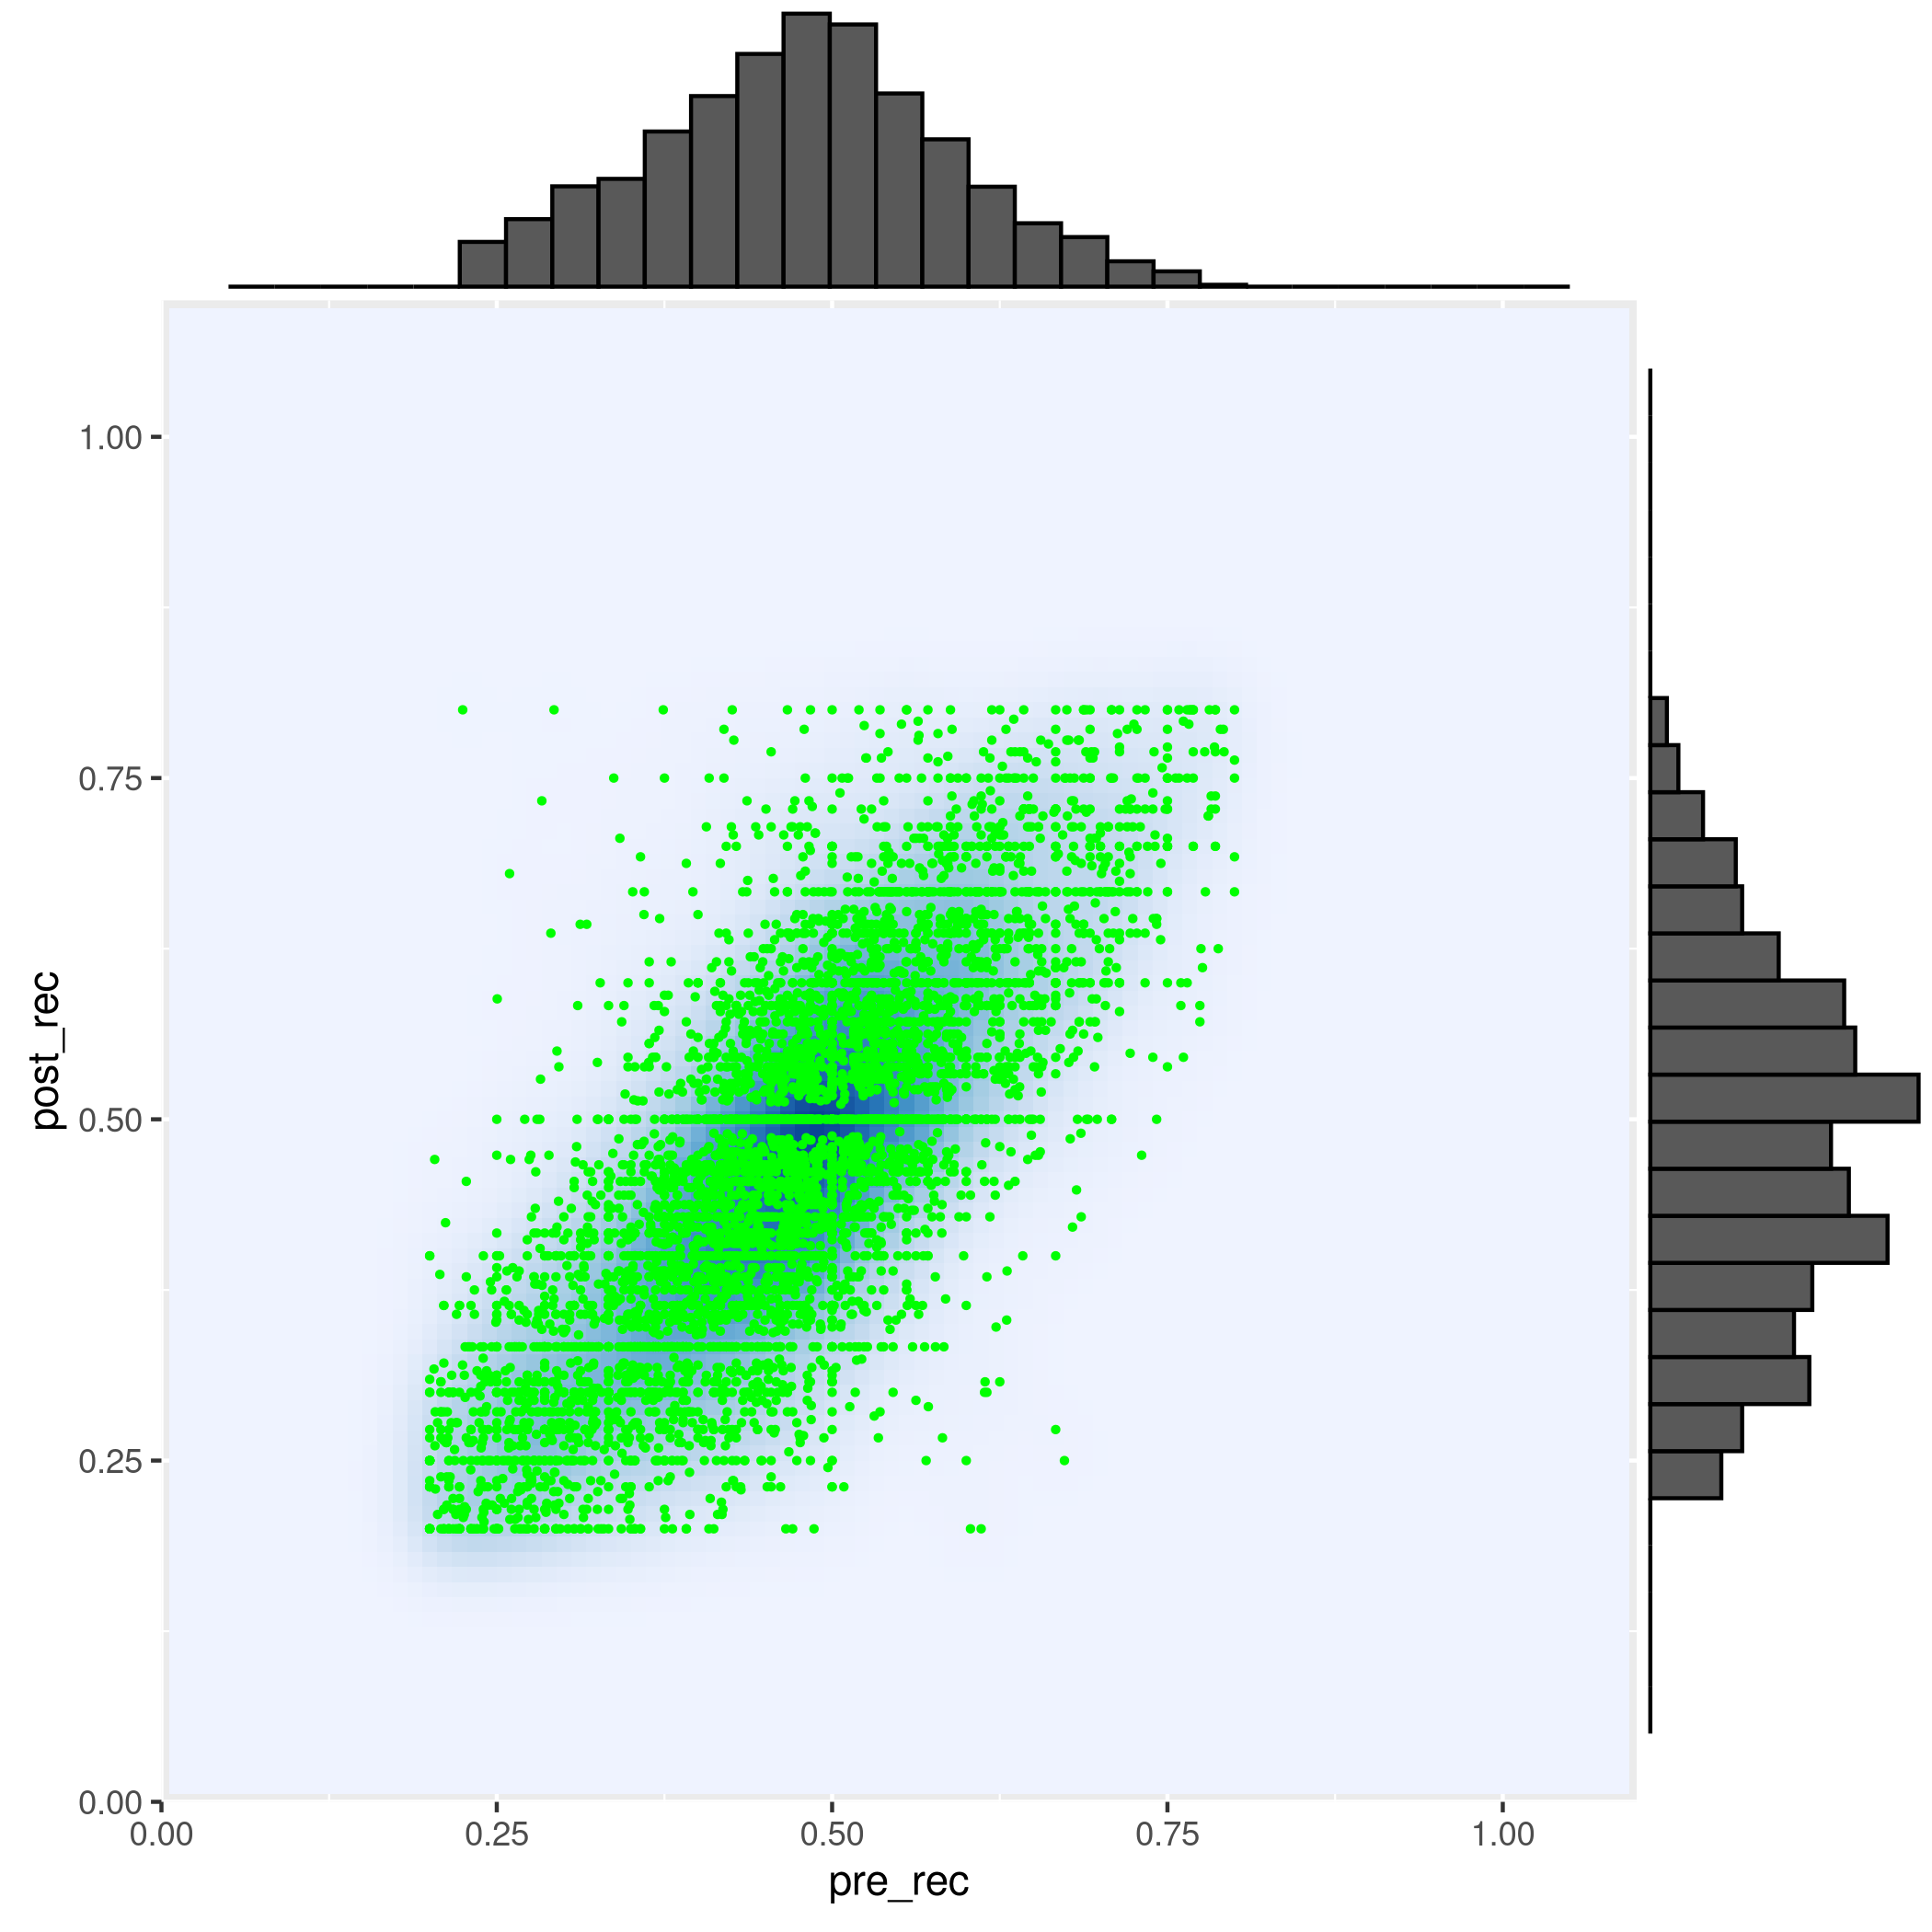
\includegraphics[width = 0.3\textwidth]{correlation_recal/shPCBP2_NUTLIN_POL_1.png}} &
      \subfloat[shPCBP2 NUTLIN totale]{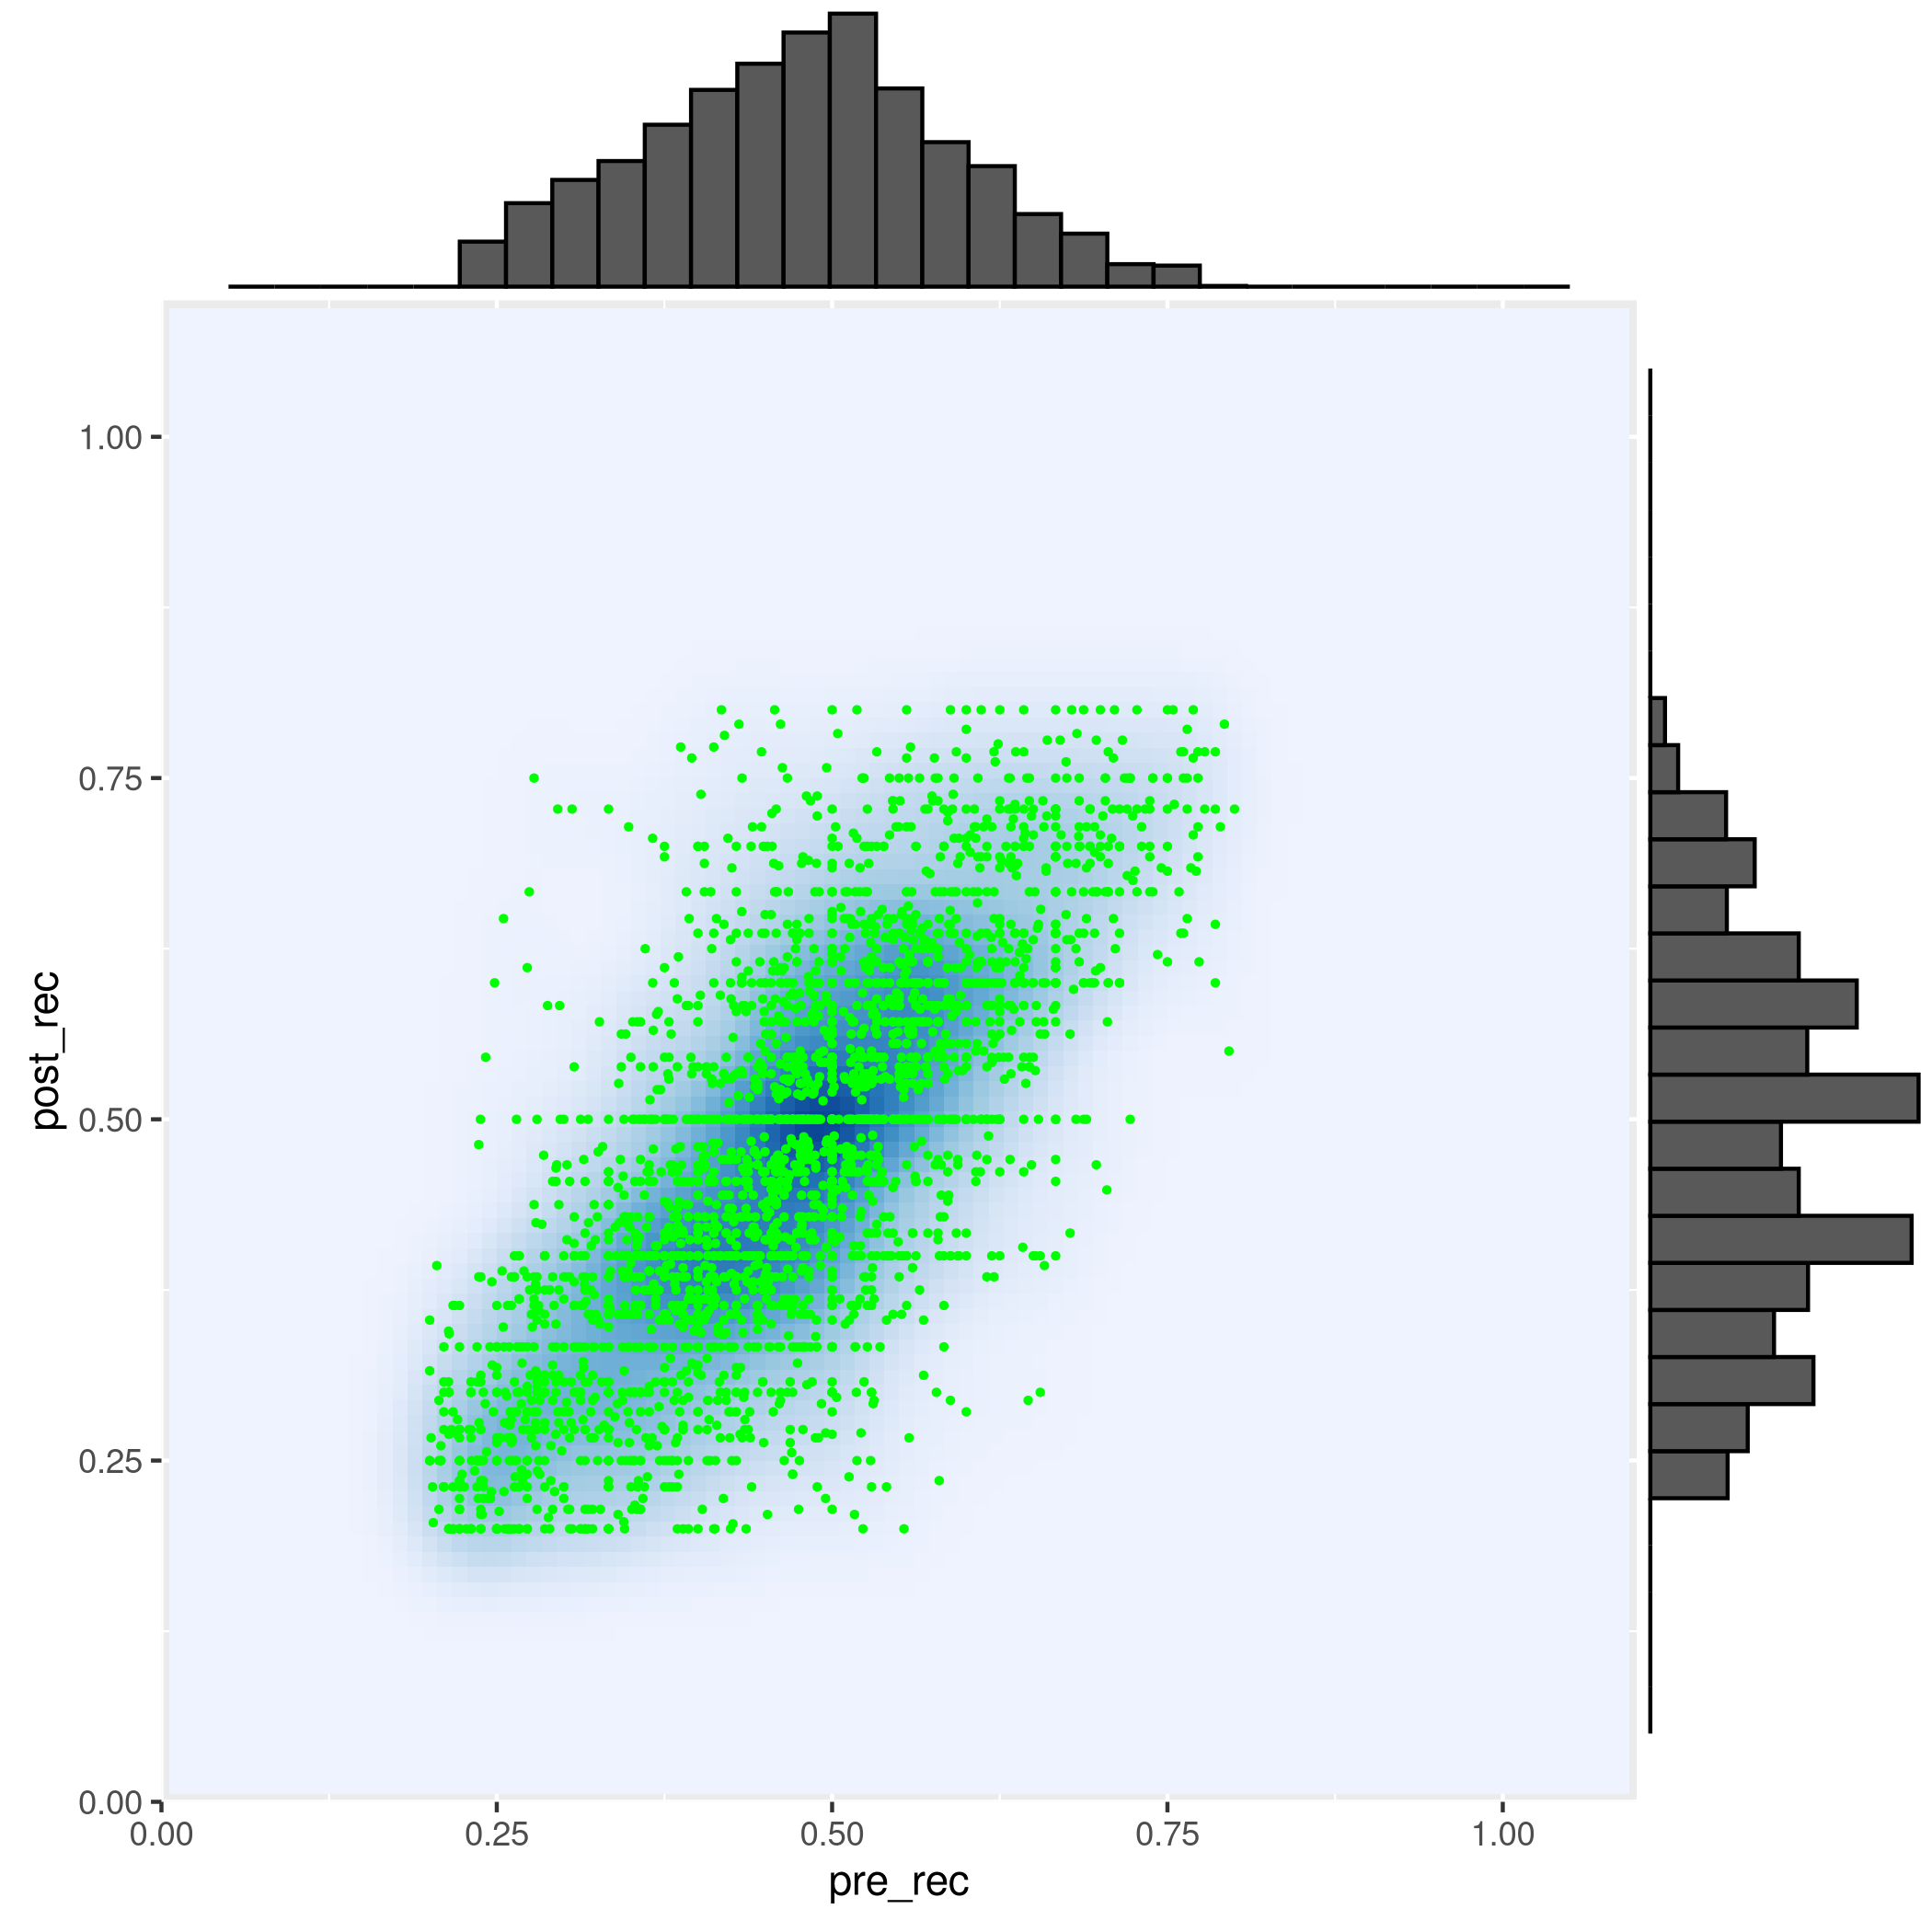
\includegraphics[width = 0.3\textwidth]{correlation_recal/shPCBP2_NUTLIN_TOT_1.png}} \\
  \end{tabular}
   \label{fig:}
 \end{figure}

\section{Ottenere i dati per gli SNP di interesse}
\label{sec:snp_filter}
Discussione degli SNP con i dati necessari per lo studio e scelta degli SNP di interesse.
Ovvero come \`e stata ottenuta la lista da cellminer, i t-test.
Magari qua posso mettere un barplot con la conta degli SNP trovati.

   \subsection{Boxplot}
   I boxplot degli SNP trovati.
 \begin{figure}[H]
   \centering
   \begin{tabular}{cc}
      \subfloat[scr DMSO rs1131941]{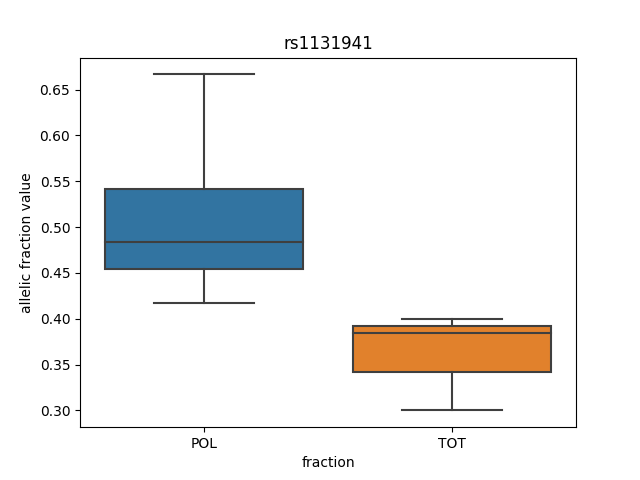
\includegraphics[width = 0.5\textwidth]{boxplot/scr_DMSO_rs1131941.png}} &
      \subfloat[scr DMSO rs2228626]{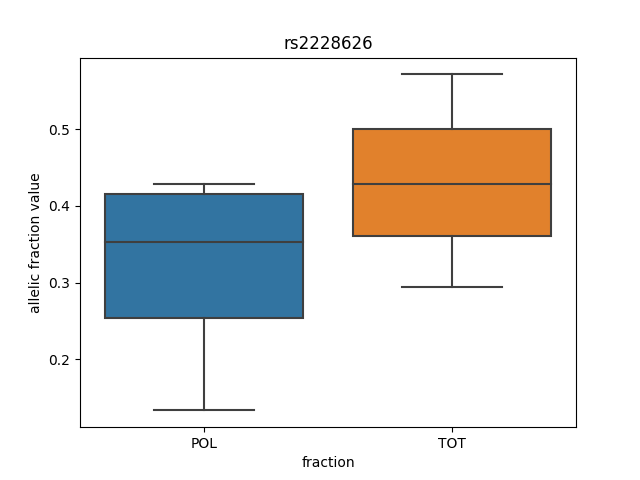
\includegraphics[width = 0.5\textwidth]{boxplot/scr_DMSO_rs2228626.png}} \\
      \subfloat[scr DMSO rs2289373]{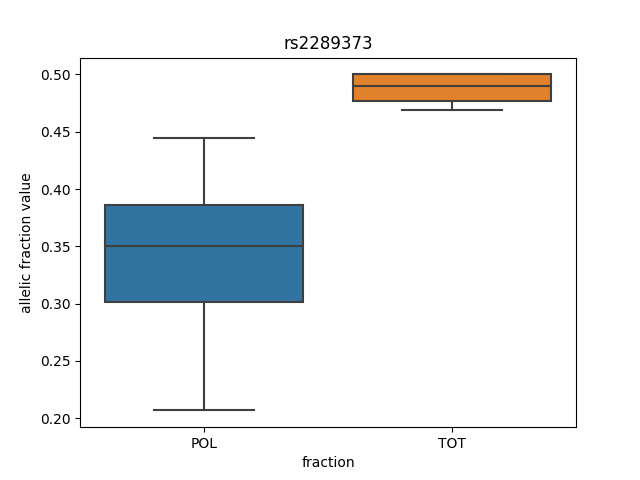
\includegraphics[width = 0.5\textwidth]{boxplot/scr_DMSO_rs2289373.png}} &
      \subfloat[shPCBP2 NUTLIN rs9833]{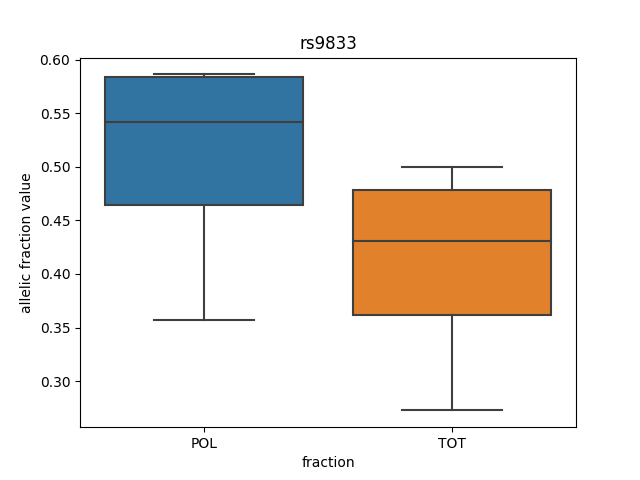
\includegraphics[width = 0.5\textwidth]{boxplot/shPCBP2_NUTLIN_rs9833.png}} \\
  \end{tabular}
   \label{fig:}
 \end{figure}

\section{Caratterizzazione degli SNP di interesse}
Magari una lista contenente gli SNP caratterizzati con snpEff




\section{Conclusioni}
\label{sec:ending}



    \endgroup


    % bibliografia in formato bibtex
    %
    % aggiunta del capitolo nell'indice
    \addcontentsline{toc}{chapter}{Bibliografia}
    % stile con ordinamento alfabetico in funzione degli autori
    \bibliographystyle{acm}
    \bibliography{bibliography/biblio}
%%%%%%%%%%%%%%%%%%%%%%%%%%%%%%%%%%%%%%%%%%%%%%%%%%%%%%%%%%%%%%%%%%%%%%%%%%
%%%%%%%%%%%%%%%%%%%%%%%%%%%%%%%%%%%%%%%%%%%%%%%%%%%%%%%%%%%%%%%%%%%%%%%%%%
%% Nota
%%%%%%%%%%%%%%%%%%%%%%%%%%%%%%%%%%%%%%%%%%%%%%%%%%%%%%%%%%%%%%%%%%%%%%%%%%
%% Nella bibliografia devono essere riportati tutte le fonti consultate
%% per lo svolgimento della tesi. La bibliografia deve essere redatta
%% in ordine alfabetico sul cognome del primo autore.
%%
%% La forma della citazione bibliografica va inserita secondo la fonte utilizzata:
%%
%% LIBRI
%% Cognome e iniziale del nome autore/autori, la data di edizione, titolo, casa editrice, eventuale numero dell’edizione.
%%
%% ARTICOLI DI RIVISTA
%% Cognome e iniziale del nome autore/autori, titolo articolo, titolo rivista, volume, numero, numero di pagine.
%%
%% ARTICOLI DI CONFERENZA
%% Cognome e iniziale del nome autore/autori (anno), titolo articolo, titolo conferenza, luogo della conferenza (città e paese), date della conferenza, numero di pagine.
%%
%% SITOGRAFIA
%% La sitografia contiene un elenco di indirizzi Web consultati e disposti in ordine alfabetico.
%% E’ necessario:
%%   Copiare la URL (l’indirizzo web) specifica della pagina consultata
%%   Se disponibile, indicare il cognome e nome dell’autore, il titolo ed eventuale sottotitolo del testo
%%   Se disponibile, inserire la data di ultima consultazione della risorsa (gg/mm/aaaa).
%%%%%%%%%%%%%%%%%%%%%%%%%%%%%%%%%%%%%%%%%%%%%%%%%%%%%%%%%%%%%%%%%%%%%%%%%%
%%%%%%%%%%%%%%%%%%%%%%%%%%%%%%%%%%%%%%%%%%%%%%%%%%%%%%%%%%%%%%%%%%%%%%%%%%


    \titleformat{\chapter}
        {\normalfont\Huge\bfseries}{Allegato \thechapter}{1em}{}
    % sezione Allegati - opzionale
    \appendix
    %\chapter{Titolo primo allegato}

\section{Titolo}

\subsection{Sottotitolo}

\chapter{Titolo secondo allegato}

\section{Titolo}

\subsection{Sottotitolo}


\end{document}
